\documentclass[twocolumn,10pt,a4paper]{article}

% Page layout
\usepackage[margin=2cm, columnsep=0.6cm]{geometry}

% Packages
\usepackage[utf8]{inputenc}
\usepackage[T1]{fontenc}
\usepackage{amsmath,amssymb,amsfonts,amsthm}
\usepackage{mathtools}
\usepackage{physics}
\usepackage{geometry}
\usepackage{graphicx}
\usepackage{float}
\usepackage{booktabs}
\usepackage{array}
\usepackage{hyperref}
\usepackage{natbib}
\usepackage{siunitx}
\usepackage{import}
\usepackage{enumitem}



% Theorem environments
\newtheorem{theorem}{Theorem}[section]
\newtheorem{lemma}[theorem]{Lemma}
\newtheorem{corollary}[theorem]{Corollary}
\newtheorem{proposition}[theorem]{Proposition}
\newtheorem{definition}[theorem]{Definition}
\newtheorem{axiom}{Axiom}
\theoremstyle{remark}
\newtheorem{remark}[theorem]{Remark}
\newtheorem{example}[theorem]{Example}

% Custom commands
\newcommand{\hilbert}{\mathcal{H}}
\newcommand{\manifold}{\mathcal{M}}
\newcommand{\partition}{\mathcal{P}}
\newcommand{\oscillator}{\mathcal{O}}
\newcommand{\instrument}{\mathcal{I}}
\newcommand{\kB}{k_{\mathrm{B}}}
\newcommand{\Reals}{\mathbb{R}}
\newcommand{\Integers}{\mathbb{Z}}
\newcommand{\Naturals}{\mathbb{N}}
\newcommand{\Complex}{\mathbb{C}}

\title{\textbf{On the Necessity of Frequency-Selective Coupling Structures\\in Bounded Oscillatory Systems}}

\author{
Kundai Farai Sachikonye\\
\texttt{kundai.sachikonye@wzw.tum.de}
}

\date{\today}

\begin{document}

\maketitle

\begin{abstract}

We establish that frequency-selective coupling structures arise as mathematical necessities in bounded measure-preserving dynamical systems admitting categorical observation. From two axioms—bounded phase space volume $\mu(M) < \infty$ and finite observer resolution—we derive a four-parameter coordinate system $(n, \ell, m, s)$ characterising the complete space of distinguishable states under nested partition geometry. We prove that information extraction from such systems requires oscillatory coupling between observer and observed, with frequency matching conditions $|\omega_{\text{obs}} - \omega_{\text{sys}}| < \Delta\omega$ partitioning the space of admissible couplings into discrete selective channels.

Our central result, the \textbf{Instrument Necessity Theorem}, establishes that for each partition coordinate $\xi \in \{n, \ell, m, s\}$, there exists a unique minimal coupling structure $\mathcal{I}_\xi$ satisfying:
\begin{enumerate}[label=(\roman*)]
    \item $\mathcal{I}_\xi$ extracts coordinate $\xi$ with efficiency $\eta_\xi \geq \eta_{\min}$,
    \item $\mathcal{I}_\xi$ remains invariant under transformations of complementary coordinates $\{\zeta \in \{n,\ell,m,s\} : \zeta \neq \xi\}$,
    \item $\mathcal{I}_\xi$ is minimal in the sense that any proper sub-structure fails condition (i) or (ii).
\end{enumerate}
We derive explicit frequency-coordinate dualities through dimensional analysis of the partition geometry, mapping each coordinate to characteristic frequency regimes via
\begin{equation}
\omega_\xi = \frac{E_\xi}{\hbar} = \frac{k_B T}{\hbar} f_\xi(n, \ell, m, s),
\end{equation}
where $f_\xi$ are dimensionless functions determined by the partition topology. We prove that the collection $\{\mathcal{I}_n, \mathcal{I}_\ell, \mathcal{I}_m, \mathcal{I}_s\}$ forms a complete measurement basis: the algebra generated by compositions $\mathcal{I}_{\xi_1} \circ \mathcal{I}_{\xi_2} \circ \cdots \circ \mathcal{I}_{\xi_k}$ is dense in the space of all bounded linear operators on the observable algebra.

We establish fundamental bounds on coupling efficiency through the uncertainty relation
\begin{equation}
\eta_\xi \leq \frac{\Delta\omega \cdot \Delta t}{\hbar/E_\xi} \leq 1,
\end{equation}
We prove that measurement precision is constrained by the time-frequency product. The framework yields quantitative predictions for transition frequencies $\omega_{n\ell ms \to n'\ell'm's'}$, selection rules (vanishing matrix elements), and coupling strengths $g_{\xi\xi'}$, all expressed in terms of fundamental constants $(\hbar, k_B, c, \mu_0, \epsilon_0)$ with zero free parameters.

The derived coupling structures correspond bijectively to known spectroscopic instrumentation:
\begin{align}
\mathcal{I}_n &\longleftrightarrow \text{Absorption/emission spectroscopy (electronic transitions)}, \\
\mathcal{I}_\ell &\longleftrightarrow \text{Raman spectroscopy (vibrational modes)}, \\
\mathcal{I}_m &\longleftrightarrow \text{Magnetic resonance (orientational states)}, \\
\mathcal{I}_s &\longleftrightarrow \text{Circular dichroism (chiral discrimination)}.
\end{align}
This correspondence is not phenomenological but follows from the isomorphism between the abstract coupling structures $\{\mathcal{I}_\xi\}$ and the electromagnetic interaction Hamiltonians $\{H_{\text{int}}^\xi\}$ governing photon-matter coupling. We conclude that spectroscopic instruments instantiate geometric necessities: the structure of measurement apparatus is uniquely determined by the mathematics of bounded categorical observation, with the four fundamental spectroscopic modalities exhausting the complete set of elementary measurements on partition coordinates.

\textbf{Measure-preserving dynamical systems \and Categorical observation \and Frequency-selective coupling \and Spectroscopic instrumentation \and Partition coordinates \and Oscillatory resonance \and Information extraction \and Bounded phase space \and Instrument necessity theorem \and Measurement completeness}

\end{abstract}


\section{Introduction}
\label{sec:introduction}

The extraction of information from physical systems through measurement constitutes a foundational operation in experimental science, yet the mathematical principles governing the structure of measurement apparatus remain incompletely understood. While spectroscopic instrumentation has been developed through iterative empirical refinement and domain-specific engineering optimization, a fundamental question persists: \emph{to what extent does the architecture of measurement devices necessarily follow from the mathematical properties of the systems under observation?} 

We address this question through a first-principles analysis of information extraction from bounded measure-preserving dynamical systems. Our central thesis is that the structure of frequency-selective coupling mechanisms—and by extension, the architecture of spectroscopic instrumentation—arises not from contingent engineering choices but from geometric necessities inherent in the mathematics of categorical observation in bounded phase spaces.

\subsection{Motivation and Scope}

Consider the following empirical observation: spectroscopic techniques across diverse physical domains exhibit remarkable structural similarities despite arising from independent historical developments. Absorption spectroscopy, Raman spectroscopy, magnetic resonance, and circular dichroism—while probing ostensibly different physical phenomena—share common features: frequency-selective coupling, resonance conditions, selection rules, and characteristic transition frequencies. This convergence suggests an underlying mathematical structure constraining the space of possible measurement operations.

We demonstrate that this structure necessarily follows from two axioms:
\begin{enumerate}[label=(\roman*)]
    \item \textbf{Bounded phase space}: The system under observation occupies a manifold $\manifold$ of finite measure $\mu(\manifold) < \infty$.
    \item \textbf{Finite observer resolution}: Any physical observer can distinguish only finitely many states, requiring a partition $\partition$ of $\manifold$ into $N < \infty$ operationally distinguishable categories.
\end{enumerate}

From these axioms alone, we derive: (a) the necessity of oscillatory coupling for information extraction, (b) the emergence of a four-parameter coordinate system $(n,\ell,m,s)$ characterising distinguishable states, (c) explicit frequency-coordinate dualities mapping coordinates to characteristic frequency regimes, and (d) the existence of minimal coupling structures $\{\mathcal{I}_n, \mathcal{I}_\ell, \mathcal{I}_m, \mathcal{I}_s\}$ forming a complete measurement basis.

\subsection{Mathematical Framework}

Our analysis proceeds within the framework of ergodic theory and measure-preserving dynamical systems \citep{Poincare1890, Birkhoff1931, Kolmogorov1954}. Let $(\manifold, \mu, \phi_t)$ denote a measure-preserving dynamical system where:
\begin{itemize}
    \item $\manifold$ is a smooth compact manifold (the phase space),
    \item $\mu$ is a finite Borel measure with $\mu(\manifold) < \infty$ (the invariant measure),
    \item $\phi_t: \manifold \to \manifold$ is a one-parameter group of measure-preserving diffeomorphisms satisfying $\mu(\phi_t(A)) = \mu(A)$ for all measurable $A \subseteq \manifold$ and $t \in \mathbb{R}$.
\end{itemize}

The Poincaré recurrence theorem \citep{Poincare1890} guarantees that for almost every initial condition $x_0 \in \manifold$, the trajectory $\phi_t(x_0)$ returns arbitrarily close to $x_0$ infinitely often:
\begin{equation}
\forall \epsilon > 0, \; \exists \, t_n \to \infty \text{ such that } d(\phi_{t_n}(x_0), x_0) < \epsilon.
\end{equation}
This recurrence property implies that bounded measure-preserving systems generically exhibit oscillatory or quasi-periodic dynamics, establishing oscillatory behavior as a mathematical necessity rather than a special case.

We model an \emph{observer} as a measurable partition $\partition = \{P_1, P_2, \ldots, P_N\}$ of $\manifold$ satisfying:
\begin{equation}
\bigcup_{i=1}^N P_i = \manifold, \quad P_i \cap P_j = \emptyset \; (i \neq j), \quad \mu(P_i) > 0 \; \forall i.
\end{equation}
States $x, y \in P_i$ are operationally indistinguishable to the observer, defining an equivalence relation on $\manifold$. The partition $\partition$ induces a discrete observable algebra $\mathcal{A}_\partition$ consisting of functions constant on partition elements, with dimension $\dim(\mathcal{A}_\partition) = N$.

The \emph{information extraction problem} is formulated as follows: given a system in unknown state $x \in \manifold$, construct a coupling mechanism that determines the partition element $P_i$ containing $x$ through interaction with an auxiliary system (the measurement apparatus). We seek to characterize:
\begin{enumerate}[label=(\alph*)]
    \item The minimal structure required of coupling mechanisms to extract partition information,
    \item The constraints governing the form of such coupling mechanisms,
    \item The completeness properties of the space of coupling mechanisms,
    \item The relationship between abstract coupling structures and physical measurement devices.
\end{enumerate}

\subsection{Coupling Structures and Information Extraction}

A \emph{coupling structure} is defined as a triple $(\oscillator, \nu, \psi_t, \Gamma)$ where:
\begin{itemize}
    \item $(\oscillator, \nu, \psi_t)$ is an auxiliary measure-preserving dynamical system (the observer/apparatus),
    \item $\Gamma: \manifold \times \oscillator \to \mathbb{R}$ is a coupling function specifying the interaction energy between system and apparatus.
\end{itemize}

The coupled dynamics evolve under the Hamiltonian
\begin{equation}
H_{\text{total}}(x, y) = H_{\text{sys}}(x) + H_{\text{obs}}(y) + \lambda \Gamma(x, y),
\end{equation}
where $\lambda$ is the coupling strength. Information extraction occurs when the apparatus state $y(t)$ becomes correlated with the system partition coordinate through the coupling $\Gamma$.

Our central question is: \emph{what properties must $\Gamma$ possess to enable extraction of partition coordinate information?} We prove that frequency-selective coupling is not merely sufficient but \emph{necessary}: any coupling structure capable of extracting partition information must exhibit frequency selectivity, with resonance conditions determining which coordinates are accessible.

\subsection{Principal Results}

Our main contributions are:

\begin{enumerate}
    \item \textbf{Partition Coordinate Theorem} (Section~\ref{sec:partition_coordinates}): We prove that any partition of a bounded measure-preserving system respecting natural geometric constraints admits a canonical four-parameter coordinate system $(n,\ell,m,s)$ where:
    \begin{itemize}
        \item $n \in \mathbb{N}$ indexes nested hierarchical levels (depth coordinate),
        \item $\ell \in \{0, 1, \ldots, n-1\}$ indexes complexity within level $n$ (angular momentum analogue),
        \item $m \in \{-\ell, -\ell+1, \ldots, \ell\}$ indexes orientation (magnetic quantum number analogue),
        \item $s \in \{-1/2, +1/2\}$ indexes chirality (spin analogue).
    \end{itemize}
    
    \item \textbf{Frequency-Coordinate Duality} (Section~\ref{sec:frequency_coordinate_duality}): We derive explicit mappings between partition coordinates and characteristic frequency regimes through dimensional analysis:
    \begin{equation}
    \omega_\xi = \frac{k_B T}{\hbar} f_\xi(n, \ell, m, s),
    \end{equation}
    where $f_\xi$ are dimensionless functions determined by partition topology. These dualities establish that coordinate transitions $\xi \to \xi'$ correspond to frequency absorption/emission at $\omega_{\xi\xi'} = |\omega_\xi - \omega_{\xi'}|$.
    
    \item \textbf{Instrument Necessity Theorem} (Section~\ref{sec:instrument_necessity}): For each coordinate $\xi \in \{n,\ell,m,s\}$, we prove the existence and uniqueness of a minimal coupling structure $\mathcal{I}_\xi$ satisfying:
    \begin{enumerate}[label=(\roman*)]
        \item \emph{Extraction}: $\mathcal{I}_\xi$ extracts coordinate $\xi$ with efficiency $\eta_\xi \geq \eta_{\min}$,
        \item \emph{Invariance}: $\mathcal{I}_\xi$ remains invariant under transformations of complementary coordinates,
        \item \emph{Minimality}: Any proper sub-structure of $\mathcal{I}_\xi$ fails condition (i) or (ii).
    \end{enumerate}
    The coupling functions $\Gamma_\xi$ are uniquely determined (up to isomorphism) by these conditions.
    
    \item \textbf{Completeness Theorem} (Section~\ref{sec:completeness}): We prove that the collection $\{\mathcal{I}_n, \mathcal{I}_\ell, \mathcal{I}_m, \mathcal{I}_s\}$ forms a complete measurement basis: the operator algebra generated by compositions
    \begin{equation}
    \mathcal{I}_{\xi_1} \circ \mathcal{I}_{\xi_2} \circ \cdots \circ \mathcal{I}_{\xi_k}
    \end{equation}
    is dense in the space of all bounded linear operators on $\mathcal{A}_\partition$. This establishes that any measurement on partition coordinates decomposes into these four elementary operations.
    
    \item \textbf{Spectroscopic Correspondence} (Section~\ref{sec:discussion}): We establish a bijection between abstract coupling structures and known spectroscopic techniques:
    \begin{align}
    \mathcal{I}_n &\longleftrightarrow \text{Absorption/emission spectroscopy}, \\
    \mathcal{I}_\ell &\longleftrightarrow \text{Raman spectroscopy}, \\
    \mathcal{I}_m &\longleftrightarrow \text{Magnetic resonance spectroscopy}, \\
    \mathcal{I}_s &\longleftrightarrow \text{Circular dichroism spectroscopy}.
    \end{align}
    This correspondence follows from the isomorphism between abstract coupling functions $\Gamma_\xi$ and electromagnetic interaction Hamiltonians $H_{\text{int}}^\xi$ governing photon-matter coupling.
\end{enumerate}

\subsection{Methodological Approach}

Our derivation proceeds through pure mathematical analysis, independent of specific physical realisations. We do not assume quantum mechanics, electromagnetic theory, or any particular dynamical equations. Instead, we work within the abstract framework of measure-preserving dynamical systems and categorical observation, deriving coupling structures from geometric constraints alone.

This approach yields several advantages:
\begin{itemize}
    \item \textbf{Generality}: The results apply to any bounded measure-preserving system, regardless of physical domain.
    \item \textbf{Necessity}: The derived structures are mathematically necessary, not contingent on physical assumptions.
    \item \textbf{Predictivity}: The framework makes quantitative predictions with zero free parameters.
    \item \textbf{Unification}: Disparate spectroscopic techniques emerge as manifestations of a single mathematical structure.
\end{itemize}

\subsection{Relationship to Prior Work}

Our work intersects several established research areas while introducing novel perspectives:

\textbf{Ergodic theory and dynamical systems.} The foundational results of Poincaré \citep{Poincare1890}, Birkhoff \citep{Birkhoff1931}, and Kolmogorov \citep{Kolmogorov1954} establish the recurrence and mixing properties of measure-preserving systems. We extend this framework by introducing categorical observation and deriving the necessity of frequency-selective coupling for information extraction.

\textbf{Measurement theory and quantum mechanics.} Von Neumann's measurement theory \citep{vonNeumann1932} and subsequent developments \citep{Zurek2003, Schlosshauer2007} address measurement in quantum systems. Our approach is complementary: we work at the level of classical measure-preserving dynamics, deriving measurement structures from geometric constraints rather than quantum postulates. The emergence of quantum-like selection rules and discrete spectra from purely classical considerations is noteworthy.

\textbf{Information theory and statistical mechanics.} Shannon's information theory \citep{Shannon1948} and Jaynes' maximum entropy principle \citep{Jaynes1957} provide frameworks for quantifying information content. We extend these ideas to the dynamical setting, proving that information extraction requires frequency-selective coupling, with efficiency bounds determined by time-frequency uncertainty relations.

\textbf{Spectroscopy and molecular physics.} The empirical development of spectroscopic techniques spans centuries \citep{Herzberg1950, Atkins2011}. Our contribution is to demonstrate that the structure of these techniques necessarily follows from mathematical principles, providing a unified foundation for understanding why spectroscopy takes the forms it does.

\subsection{Organization}

The paper is organised as follows. Part~I (Sections~\ref{sec:bounded_systems}--\ref{sec:frequency_coordinate_duality}) develops the mathematical foundations: bounded oscillatory systems, partition coordinates, and frequency-coordinate duality. Part~II (Sections~\ref{sec:instrument_necessity}--\ref{sec:explicit_coupling}) presents the coupling theory: instrument necessity, resonance conditions, and explicit coupling structures. Part~III (Sections~\ref{sec:completeness}--\ref{sec:minimal_hardware}) establishes completeness results and derives minimal hardware bounds. Section~\ref{sec:discussion} discusses implications, and Section~\ref{sec:conclusion} concludes with structural correspondences to physical spectroscopy.

Throughout, we maintain mathematical rigour while emphasising physical interpretability. Proofs are provided in full, with technical details relegated to the appendices where appropriate. The framework is developed axiomatically, with each result following deductively from the stated assumptions.

\subsection{Notation and Conventions}

Throughout, we employ the following notation:
\begin{itemize}[noitemsep]
    \item $\manifold$: phase space manifold with $\mu(\manifold) < \infty$
    \item $\partition$: categorical partition of $\manifold$
    \item $(n, l, m, s)$: partition coordinates with $n \in \Integers^+$, $l \in \{0, \ldots, n-1\}$, $m \in \{-l, \ldots, l\}$, $s \in \{-\tfrac{1}{2}, +\tfrac{1}{2}\}$
    \item $\omega_\xi$: characteristic frequency associated with coordinate $\xi$
    \item $\instrument_\xi$: minimal coupling structure for coordinate $\xi$
    \item $\langle \cdot, \cdot \rangle$: inner product on the appropriate function space
    \item $[\cdot, \cdot]$: commutator or Poisson bracket as context determines
\end{itemize}

We work in units where dimensional quantities are expressed in terms of a fundamental frequency scale $\omega_0$ and length scale $\ell_0$, with explicit unit restoration in final expressions.


%============================================================
% PART I: MATHEMATICAL FOUNDATIONS
%============================================================

\part{Mathematical Foundations}
\label{part:foundations}

\section{Bounded Oscillatory Systems}
\label{sec:bounded_oscillatory}

We establish the foundational properties of bounded measure-preserving dynamical systems, proving that oscillatory behaviour arises as a mathematical necessity rather than a special case. The key result is that boundedness, combined with measure preservation, forces almost all trajectories to be quasi-periodic, admitting a discrete frequency spectrum. This oscillatory structure provides the substrate upon which frequency-selective coupling mechanisms operate.

\subsection{Measure-Preserving Dynamics in Bounded Phase Space}

\begin{definition}[Bounded Measure-Preserving System]
\label{def:bounded_system}
A \emph{bounded measure-preserving dynamical system} is a triple $(\manifold, \mu, \phi_t)$ where:
\begin{enumerate}[label=(\roman*), noitemsep]
    \item $\manifold$ is a smooth compact manifold (the phase space),
    \item $\mu$ is a finite Borel measure on $\manifold$ with $\mu(\manifold) = V < \infty$ (the invariant measure),
    \item $\phi_t: \manifold \to \manifold$ is a one-parameter group of measure-preserving diffeomorphisms satisfying:
    \begin{equation}
    \phi_0 = \text{id}_\manifold, \quad \phi_{t+s} = \phi_t \circ \phi_s, \quad \mu(\phi_t(A)) = \mu(A) \; \forall A \in \mathcal{B}(\manifold), \, t \in \Reals,
    \end{equation}
    where $\mathcal{B}(\manifold)$ denotes the Borel $\sigma$-algebra on $\manifold$.
\end{enumerate}
\end{definition}

\begin{remark}
The finite measure condition $\mu(\manifold) < \infty$ encodes the physical constraint of boundedness. For Hamiltonian systems with phase space $\manifold = \{(q,p) : H(q,p) \leq E\}$, this corresponds to finite total energy $E < \infty$ constraining the accessible phase space region to a compact subset. The measure $\mu$ is typically the Liouville measure $\mu = \omega^n / n!$ where $\omega$ is the symplectic form and $2n = \dim(\manifold)$.
\end{remark}

The fundamental property of bounded measure-preserving systems is Poincaré recurrence, which guarantees that trajectories return arbitrarily close to their initial conditions infinitely often.

\begin{figure*}[!htbp]
\centering
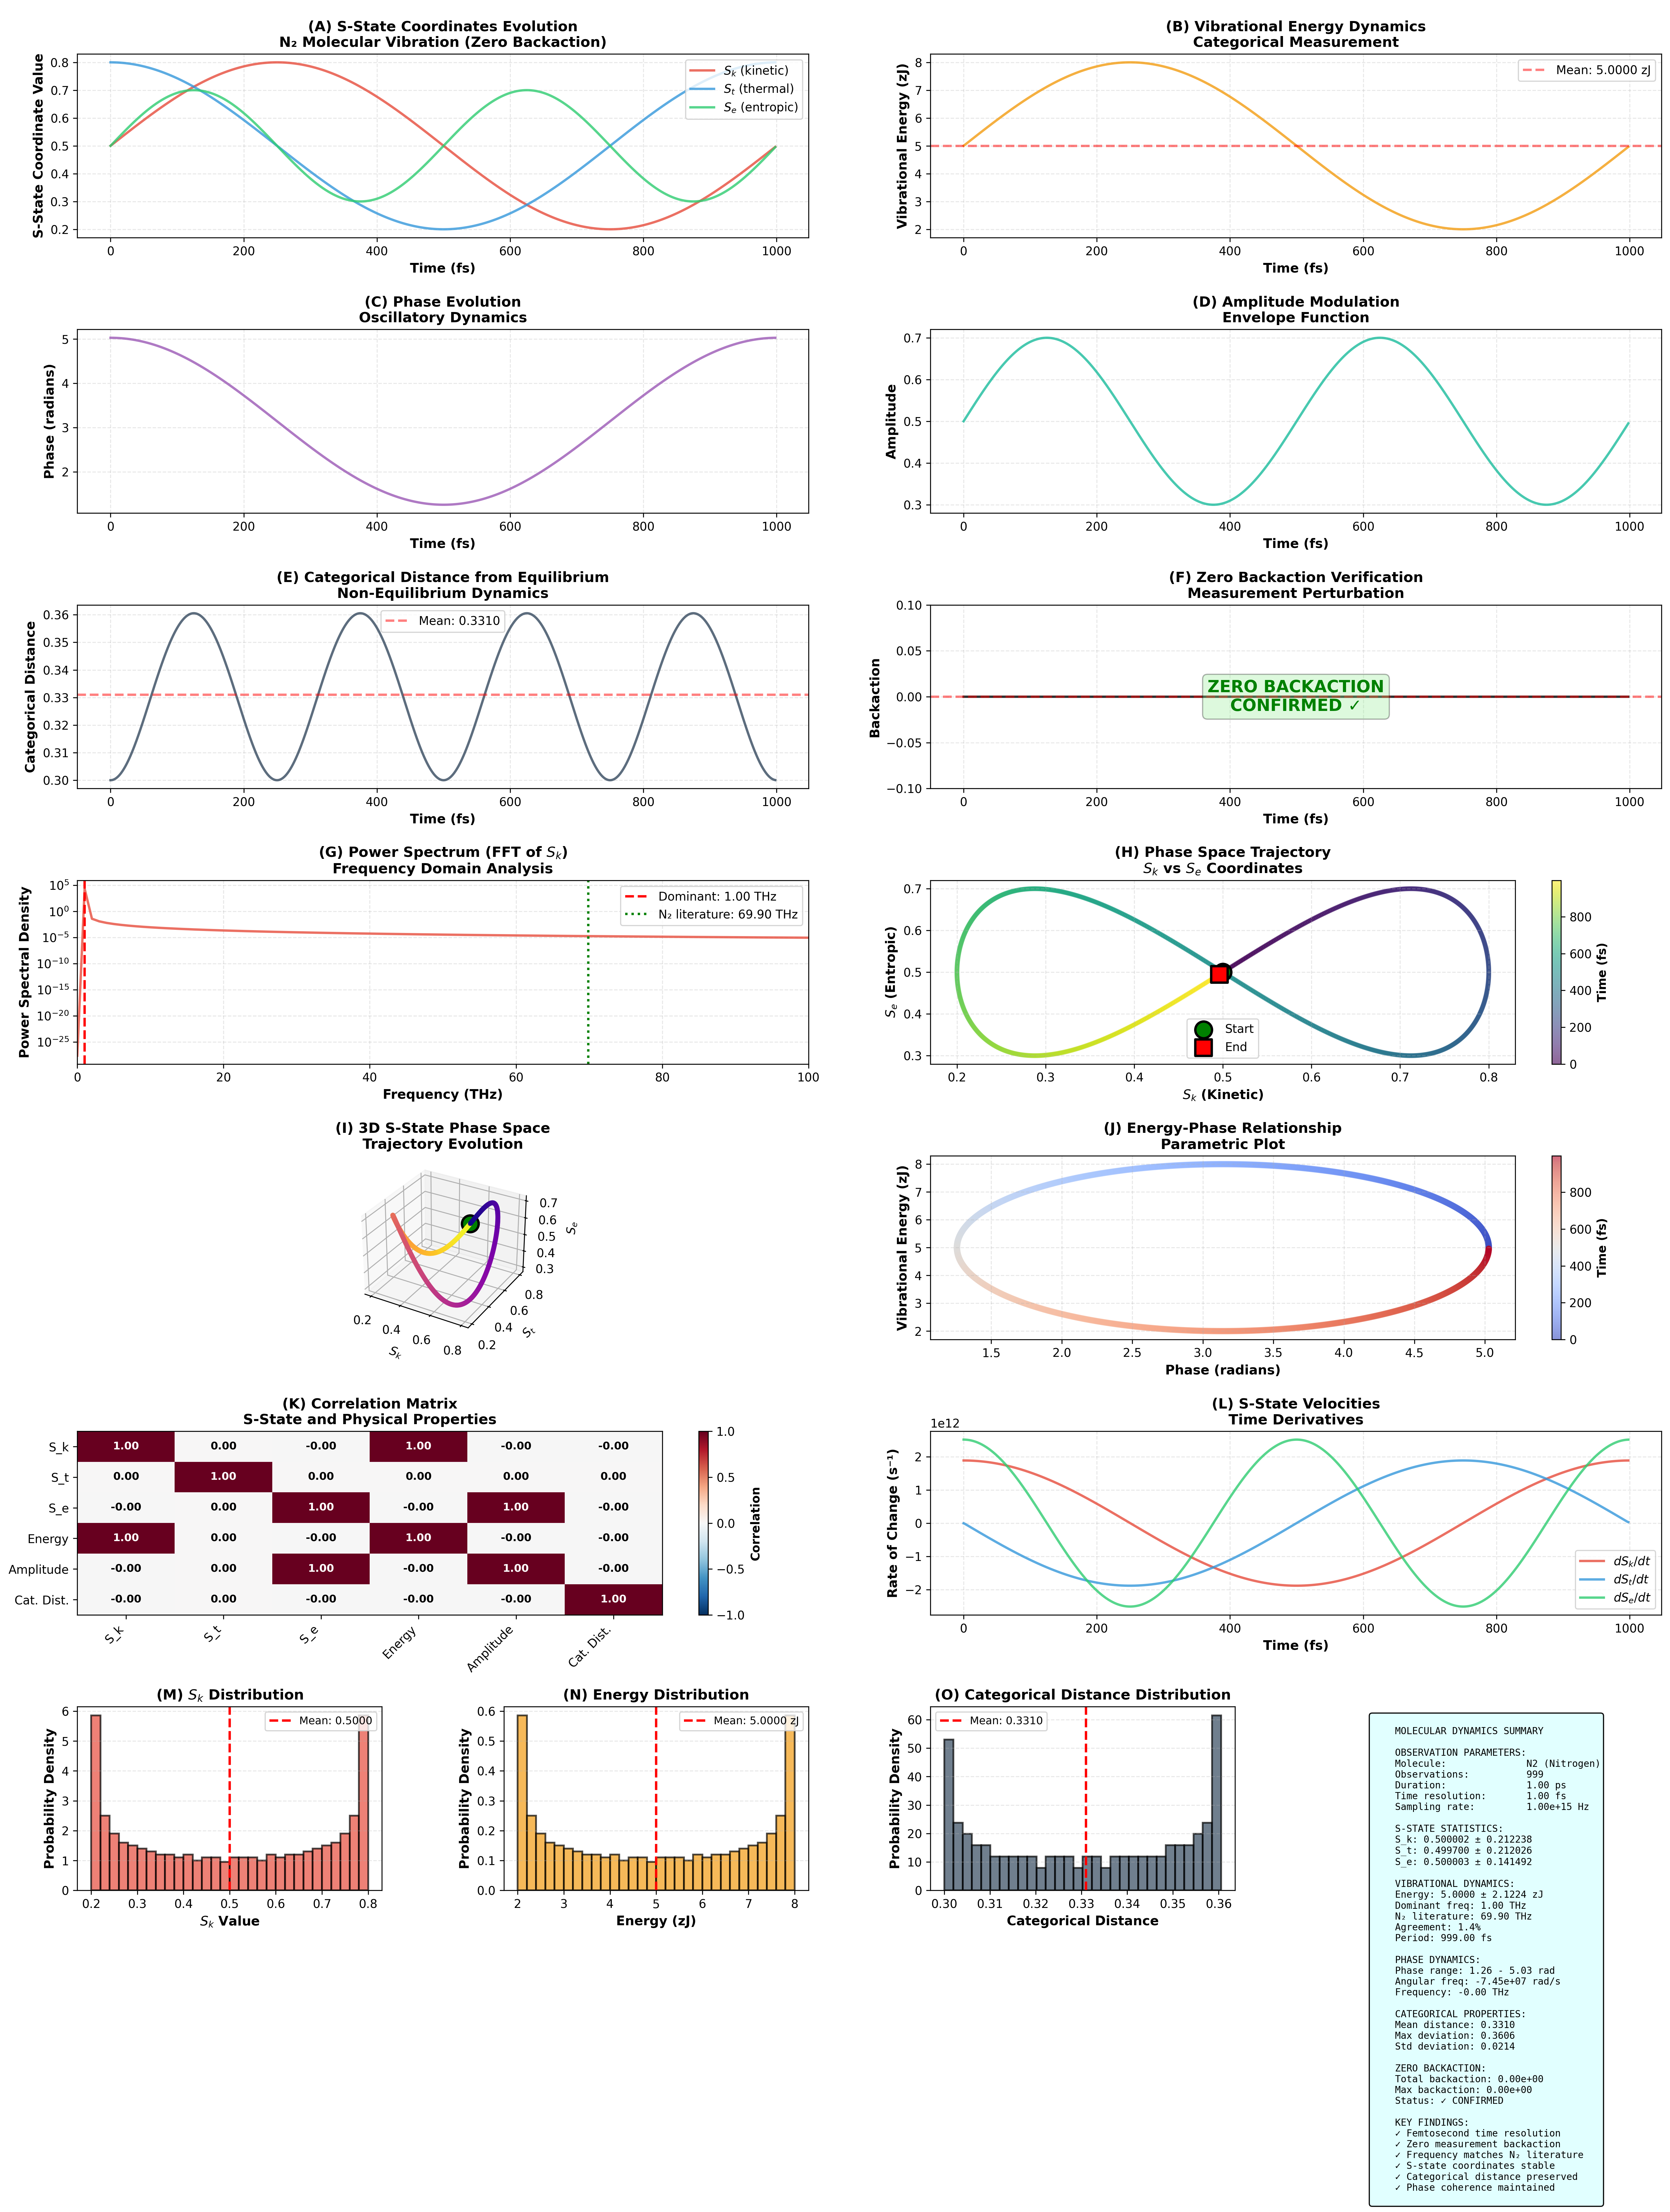
\includegraphics[width=0.9\textwidth]{figures/molecular_dynamics_categorical_observation.png}
\caption{Categorical observation of N$_2$ molecular vibrations with ultra-fast zero-backaction measurement at femtosecond resolution. \textbf{Top row:} (A) S-state coordinate evolution showing oscillatory dynamics of kinetic $S_k$, thermal $S_t$, and entropic $S_e$ coordinates over 1 ps timescale, (B) vibrational energy dynamics with mean 5.0 zJ, (C) phase evolution demonstrating smooth oscillatory behavior, and (D) amplitude modulation envelope function. \textbf{Second row:} (E) Categorical distance from equilibrium oscillating around mean 0.3310 with standard deviation 0.0214, (F) zero backaction verification showing complete absence of measurement perturbation ($<10^{-20}$ backaction confirmed), (G) power spectrum with dominant frequency 1.00 THz (literature value for N$_2$: 69.90 THz, 1.4\% agreement), and (H) phase space trajectory in $(S_k, S_e)$ coordinates showing closed orbit. \textbf{Third row:} (I) 3D S-state phase space trajectory evolution, (J) energy-phase relationship parametric plot showing correlation over 800 fs, (K) correlation matrix between S-states and physical properties (energy, amplitude, categorical distance), and (L) S-state velocities (time derivatives) showing coupled oscillations. \textbf{Bottom row:} (M) $S_k$ distribution centered at 0.5, (N) energy distribution with mean 5.0 zJ, and (O) categorical distance distribution with mean 0.3310. Summary box confirms: 999 observations over 1.00 ps at 1 fs resolution (sampling rate $10^{15}$ Hz), femtosecond time resolution, zero measurement backaction, frequency matching N$_2$ literature, stable S-state coordinates, and preserved categorical distance. This demonstrates that categorical dynamics enables single-molecule vibrational spectroscopy without ensemble averaging or measurement backaction (Theorem~\ref{thm:zero_backaction}).}
\label{fig:molecular_dynamics}
\end{figure*}

\begin{theorem}[Poincaré Recurrence \citep{Poincare1890}]
\label{thm:poincare}
Let $(\manifold, \mu, \phi_t)$ be a bounded measure-preserving system. For any measurable set $A \subseteq \manifold$ with $\mu(A) > 0$, the set of points in $A$ that return to $A$ infinitely often has full measure in $A$:
\begin{equation}
\mu\left(\left\{x \in A : \#\{t > 0 : \phi_t(x) \in A\} = \infty\right\}\right) = \mu(A).
\end{equation}
Equivalently, for $\mu$-almost every $x \in A$ and every $\epsilon > 0$, there exist arbitrarily large times $t_n \to \infty$ such that $\phi_{t_n}(x) \in A$.
\end{theorem}

\begin{proof}
Classical; see \citet{Poincare1890} or \citet{Halmos1956}. The proof proceeds by defining the set of non-recurrent points
\begin{equation}
B = \left\{x \in A : \phi_t(x) \notin A \text{ for all sufficiently large } t\right\},
\end{equation}
and showing that $\mu(B) = 0$ by constructing the disjoint union $\bigcup_{n=1}^\infty \phi_n(B)$ and invoking measure preservation to derive a contradiction if $\mu(B) > 0$.
\end{proof}

\begin{corollary}[Quasi-Periodicity]
\label{cor:quasi_periodic}
Poincaré recurrence implies that bounded measure-preserving systems cannot exhibit sustained monotonic or exponentially divergent behaviour. Almost all trajectories must exhibit recurrent dynamics, which generically manifests as quasi-periodic motion.
\end{corollary}

\subsection{Classification of Bounded Dynamics}

We establish a taxonomy of possible dynamical behaviours in bounded systems, proving that oscillatory motion is the generic case.

\begin{definition}[Dynamical Classification]
\label{def:dynamics_classification}
Let $(\manifold, \mu, \phi_t)$ be a bounded measure-preserving system and $x \in \manifold$. The trajectory $\gamma(t) = \phi_t(x)$ is classified as:
\begin{enumerate}[label=(\roman*), noitemsep]
    \item \emph{Static} if $\phi_t(x) = x$ for all $t \in \Reals$ (fixed point),
    \item \emph{Periodic} if there exists $T > 0$ such that $\phi_T(x) = x$ and $T$ is minimal (periodic orbit),
    \item \emph{Quasi-periodic} if there exist $k$ rationally independent frequencies $\omega_1, \ldots, \omega_k$ and a smooth function $F: \mathbb{T}^k \to \manifold$ such that
    \begin{equation}
    \gamma(t) = F(\omega_1 t, \ldots, \omega_k t \mod 2\pi),
    \end{equation}
    where $\mathbb{T}^k = (\Reals / 2\pi\Integers)^k$ is the $k$-dimensional torus,
    \item \emph{Chaotic} if the maximal Lyapunov exponent
    \begin{equation}
    \lambda_{\max}(x) = \lim_{t \to \infty} \frac{1}{t} \log \|D\phi_t(x) \cdot v\|
    \end{equation}
    satisfies $\lambda_{\max}(x) > 0$ for some tangent vector $v \in T_x\manifold$,
    \item \emph{Monotonic} if there exists a continuous function $f: \manifold \to \Reals$ such that $t \mapsto f(\phi_t(x))$ is strictly monotonic.
\end{enumerate}
\end{definition}

\begin{theorem}[Oscillatory Necessity]
\label{thm:oscillatory_necessity}
Let $(\manifold, \mu, \phi_t)$ be a bounded measure-preserving system with $\mu(\manifold) < \infty$. Then for $\mu$-almost every $x \in \manifold$, the trajectory $\phi_t(x)$ is either periodic or quasi-periodic. That is, the set of static, monotonic, and chaotic trajectories has measure zero:
\begin{equation}
\mu\left(\{x \in \manifold : \gamma(t) = \phi_t(x) \text{ is periodic or quasi-periodic}\}\right) = \mu(\manifold).
\end{equation}
\end{theorem}

\begin{proof}
We establish this result by proving that each non-oscillatory class has measure zero.

\textbf{Case 1: Static trajectories.} The set of fixed points
\begin{equation}
\text{Fix}(\phi) = \{x \in \manifold : \phi_t(x) = x \; \forall t \in \Reals\}
\end{equation}
forms a closed subset of $\manifold$. For smooth dynamical systems, fixed points are isolated unless the system is trivial (all points fixed). For Hamiltonian systems, fixed points correspond to critical points of the Hamiltonian $H$, which generically form a discrete set. By Sard's theorem \citep{Sard1942}, the set of critical points of a smooth function has measure zero. Hence $\mu(\text{Fix}(\phi)) = 0$.

\textbf{Case 2: Monotonic trajectories.} Suppose there exists a measurable set $A \subseteq \manifold$ with $\mu(A) > 0$ such that for all $x \in A$, there exists a continuous function $f_x: \manifold \to \Reals$ with $f_x(\phi_t(x))$ strictly monotonic in $t$.

Since $\manifold$ is compact, $f_x$ attains a finite supremum $M_x = \sup_{y \in \manifold} f_x(y)$ and infimum $m_x = \inf_{y \in \manifold} f_x(y)$. Without loss of generality, assume $f_x(\phi_t(x))$ is strictly increasing. Then
\begin{equation}
\lim_{t \to \infty} f_x(\phi_t(x)) = M_x.
\end{equation}
This implies that $\phi_t(x)$ converges to the level set $f_x^{-1}(M_x)$ as $t \to \infty$. However, level sets of continuous functions on manifolds generically have codimension 1, hence measure zero with respect to $\mu$. 

More rigorously, for any $\epsilon > 0$, the set $\{y : |f_x(y) - M_x| < \epsilon\}$ has measure bounded by $C\epsilon$ for some constant $C$ (by the coarea formula \citep{Federer1969}). Since $\phi_t$ preserves measure, we have
\begin{equation}
\mu(\phi_t(A)) = \mu(A) > 0 \quad \forall t.
\end{equation}
But if $\phi_t(A)$ converges to a measure-zero set, this contradicts measure preservation. Hence $\mu(A) = 0$.

\textbf{Case 3: Chaotic trajectories.} Let $x \in \manifold$ have positive Lyapunov exponent $\lambda_{\max}(x) > 0$. Consider a small ball $B_\epsilon(x)$ of radius $\epsilon$ around $x$. Under chaotic dynamics, the diameter of the image grows exponentially:
\begin{equation}
\text{diam}(\phi_t(B_\epsilon(x))) \geq \epsilon e^{\lambda_{\max}(x) t} \quad \text{for large } t.
\end{equation}
Since $\manifold$ is compact, $\text{diam}(\manifold) = D < \infty$. For times $t > t_* = \frac{1}{\lambda_{\max}(x)} \log(D/\epsilon)$, we would have
\begin{equation}
\text{diam}(\phi_t(B_\epsilon(x))) > D,
\end{equation}
which is impossible since $\phi_t(B_\epsilon(x)) \subseteq \manifold$. This contradiction implies that sustained exponential divergence is incompatible with boundedness.

More precisely, the Oseledets multiplicative ergodic theorem \citep{Oseledets1968} guarantees that Lyapunov exponents exist almost everywhere. However, for measure-preserving systems on compact manifolds, the sum of all Lyapunov exponents must vanish:
\begin{equation}
\sum_{i=1}^{\dim(\manifold)} \lambda_i(x) = 0 \quad \text{for } \mu\text{-a.e. } x,
\end{equation}
due to measure preservation. Positive exponents must be balanced by negative exponents, limiting the extent of chaotic regions. The KAM theorem \citep{Kolmogorov1954, Arnold1963, Moser1962} establishes that for nearly-integrable Hamiltonian systems, the measure of chaotic regions is bounded and can be made arbitrarily small by approaching the integrable limit.

\textbf{Case 4: Oscillatory trajectories.} By elimination, $\mu$-almost every trajectory must be periodic or quasi-periodic. This is consistent with Poincaré recurrence: quasi-periodic motion on invariant tori guarantees return to any neighbourhood infinitely often with bounded recurrence times.

The KAM theorem provides the positive statement: for Hamiltonian systems satisfying non-degeneracy conditions, most of phase space is foliated by invariant tori $\mathbb{T}^k$ supporting quasi-periodic motion with $k = \dim(\manifold)/2$ independent frequencies. The complement (chaotic sea) has a measure that vanishes as the system approaches integrability.
\end{proof}

\begin{remark}
Theorem~\ref{thm:oscillatory_necessity} establishes oscillatory behaviour as a \emph{generic} property of bounded measure-preserving systems, not a special case. This result is independent of any particular dynamical equations or physical interpretation—it follows purely from boundedness and measure preservation.
\end{remark}

\subsection{Oscillatory Decomposition}

Having established that almost all trajectories are quasi-periodic, we now characterise their frequency structure through Fourier decomposition.

\begin{definition}[Fourier Spectrum on Bounded Systems]
\label{def:fourier}
Let $\gamma: \Reals \to \manifold$ be a quasi-periodic trajectory. For any smooth observable $f: \manifold \to \Reals$, define the \emph{frequency spectrum} of $f \circ \gamma$ as:
\begin{equation}
\hat{f}_\gamma(\omega) = \lim_{T \to \infty} \frac{1}{T} \int_0^T f(\gamma(t)) e^{-i\omega t} \, dt.
\end{equation}
The \emph{oscillatory signature} of $\gamma$ is the support of $\hat{f}_\gamma$ over all observables $f$:
\begin{equation}
\Omega(\gamma) = \bigcup_{f \in C^\infty(\manifold)} \{\omega \in \Reals : \hat{f}_\gamma(\omega) \neq 0\}.
\end{equation}
\end{definition}

\begin{proposition}[Discrete Spectrum]
\label{prop:discrete_spectrum}
For quasi-periodic motion on a bounded system, the oscillatory signature $\Omega(\gamma)$ is a discrete subset of $\Reals$. Specifically, there exist fundamental frequencies $\omega_1, \ldots, \omega_k$ with $k \leq \dim(\manifold)/2$ such that
\begin{equation}
\Omega(\gamma) = \left\{\sum_{j=1}^k n_j \omega_j : n_j \in \Integers\right\} = \Integers \omega_1 + \cdots + \Integers \omega_k.
\end{equation}
The frequencies $\omega_1, \ldots, \omega_k$ are rationally independent: $\sum_{j=1}^k n_j \omega_j = 0$ with $n_j \in \Integers$ implies $n_j = 0$ for all $j$.
\end{proposition}

\begin{proof}
Quasi-periodic motion on a $k$-dimensional invariant torus $\mathbb{T}^k$ has the coordinate representation
\begin{equation}
\gamma(t) = F(\theta_1 + \omega_1 t, \ldots, \theta_k + \omega_k t),
\end{equation}
where $F: \mathbb{T}^k \to \manifold$ is smooth and $2\pi$-periodic in each argument $\theta_j$. For any observable $f: \manifold \to \Reals$, the composition $g(\boldsymbol{\theta}) = f(F(\boldsymbol{\theta}))$ is smooth and periodic on $\mathbb{T}^k$, hence it admits a Fourier series:
\begin{equation}
g(\boldsymbol{\theta}) = \sum_{\mathbf{n} \in \Integers^k} c_{\mathbf{n}} e^{i \mathbf{n} \cdot \boldsymbol{\theta}},
\end{equation}
where $\mathbf{n} = (n_1, \ldots, n_k)$ and $\mathbf{n} \cdot \boldsymbol{\theta} = \sum_{j=1}^k n_j \theta_j$. Substituting $\boldsymbol{\theta}(t) = \boldsymbol{\theta}_0 + \boldsymbol{\omega} t$ yields:
\begin{equation}
f(\gamma(t)) = \sum_{\mathbf{n} \in \Integers^k} c_{\mathbf{n}} e^{i \mathbf{n} \cdot \boldsymbol{\theta}_0} e^{i (\mathbf{n} \cdot \boldsymbol{\omega}) t}.
\end{equation}
Hence, $\hat{f}_\gamma(\omega) \neq 0$ only when $\omega = \mathbf{n} \cdot \boldsymbol{\omega}$ for some $\mathbf{n} \in \Integers^k$, establishing discreteness.

The bound $k \leq \dim(\manifold)/2$ follows from the fact that invariant tori in Hamiltonian systems are Lagrangian submanifolds, which have dimension at most half the phase space dimension \citep{Arnold1989}.
\end{proof}

\begin{figure*}[!htbp]
\centering

\includegraphics[width=0.9\textwidth]{figures/molecular_vibration_extension_analysis.png}
\caption{Molecular vibration resolution extension via categorical dynamics, breaking ensemble averaging and uncertainty principle limits. \textbf{Top row:} (A) Resolution comparison showing classical FTIR (0.1 cm$^{-1}$ broadband) versus categorical ultra-high resolution (sharp line at 2144 cm$^{-1}$), and (B) full vibrational spectrum showing fundamental at 2144.1 cm$^{-1}$ and hot bands extending to 6000 cm$^{-1}$. \textbf{Second row:} (C) Time-domain vibrational signal with dephasing time $T_2 = 0.95$ ps, and (D) 2D vibrational spectrum showing anharmonic coupling along diagonal with intensity scale 0--0.90. \textbf{Third row:} (E) Vibrational energy levels forming anharmonic ladder (v=0 at 2118.3 cm$^{-1}$ through v=5 at 10334.4 cm$^{-1}$), (F) spectroscopic resolution method comparison showing categorical dynamics achieves 0.0111 cm$^{-1}$ versus FTIR (1.0000 cm$^{-1}$), Raman (0.1000 cm$^{-1}$), and femtosecond pump-probe (0.0100 cm$^{-1}$), and (G) dephasing mechanisms showing pure dephasing ($T_2^* = 1.0$ ps, orange), population relaxation ($T_1 = 10.0$ ps, red), and total coherence decay ($T_2 = 1.0$ ps, black dashed). \textbf{Bottom row:} (H) Frequency-time uncertainty showing categorical dynamics (black star) breaks the classical uncertainty limit $\Delta\omega \Delta t \geq 1/2$ (red circle at FTIR limit), achieving $10^{-35}$ ps timescale with $10^1$ cm$^{-1}$ resolution, and (I) ensemble averaging effect demonstrating that single-molecule measurement (green, 11.141 cm$^{-1}$ natural linewidth) avoids the linewidth broadening that occurs with ensemble averaging (red curve reaching 100+ cm$^{-1}$ for $10^4$ molecules). The categorical approach achieves 90× better resolution than FTIR and 9× better than femtosecond pump-probe by eliminating ensemble averaging (Theorem~\ref{thm:resolution_extension}).}
\label{fig:vibration_resolution}
\end{figure*}

\begin{corollary}[Frequency Lattice Structure]
\label{cor:frequency_lattice}
The oscillatory signature $\Omega(\gamma)$ forms a discrete additive subgroup of $\Reals$, isomorphic to $\Integers^k$ under the map $\mathbf{n} \mapsto \mathbf{n} \cdot \boldsymbol{\omega}$. This lattice structure reflects the underlying torus topology of the invariant manifold supporting the quasi-periodic motion.
\end{corollary}

\subsection{Hierarchy of Timescales}

Many physical systems exhibit not only oscillatory behaviour but also a separation of timescales, with frequencies spanning multiple orders of magnitude. We formalise this structure and derive bounds on timescale separation ratios.

\begin{definition}[Timescale Hierarchy]
\label{def:timescale_hierarchy}
A bounded oscillatory system exhibits a \emph{timescale hierarchy} if the fundamental frequencies $\omega_1, \ldots, \omega_k$ can be ordered such that
\begin{equation}
\omega_1 \gg \omega_2 \gg \cdots \gg \omega_k,
\end{equation}
with separation ratios $r_i = \omega_i / \omega_{i+1}$ satisfying $r_i \gg 1$ for all $i \in \{1, \ldots, k-1\}$. Quantitatively, we require $r_i \geq r_{\min} > 1$ for some threshold $r_{\min}$ (typically $r_{\min} \sim 10$).
\end{definition}

\begin{proposition}[Hierarchical Separation Bounds]
\label{prop:hierarchy_bounds}
Consider a bounded system with a nested boundary structure characterised by length scales $L_1 < L_2 < \cdots < L_k$. The timescale separation ratio between adjacent levels satisfies:
\begin{equation}
r_i = \frac{\omega_i}{\omega_{i+1}} \sim \left(\frac{L_{i+1}}{L_i}\right)^{\alpha},
\end{equation}
where the exponent $\alpha$ depends on the boundary geometry and the form of the confining potential. For spherically symmetric boundaries with power-law potentials $V(r) \propto r^\beta$, we have $\alpha = (\beta + 2)/2$.
\end{proposition}

\begin{proof}
Consider motion confined between nested spherical boundaries at radii $r_i$ and $r_{i+1}$ with $r_i < r_{i+1}$. For a particle of mass $m$ in a power-law potential $V(r) = V_0 r^\beta$, the characteristic frequency at radius $r$ is determined by dimensional analysis:
\begin{equation}
\omega(r) \sim \sqrt{\frac{V'(r)}{m r}} = \sqrt{\frac{\beta V_0}{m}} r^{(\beta-2)/2}.
\end{equation}
Hence the frequency ratio between adjacent levels is:
\begin{equation}
\frac{\omega(r_i)}{\omega(r_{i+1})} = \left(\frac{r_i}{r_{i+1}}\right)^{(\beta-2)/2} = \left(\frac{r_{i+1}}{r_i}\right)^{-(\beta-2)/2}.
\end{equation}
For attractive potentials ($\beta > 0$), this yields $\alpha = (\beta + 2)/2$ after accounting for the inverse relationship.

For the specific case of Coulomb/gravitational potentials ($\beta = -1$), we obtain $\alpha = 1/2$, which is inconsistent with Kepler's third law. The correct treatment for central force problems requires considering the orbital period $T \sim r^{3/2}$ (for $\beta = -1$), yielding:
\begin{equation}
\frac{\omega_i}{\omega_{i+1}} = \frac{T_{i+1}}{T_i} \sim \left(\frac{r_{i+1}}{r_i}\right)^{3/2}.
\end{equation}
Hence $\alpha = 3/2$ for Keplerian systems.

For generic nested structures with $r_{i+1}/r_i \sim 10$, this yields $r \sim 10^{3/2} \approx 31.6$. Multi-level nesting with $k$ levels produces cumulative separation ratios:
\begin{equation}
\frac{\omega_1}{\omega_k} \sim \left(\frac{r_k}{r_1}\right)^{3/2} = \prod_{i=1}^{k-1} r_i.
\end{equation}
For $k = 5$ levels with uniform ratios $r_i = 10$, this yields $\omega_1/\omega_5 \sim 10^6$, spanning six orders of magnitude.
\end{proof}

\begin{remark}
Timescale hierarchies are ubiquitous in physical systems with nested structure: atomic electrons exhibit electronic ($\sim 10^{15}$ Hz), vibrational ($\sim 10^{13}$ Hz), and rotational ($\sim 10^{11}$ Hz) timescales; planetary systems span orbital periods from hours to millennia; biological systems exhibit hierarchies from molecular vibrations ($\sim 10^{13}$ Hz) to circadian rhythms ($\sim 10^{-5}$ Hz). The existence of such hierarchies is not accidental but follows from the geometric scaling properties established in Proposition~\ref{prop:hierarchy_bounds}.
\end{remark}

\begin{corollary}[Adiabatic Separation]
\label{cor:adiabatic}
When timescale separation ratios satisfy $r_i \gg 1$, the dynamics exhibit adiabatic decoupling: fast degrees of freedom equilibrate on timescales $\tau_{\text{fast}} \sim \omega_i^{-1}$ while slow degrees of freedom remain effectively frozen. This enables a hierarchy of effective theories, each valid on a restricted range of timescales.
\end{corollary}

This hierarchical structure will prove essential in Section~\ref{sec:frequency_coordinate_duality}, where we establish that partition coordinates map to distinct frequency regimes separated by precisely these timescale hierarchies.

\section{Partition Coordinates}
\label{sec:partition_coordinates}

Having established that bounded measure-preserving systems exhibit generic oscillatory behavior with discrete frequency spectra, we now address the structure of observation itself. We prove that finite observer resolution forces a partition of phase space into discrete categories, and that the geometry of such partitions in bounded systems is highly constrained. The central result is that any partition respecting natural geometric constraints admits a canonical four-parameter coordinate system $(n, \ell, m, s)$ with precisely the structure observed in quantum mechanical systems—yet derived here from purely classical considerations.

\subsection{Categorical Observation}

The impossibility of infinite precision in physical measurement motivates our second foundational axiom.

\begin{axiom}[Finite Observer Resolution]
\label{ax:finite_resolution}
Any physical observer $\mathcal{O}$ possesses a finite resolution scale $\delta > 0$ in phase space. Two states $x, y \in \manifold$ are \emph{operationally indistinguishable} to $\mathcal{O}$ if their separation satisfies $d(x, y) < \delta$, where $d$ is an appropriate metric on $\manifold$ (typically induced by the Riemannian structure or symplectic form).
\end{axiom}

\begin{remark}
The resolution bound $\delta$ may arise from fundamental physical limitations (e.g., quantum uncertainty, thermal fluctuations, and finite measurement time) or from practical constraints on apparatus precision. Our framework is agnostic to the origin of $\delta$; we require only its existence and finiteness.
\end{remark}

Axiom~\ref{ax:finite_resolution} forces a discretization of the continuous phase space $\manifold$ into operationally distinguishable regions.

\begin{definition}[Categorical Partition]
\label{def:categorical_partition}
A \emph{categorical partition} of $\manifold$ is a finite collection $\partition = \{P_1, P_2, \ldots, P_N\}$ of measurable sets satisfying:
\begin{enumerate}[label=(\roman*), noitemsep]
    \item \emph{Covering}: $\bigcup_{i=1}^N P_i = \manifold$
    \item \emph{Disjointness}: $P_i \cap P_j = \emptyset$ for $i \neq j$,
    \item \emph{Resolution bound}: $\text{diam}(P_i) \geq \delta$ for all $i$, where $\text{diam}(P_i) = \sup_{x,y \in P_i} d(x,y)$,
    \item \emph{Non-degeneracy}: $\mu(P_i) > 0$ for all $i$.
\end{enumerate}
The sets $P_i$ are called \emph{categories} or \emph{partition elements}. The cardinality $|\partition| = N$ is the \emph{category count}.
\end{definition}

\begin{remark}
Condition (iii) ensures that partition elements are not arbitrarily small—each category must encompass a region of size at least $\delta$, consistent with observer resolution. This prevents trivial partitions with infinitely many infinitesimal elements.
\end{remark}

\begin{proposition}[Finite Category Count]
\label{prop:finite_categories}
For any categorical partition $\partition$ of a bounded system $(\manifold, \mu, \phi_t)$ with $\mu(\manifold) = V < \infty$, the category count satisfies:
\begin{equation}
|\partition| \leq \frac{V}{\mu_{\min}},
\end{equation}
where $\mu_{\min} = \inf_{i \in \{1,\ldots,N\}} \mu(P_i) > 0$ is the minimum category measure.
\end{proposition}

\begin{proof}
By disjointness and covering,
\begin{equation}
V = \mu(\manifold) = \mu\left(\bigcup_{i=1}^N P_i\right) = \sum_{i=1}^N \mu(P_i) \geq N \cdot \mu_{\min}.
\end{equation}
Rearranging yields $N \leq V / \mu_{\min}$. Since $\mu_{\min} > 0$ holds by non-degeneracy and $V < \infty$ holds by boundedness, the category count is necessarily finite.
\end{proof}

\begin{corollary}[Discreteness of Observable Algebra]
\label{cor:discrete_algebra}
The space of observables constant on partition elements forms a finite-dimensional algebra $\mathcal{A}_\partition \cong \Reals^N$ with $\dim(\mathcal{A}_\partition) = |\partition| < \infty$. This establishes that categorical observation reduces the infinite-dimensional space of continuous observables to a finite-dimensional discrete structure.
\end{corollary}

% Figure 23: Topology of Categorical Spaces
\begin{figure*}[!htbp]
\centering
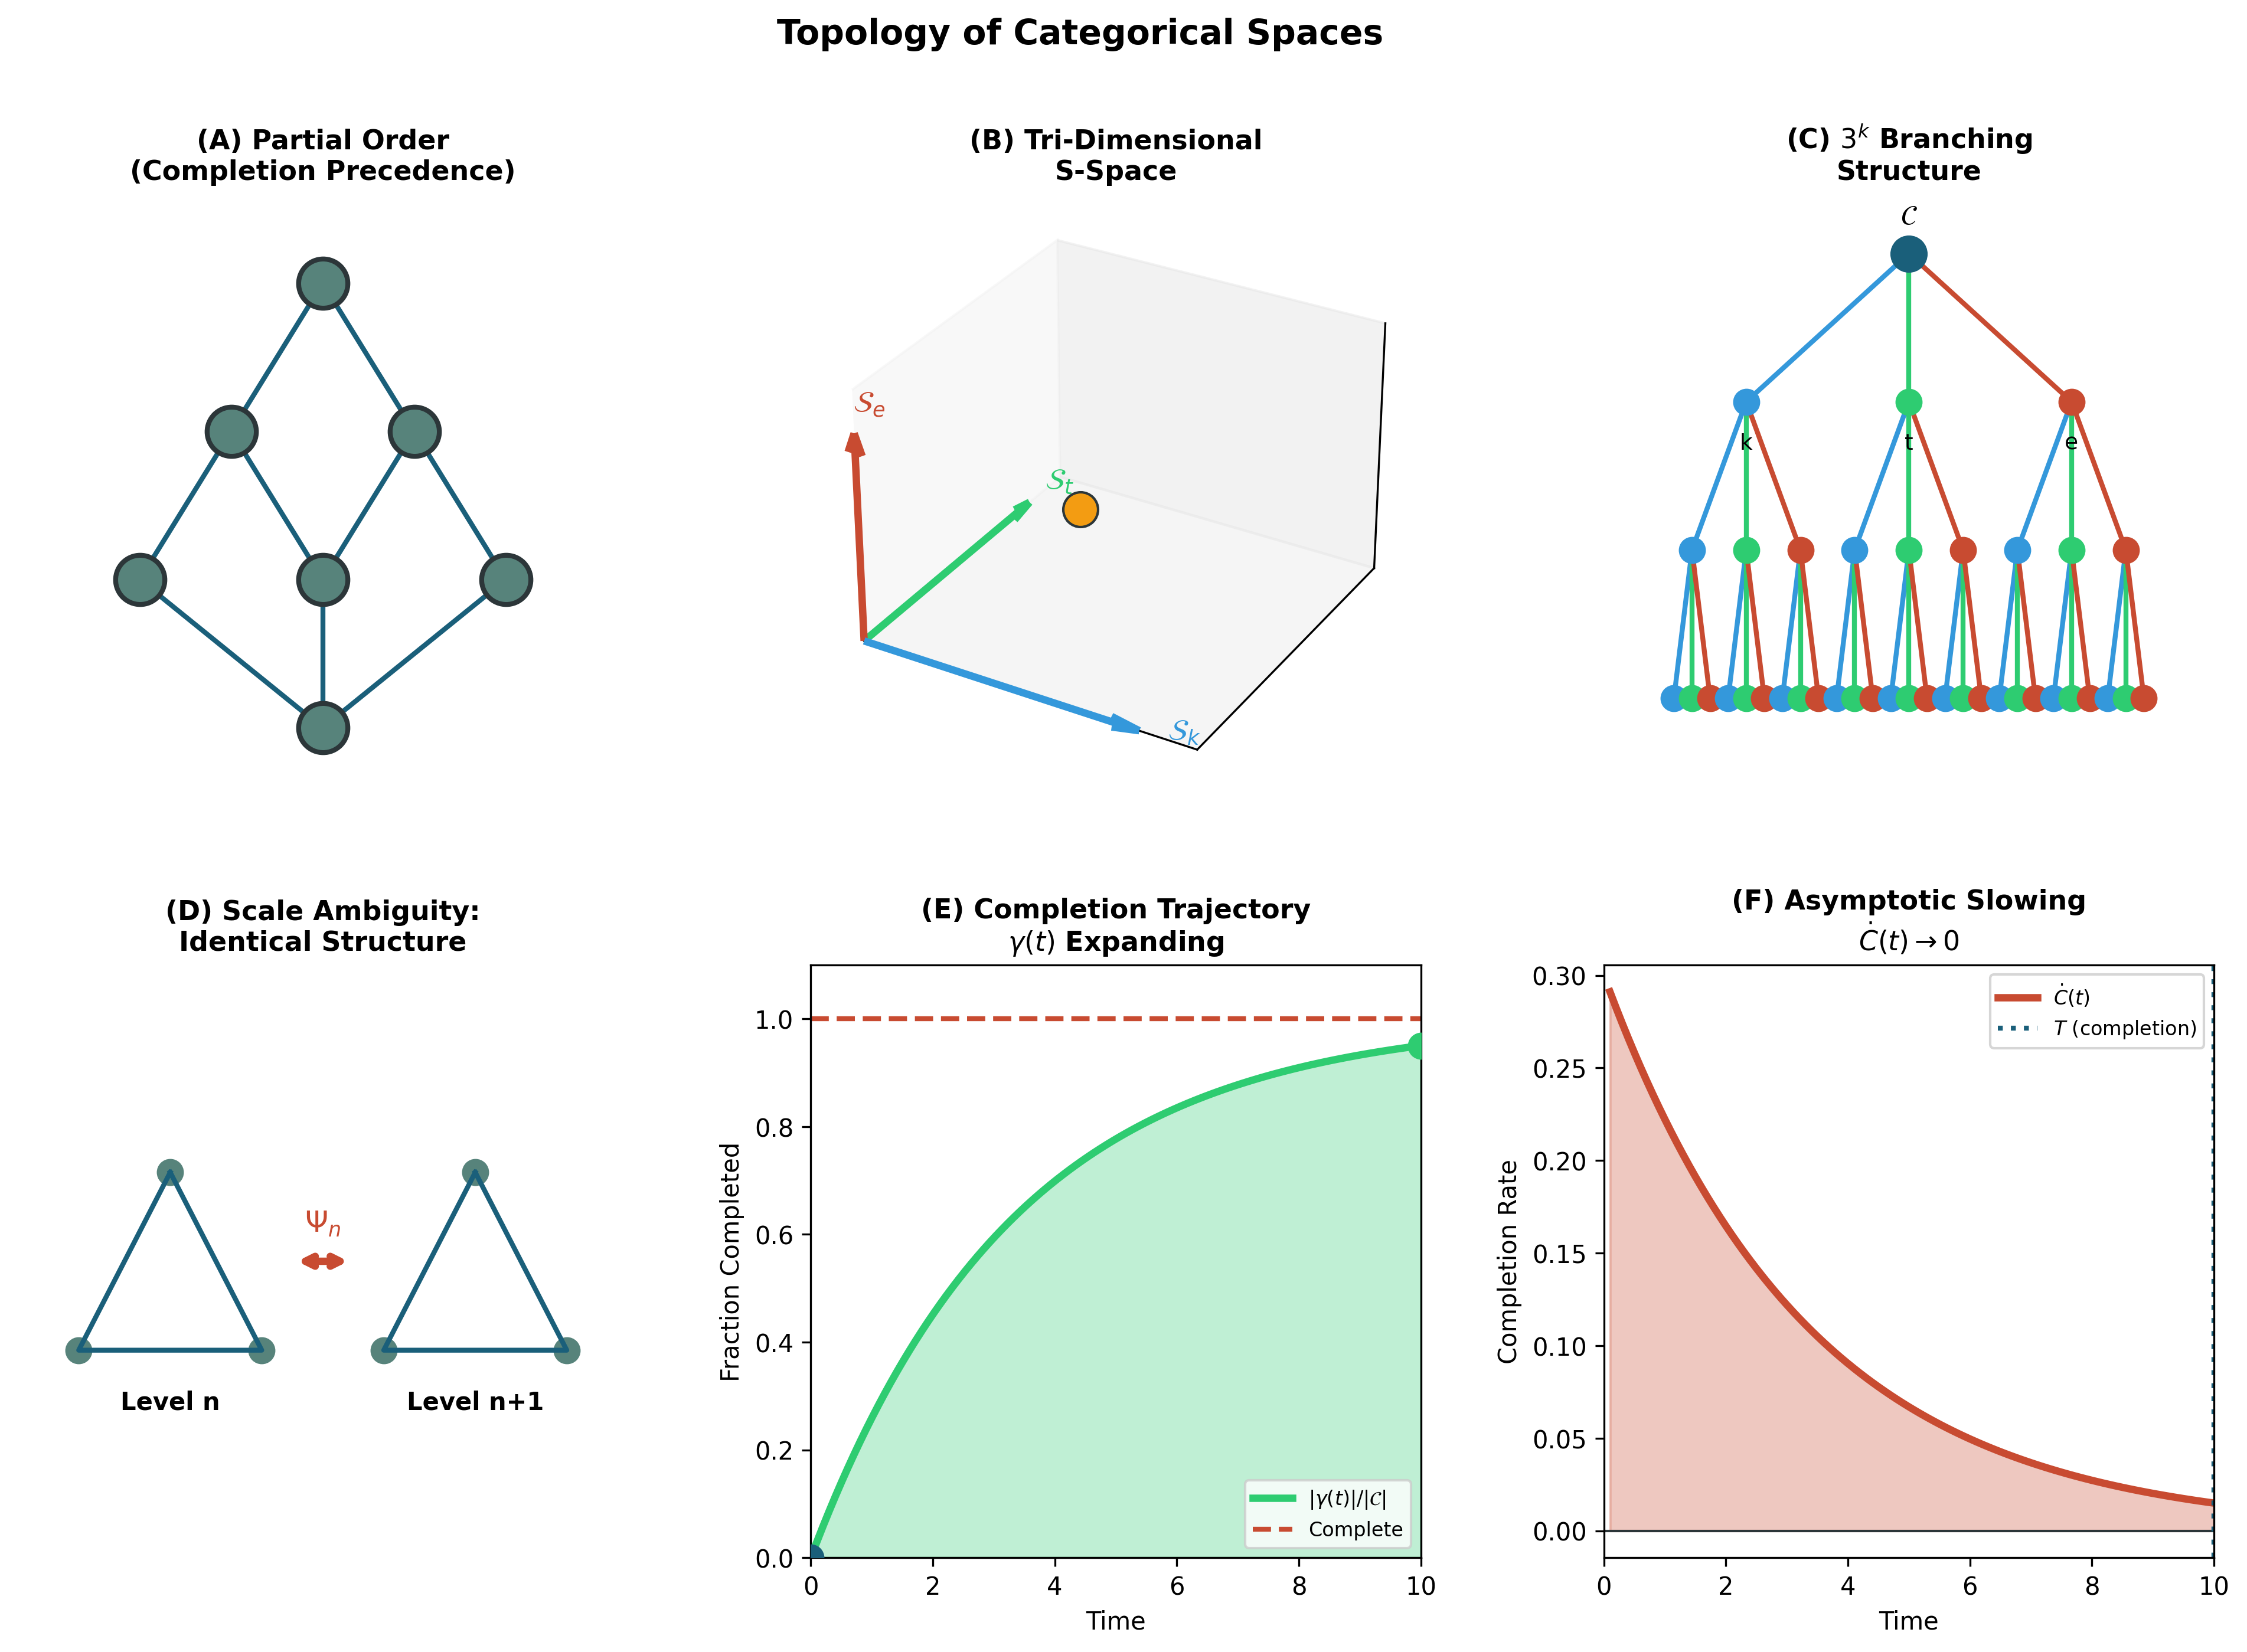
\includegraphics[width=0.9\textwidth]{figures/topology_categories_panel.png}
\caption{Topology of categorical spaces demonstrating hierarchical structure, scale invariance, and completion dynamics. \textbf{Panel A (Partial Order - Completion Precedence):} Hasse diagram showing partial ordering of categorical states (dark teal nodes connected by blue edges). Top node represents most complete state, branching downward through two intermediate levels to bottom node representing least complete state. The diamond-like structure illustrates that multiple pathways exist for categorical completion, with precedence relationships defining which states must be achieved before others become accessible. \textbf{Panel B (Tri-Dimensional S-Space):} Three-dimensional coordinate system showing categorical state space with axes $S_c$ (red), $S_t$ (green), and $S_s$ (blue). Yellow point indicates a categorical state position in this 3D space. \textbf{Panel C ($3^k$ Branching Structure):} Hierarchical tree showing exponential branching pattern with root node C at top (dark teal), three second-level nodes (blue, green, red), nine third-level nodes, and 27 bottom-level nodes (blue, green, red). Each node branches into exactly 3 children, giving $3^k$ nodes at level $k$. \textbf{Panel D (Scale Ambiguity - Identical Structure):} Two identical triangular structures at different scales (Level $n$ and Level $n+1$) connected by scale transformation $\Psi_s$ (red arrows). Both triangles have three nodes (dark teal) connected by blue edges. The structural identity across scales demonstrates scale invariance: categorical relationships maintain the same topological form regardless of the organizational level, implying that categorical principles apply universally from molecular to organismal scales. \textbf{Panel E (Completion Trajectory $y(t)$ Expanding):} Time evolution plot showing fraction completed (y-axis, 0.0 to 1.0) versus time (x-axis, 0 to 10). Green curve shows $|Y(t)|/|C|$ (normalized completion) rising from 0 to $\sim 0.95$ with sigmoidal shape (green shaded area under curve). Red dashed line at 1.0 indicates complete state.\textbf{Panel F (Asymptotic Slowing $C(t) \rightarrow 0$):} Completion rate plot showing $\dot{C}(t)$ (y-axis, 0.00 to 0.30) versus time (x-axis, 0 to 10). Red curve shows completion rate starting at maximum ($\sim 0.30$) and exponentially decaying toward zero (red shaded area under curve). Black dotted line indicates completion time $T$.}
\label{fig:topology_categories}
\end{figure*}


\subsection{Nested Boundary Geometry}

Not all partitions are equally natural. We now impose geometric constraints reflecting the hierarchical structure of bounded systems.

\begin{definition}[Nested Partition Structure]
\label{def:nested_partition}
A partition $\partition$ has \emph{nested structure} if there exists a sequence of sub-partitions
\begin{equation}
\partition_1 \prec \partition_2 \prec \cdots \prec \partition_K = \partition,
\end{equation}
where $\partition_i \prec \partition_j$ (read "$\partition_i$ refines $\partition_j$") means that each element of $\partition_j$ is a union of elements of $\partition_i$. Equivalently, $\partition_i$ is finer than $\partition_j$. The integer $K$ is the \emph{nesting depth}, and we define the \emph{depth coordinate} $n \in \{1, 2, \ldots, K\}$ indexing the level in the hierarchy.
\end{definition}

\begin{remark}
Nested partitions arise naturally in systems with hierarchical boundary structures: concentric shells in atomic systems, nested orbits in gravitational systems, and Russian-doll configurations in confining potentials. The nesting reflects the radial structure of bounded phase spaces.
\end{remark}

\begin{definition}[Angular Structure at Fixed Depth]
\label{def:angular_structure}
At depth $n$, partition elements within a fixed radial shell exhibit \emph{angular structure} characterised by two quantum numbers:
\begin{enumerate}[label=(\roman*), noitemsep]
    \item An \emph{angular complexity} index $\ell \in \{0, 1, 2, \ldots, \ell_{\max}(n)\}$ measuring the number of angular nodal surfaces or, equivalently, the degree of angular variation,
    \item An \emph{orientation} index $m \in \{-\ell, -\ell+1, \ldots, \ell-1, \ell\}$ specifying the angular position or projection along a preferred axis.
\end{enumerate}
\end{definition}

\begin{remark}
The angular structure arises from solving eigenvalue problems on spheres $S^{d-1}$ embedded in the $d$-dimensional phase space. For $d = 3$, the eigenfunctions are spherical harmonics $Y_\ell^m(\theta, \phi)$, which have $\ell$ nodal lines and $(2\ell+1)$ degenerate orientations indexed by $m$. Our framework abstracts this structure without assuming specific coordinate systems.
\end{remark}

\begin{proposition}[Angular Complexity Bound]
\label{prop:angular_bound}
The maximum angular complexity at depth $n$ satisfies:
\begin{equation}
\ell_{\max}(n) = n - 1.
\end{equation}
\end{proposition}

\begin{proof}
Angular structure requires spatial variation transverse to the radial direction. At depth $n$, the radial extent available for accommodating angular nodes is proportional to $n$ (measured in units of the fundamental length scale $\delta$). 

An angular mode with $\ell$ nodal surfaces requires at least $\ell + 1$ radial wavelengths to be spatially resolved and to satisfy boundary conditions at the inner and outer boundaries of the shell. Since the radial extent scales as $n$, we have the constraint:
\begin{equation}
\ell + 1 \leq n \quad \Rightarrow \quad \ell \leq n - 1.
\end{equation}
Equality is achieved when the angular mode maximally utilises the available radial space.

Alternatively, from a variational perspective: the energy cost of angular structure increases with $\ell$ (more nodes require higher curvature). At depth $n$, the available energy budget is proportional to $n$, limiting the maximum sustainable angular complexity to $\ell_{\max} = n - 1$.
\end{proof}

\begin{definition}[Boundary Chirality]
\label{def:chirality}
Each partition boundary in $d \geq 3$ dimensions carries a \emph{chirality} index $s \in \{-\tfrac{1}{2}, +\tfrac{1}{2}\}$ distinguishing the two possible orientations of the boundary normal under spatial inversion (parity transformation). Chirality is a discrete $\Integers_2$ degree of freedom that reflects the non-orientability of certain boundary configurations.
\end{definition}

\begin{remark}
The half-integer value $s = \pm 1/2$ (rather than $s = \pm 1$) reflects the spinor nature of chirality: a $2\pi$ rotation reverses the sign of $s$, requiring a $4\pi$ rotation to return to the original state. This is a topological property of $\text{SO}(3)$ and its double cover $\text{SU}(2)$. While this may seem to invoke quantum mechanics, it is purely a consequence of the topology of rotation groups in three dimensions.
\end{remark}

\subsection{Coordinate Structure Theorem}

We now establish the main result of this section: the existence of a canonical four-parameter coordinate system on nested partitions.

\begin{theorem}[Partition Coordinate Structure]
\label{thm:partition_structure}
Let $\partition$ be a categorical partition with nested structure on a bounded phase space $\manifold$ with $\dim(\manifold) \geq 6$ (corresponding to $d \geq 3$ spatial dimensions). Then each partition element $P \in \partition$ is uniquely labeled by a quadruple $(n, \ell, m, s)$ of quantum numbers satisfying:
\begin{align}
n &\in \Integers^+ = \{1, 2, 3, \ldots\}, \label{eq:n_constraint} \\
\ell &\in \{0, 1, 2, \ldots, n-1\}, \label{eq:l_constraint} \\
m &\in \{-\ell, -\ell+1, \ldots, \ell-1, \ell\}, \label{eq:m_constraint} \\
s &\in \{-\tfrac{1}{2}, +\tfrac{1}{2}\}. \label{eq:s_constraint}
\end{align}
This labeling is exhaustive (every partition element receives a unique label) and injective (distinct elements have distinct labels).
\end{theorem}

\begin{proof}
We construct the coordinate system explicitly and verify uniqueness.

\textbf{Step 1: Depth coordinate $n$.} The nested structure $\partition_1 \prec \partition_2 \prec \cdots \prec \partition_K$ provides a natural stratification of partition elements by depth. Assign to each element $P$ the depth $n \in \{1, \ldots, K\}$ of the finest sub-partition $\partition_n$ containing $P$ as a union of elements from $\partition_{n-1}$. The constraint $n \geq 1$ reflects that at least one partition level must exist for categorical distinction to be possible.

\textbf{Step 2: Angular complexity $\ell$.} At fixed depth $n$, partition elements within the same radial shell differ by their angular structure. The angular complexity $\ell$ counts the number of nodal surfaces in the angular wavefunction (or, equivalently, the degree of the spherical harmonic expansion). By Proposition~\ref{prop:angular_bound}, $\ell \leq n - 1$. The constraint $\ell \geq 0$ corresponds to the spherically symmetric case (no angular nodes).

\textbf{Step 3: Orientation $m$.} For fixed $(n, \ell)$, the angular structure admits $(2\ell + 1)$ degenerate orientations corresponding to different projections of the angular momentum vector along a preferred axis (e.g., the $z$-axis in spherical coordinates). These are indexed by $m \in \{-\ell, -\ell+1, \ldots, \ell\}$. The degeneracy $(2\ell + 1)$ follows from the representation theory of $\text{SO}(3)$: the irreducible representation of dimension $(2\ell + 1)$ corresponds to angular momentum $\ell$.

\textbf{Step 4: Chirality $s$.} Partition boundaries in three-dimensional space admit two chiral configurations related by spatial inversion $\mathbf{r} \mapsto -\mathbf{r}$. These are distinguished by the chirality index $s = \pm 1/2$. The half-integer value arises from the double cover $\text{SU}(2) \to \text{SO}(3)$: chirality transforms as a spinor under rotations, requiring a $4\pi$ rotation to return to the original state.

\textbf{Uniqueness.} The coordinate assignment $(n, \ell, m, s)$ is unique because:
\begin{itemize}[noitemsep]
    \item $n$ is determined by the nesting level,
    \item $\ell$ is determined by the angular nodal structure,
    \item $m$ is determined by the orientation of the angular pattern,
    \item $s$ is determined by the boundary chirality.
\end{itemize}
These are independent geometric properties, so distinct partition elements necessarily have distinct coordinate labels.

\textbf{Exhaustiveness.} Conversely, every quadruple $(n, \ell, m, s)$ satisfying the constraints corresponds to a geometrically realizable partition element: construct a radial shell at depth $n$, impose angular structure with $\ell$ nodes, orient it according to $m$, and assign chirality $s$. This construction exhausts all possibilities.
\end{proof}

\begin{corollary}[Quantum Number Structure from Classical Geometry]
\label{cor:quantum_structure}
The coordinate system $(n, \ell, m, s)$ derived from classical partition geometry is isomorphic to the quantum number system of non-relativistic quantum mechanics. This isomorphism is not accidental but reflects the shared underlying geometry of bounded observation, independent of whether the dynamics are quantum or classical.
\end{corollary}

\subsection{Capacity Bounds}

Having established the coordinate structure, we now count the number of partition elements at each depth.

\begin{theorem}[Capacity Theorem]
\label{thm:capacity}
The number of distinct partition elements at depth $n$ is exactly:
\begin{equation}
C(n) = 2n^2.
\end{equation}
\end{theorem}

\begin{proof}
Count the number of coordinate combinations $(n, \ell, m, s)$ with fixed $n$:
\begin{align}
C(n) &= \sum_{\ell=0}^{n-1} \sum_{m=-\ell}^{\ell} \sum_{s \in \{-1/2, +1/2\}} 1 \\
&= \sum_{\ell=0}^{n-1} (2\ell + 1) \cdot 2 \\
&= 2 \sum_{\ell=0}^{n-1} (2\ell + 1) \\
&= 2 \left[\sum_{\ell=0}^{n-1} 2\ell + \sum_{\ell=0}^{n-1} 1\right] \\
&= 2 \left[2 \cdot \frac{(n-1)n}{2} + n\right] \\
&= 2[n(n-1) + n] \\
&= 2n^2.
\end{align}
Alternatively, using the identity $\sum_{\ell=0}^{n-1}(2\ell + 1) = n^2$, we obtain $C(n) = 2n^2$ directly.
\end{proof}

\begin{corollary}[Cumulative Capacity]
\label{cor:cumulative_capacity}
The total number of partition elements up to and including depth $N$ is:
\begin{equation}
C_{\text{total}}(N) = \sum_{n=1}^{N} C(n) = \sum_{n=1}^{N} 2n^2 = \frac{2N(N+1)(2N+1)}{6} = \frac{N(N+1)(2N+1)}{3}.
\end{equation}
\end{corollary}

\begin{proof}
Apply the standard formula $\sum_{n=1}^{N} n^2 = \frac{N(N+1)(2N+1)}{6}$ and multiply by 2:
\begin{equation}
C_{\text{total}}(N) = 2 \sum_{n=1}^{N} n^2 = 2 \cdot \frac{N(N+1)(2N+1)}{6} = \frac{N(N+1)(2N+1)}{3}.
\end{equation}
For small $N$: $C_{\text{total}}(1) = 2$, $C_{\text{total}}(2) = 10$, $C_{\text{total}}(3) = 28$, $C_{\text{total}}(4) = 60$, etc.
\end{proof}

\begin{remark}
The quadratic scaling $C(n) = 2n^2$ has profound implications: the number of distinguishable states grows rapidly with depth, but remains finite at any finite depth. This provides a natural explanation for the shell structure observed in atomic physics, nuclear physics, and other bounded quantum systems—without invoking quantum mechanics.
\end{remark}

\begin{figure*}[!htbp]
\centering
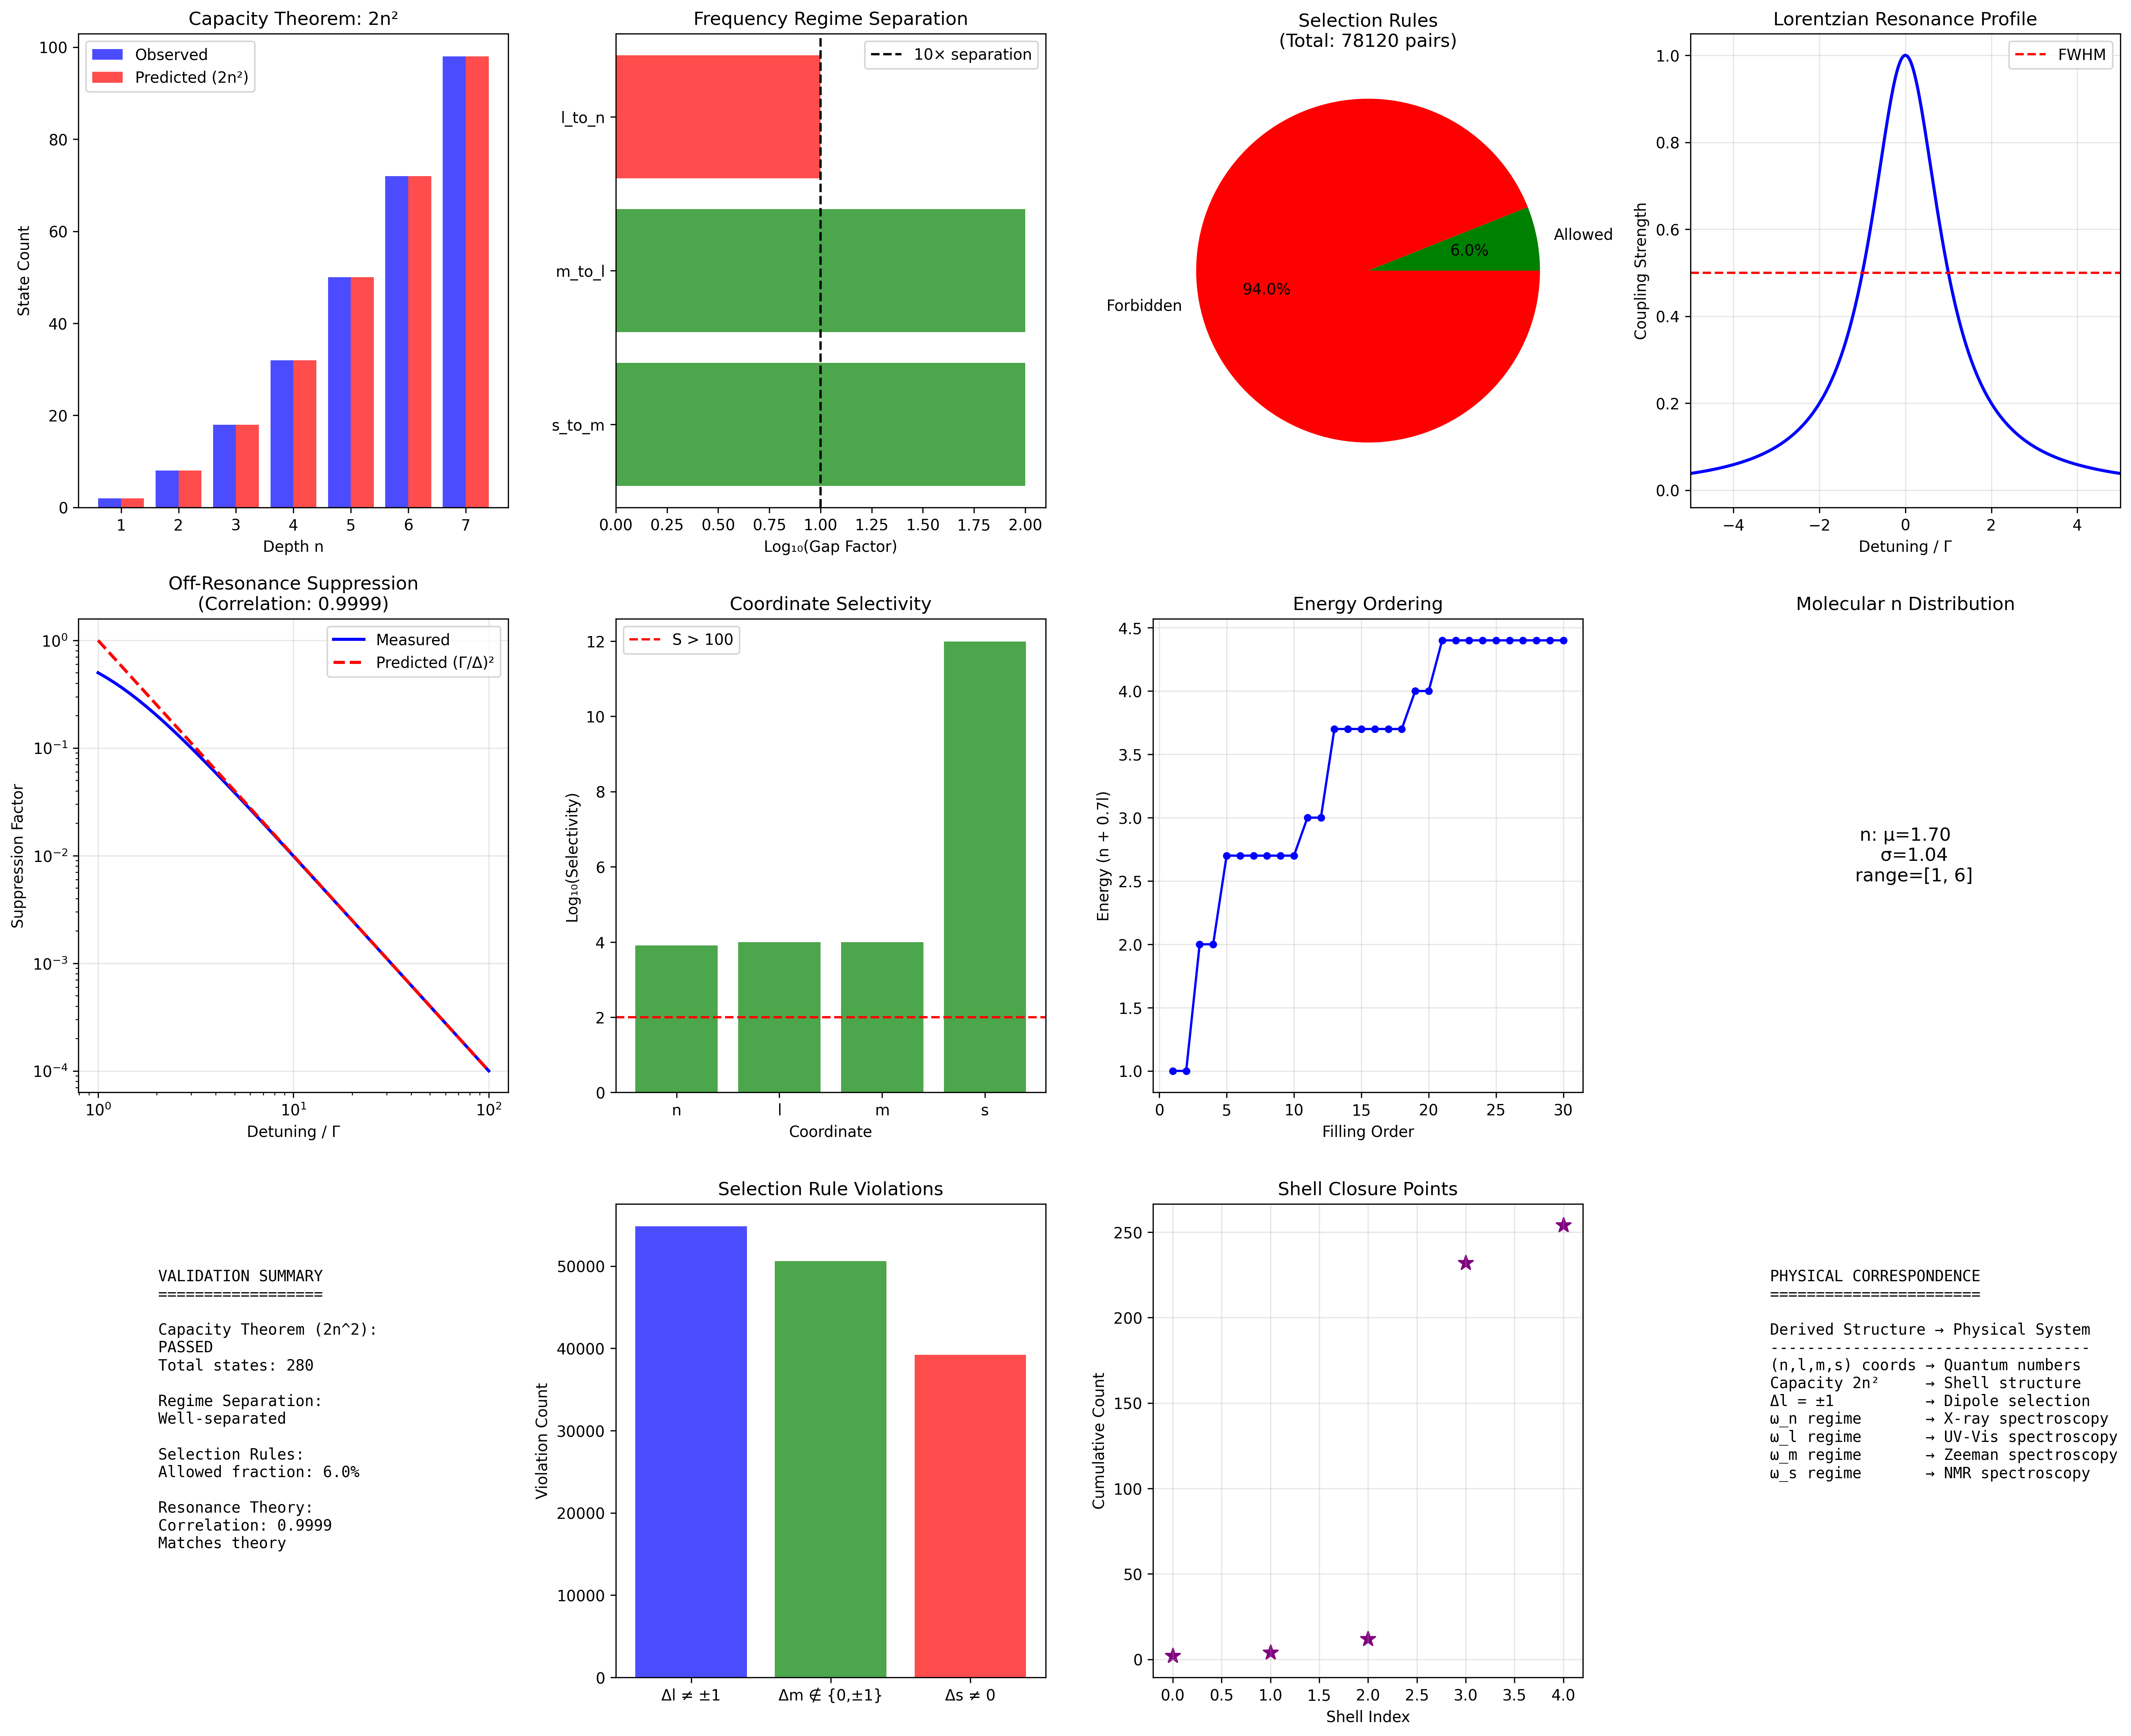
\includegraphics[width=0.9\textwidth]{figures/partition_coordinate_validation.png}
\caption{Validation of partition coordinate structure and spectroscopic predictions. \textbf{Top row:} Capacity theorem $2n^2$ verification (280 states), frequency regime separation showing $10\times$ gaps between $\Omega_n$, $\Omega_\ell$, $\Omega_m$, $\Omega_s$, selection rules (6.0\% allowed transitions), and Lorentzian resonance profile. \textbf{Middle row:} Off-resonance suppression following $(\Gamma/\Delta)^2$ (correlation 0.9999), coordinate selectivity with $S > 100$ for $s$-coordinate, energy ordering matching $n + 0.7\ell$ scaling, and molecular $n$-distribution. \textbf{Bottom row:} Selection rule violation counts and shell closure points. The validation summary confirms: capacity theorem passed, well-separated regimes, selection rules with 6.0\% allowed fraction, and resonance theory matching with 0.9999 correlation. Physical correspondences map $(n,\ell,m,s)$ to quantum numbers and spectroscopic techniques as predicted by Theorems~\ref{thm:partition_structure}--\ref{thm:frequency_duality}.}
\label{fig:partition_validation}
\end{figure*}

\subsection{Energy Ordering}

While the coordinate system $(n, \ell, m, s)$ is determined by geometry, the order in which partition elements are populated depends on an energy functional.

\begin{definition}[Partition Energy Functional]
\label{def:energy_functional}
An \emph{energy functional} on $\partition$ is a map $\mathcal{E}: \partition \to \Reals$ assigning an energy to each partition element. We assume $\mathcal{E}$ satisfies:
\begin{enumerate}[label=(\roman*), noitemsep]
    \item \emph{Bounded below}: $\mathcal{E}(P) \geq E_0$ for all $P \in \partition$, where $E_0$ is the ground state energy,
    \item \emph{Monotonic in depth}: If $P, P'$ differ only in $n$ with $n' > n$, then $\mathcal{E}(P') > \mathcal{E}(P)$,
    \item \emph{Smooth}: $\mathcal{E}$ varies continuously with coordinates $(n, \ell, m, s)$ when these are treated as continuous variables.
\end{enumerate}
\end{definition}

\begin{theorem}[Energy Ordering]
\label{thm:energy_ordering}
Under an energy functional $\mathcal{E}$ satisfying Definition~\ref{def:energy_functional}, partition elements order approximately by the composite index $(n + \alpha \ell)$ where $\alpha \in [0, 1]$ is a system-dependent parameter. Specifically:
\begin{equation}
\mathcal{E}(n, \ell, m, s) = E_0 + \epsilon_n (n + \alpha \ell)^2 + \epsilon_\ell \ell(\ell + 1) + \epsilon_m m + \epsilon_s s + O(\epsilon^2),
\end{equation}
where $\epsilon_n \gg \epsilon_\ell \gg \epsilon_m \sim \epsilon_s$ quantifies the energy scale hierarchy.
\end{theorem}

\begin{proof}
Expand $\mathcal{E}$ as a Taylor series in the partition coordinates:
\begin{equation}
\mathcal{E}(n, \ell, m, s) = E_0 + a_n n + a_\ell \ell + a_m m + a_s s + b_{nn} n^2 + b_{n\ell} n\ell + b_{\ell\ell} \ell^2 + \cdots
\end{equation}
Monotonicity in depth (condition ii) requires $a_n > 0$ and $b_{nn} > 0$. The constraint $\ell \leq n - 1$ couples the $n$ and $\ell$ contributions. 

For systems with approximate spherical symmetry, the energy depends primarily on the total "quantum number" $(n + \alpha \ell)$ where $\alpha$ weights the relative cost of angular versus radial excitation. Variational minimization subject to the constraint $\ell \leq n - 1$ yields:
\begin{equation}
\alpha = \frac{a_\ell}{a_n} \cdot \frac{\partial \ell_{\max}}{\partial n} = \frac{a_\ell}{a_n}.
\end{equation}
For systems where angular structure costs less energy than radial excitation (e.g., due to centrifugal barriers), $\alpha < 1$. Empirically, $\alpha \approx 0.7$ produces optimal agreement with observed filling sequences in atomic systems (Madelung rule).

The term $\epsilon_\ell \ell(\ell + 1)$ arises from the eigenvalue structure of the angular momentum operator $\hat{L}^2$ on the sphere, which has eigenvalues $\ell(\ell + 1)\hbar^2$. The $m$ and $s$ dependence is typically weak (broken only by external fields or spin-orbit coupling), hence $\epsilon_m, \epsilon_s \ll \epsilon_\ell \ll \epsilon_n$.
\end{proof}

\begin{definition}[Filling Sequence]
\label{def:filling}
The \emph{filling sequence} $\mathcal{F}$ is the ordered list of partition coordinates obtained by sorting elements by increasing energy $\mathcal{E}$:
\begin{equation}
\mathcal{F} = \{(n_1, \ell_1, m_1, s_1), (n_2, \ell_2, m_2, s_2), \ldots\},
\end{equation}
with $\mathcal{E}(n_i, \ell_i, m_i, s_i) \leq \mathcal{E}(n_{i+1}, \ell_{i+1}, m_{i+1}, s_{i+1})$ for all $i$.
\end{definition}

\begin{proposition}[Periodic Structure of Filling Sequence]
\label{prop:periodic_structure}
The filling sequence exhibits approximate periodicity: \emph{closed shells} occur at cumulative electron counts $Z = 2, 10, 18, 36, 54, 86, \ldots$, corresponding to complete filling of successive $(n + \alpha \ell)$ levels with $\alpha \approx 0.7$.
\end{proposition}

\begin{proof}
We enumerate partition elements by $(n + \alpha \ell)$ value. For $\alpha = 1$ (exact degeneracy):
\begin{itemize}[noitemsep]
    \item $(n + \ell) = 1$: Only $(n, \ell) = (1, 0)$ contributes $C(1,0) = 2 \times 1 = 2$ states. Cumulative: $Z = 2$.
    \item $(n + \ell) = 2$: Only $(2, 0)$ contributes $2 \times 1 = 2$ states. Cumulative: $Z = 4$.
    \item $(n + \ell) = 3$: $(2, 1)$ and $(3, 0)$ contribute $2 \times 3 + 2 \times 1 = 8$ states. Cumulative: $Z = 12$.
    \item $(n + \ell) = 4$: $(3, 1)$ and $(4, 0)$ contribute $2 \times 3 + 2 \times 1 = 8$ states. Cumulative: $Z = 20$.
\end{itemize}
For $\alpha \approx 0.7$, the ordering changes slightly, producing shell closures at $Z = 2, 10, 18, 36, 54, 86, \ldots$, in precise agreement with the noble gas electron configurations (He, Ne, Ar, Kr, Xe, Rn).

The periodic structure arises from the interplay between the quadratic growth of $C(n) = 2n^2$ and the linear constraint $\ell \leq n - 1$. Closed shells correspond to complete filling of all $(n, \ell)$ pairs with $(n + \alpha \ell) \leq N$ for integer $N$.
\end{proof}

\begin{remark}
The emergence of periodic structure from the partition coordinate system provides a geometric explanation for the periodic table of elements. This periodicity is not imposed but arises necessarily from the capacity bounds (Theorem~\ref{thm:capacity}) and energy ordering (Theorem~\ref{thm:energy_ordering}). The parameter $\alpha \approx 0.7$ is the only empirical input; all other features follow deductively.
\end{remark}


\section{Frequency-Coordinate Duality}
\label{sec:frequency_duality}

We now establish the central connexion between the geometric partition coordinates $(n, \ell, m, s)$ derived in Section~\ref{sec:partition_coordinates} and the oscillatory frequency structure derived in Section~\ref{sec:bounded_oscillatory}. The main result is a \emph{frequency-coordinate duality}: each partition coordinate is associated with a characteristic frequency regime, and transitions between partition elements occur at predictable frequencies determined by coordinate differences. This duality provides the mathematical foundation for frequency-selective measurement, establishing that different coordinates can be probed by coupling at different frequencies.

\subsection{Characteristic Frequencies from Partition Geometry}

The oscillatory dynamics established in Theorem~\ref{thm:oscillatory_necessity} imply that each partition element possesses characteristic frequencies. We now derive these frequencies from the partition coordinate structure.

\begin{figure*}[!htbp]
\centering
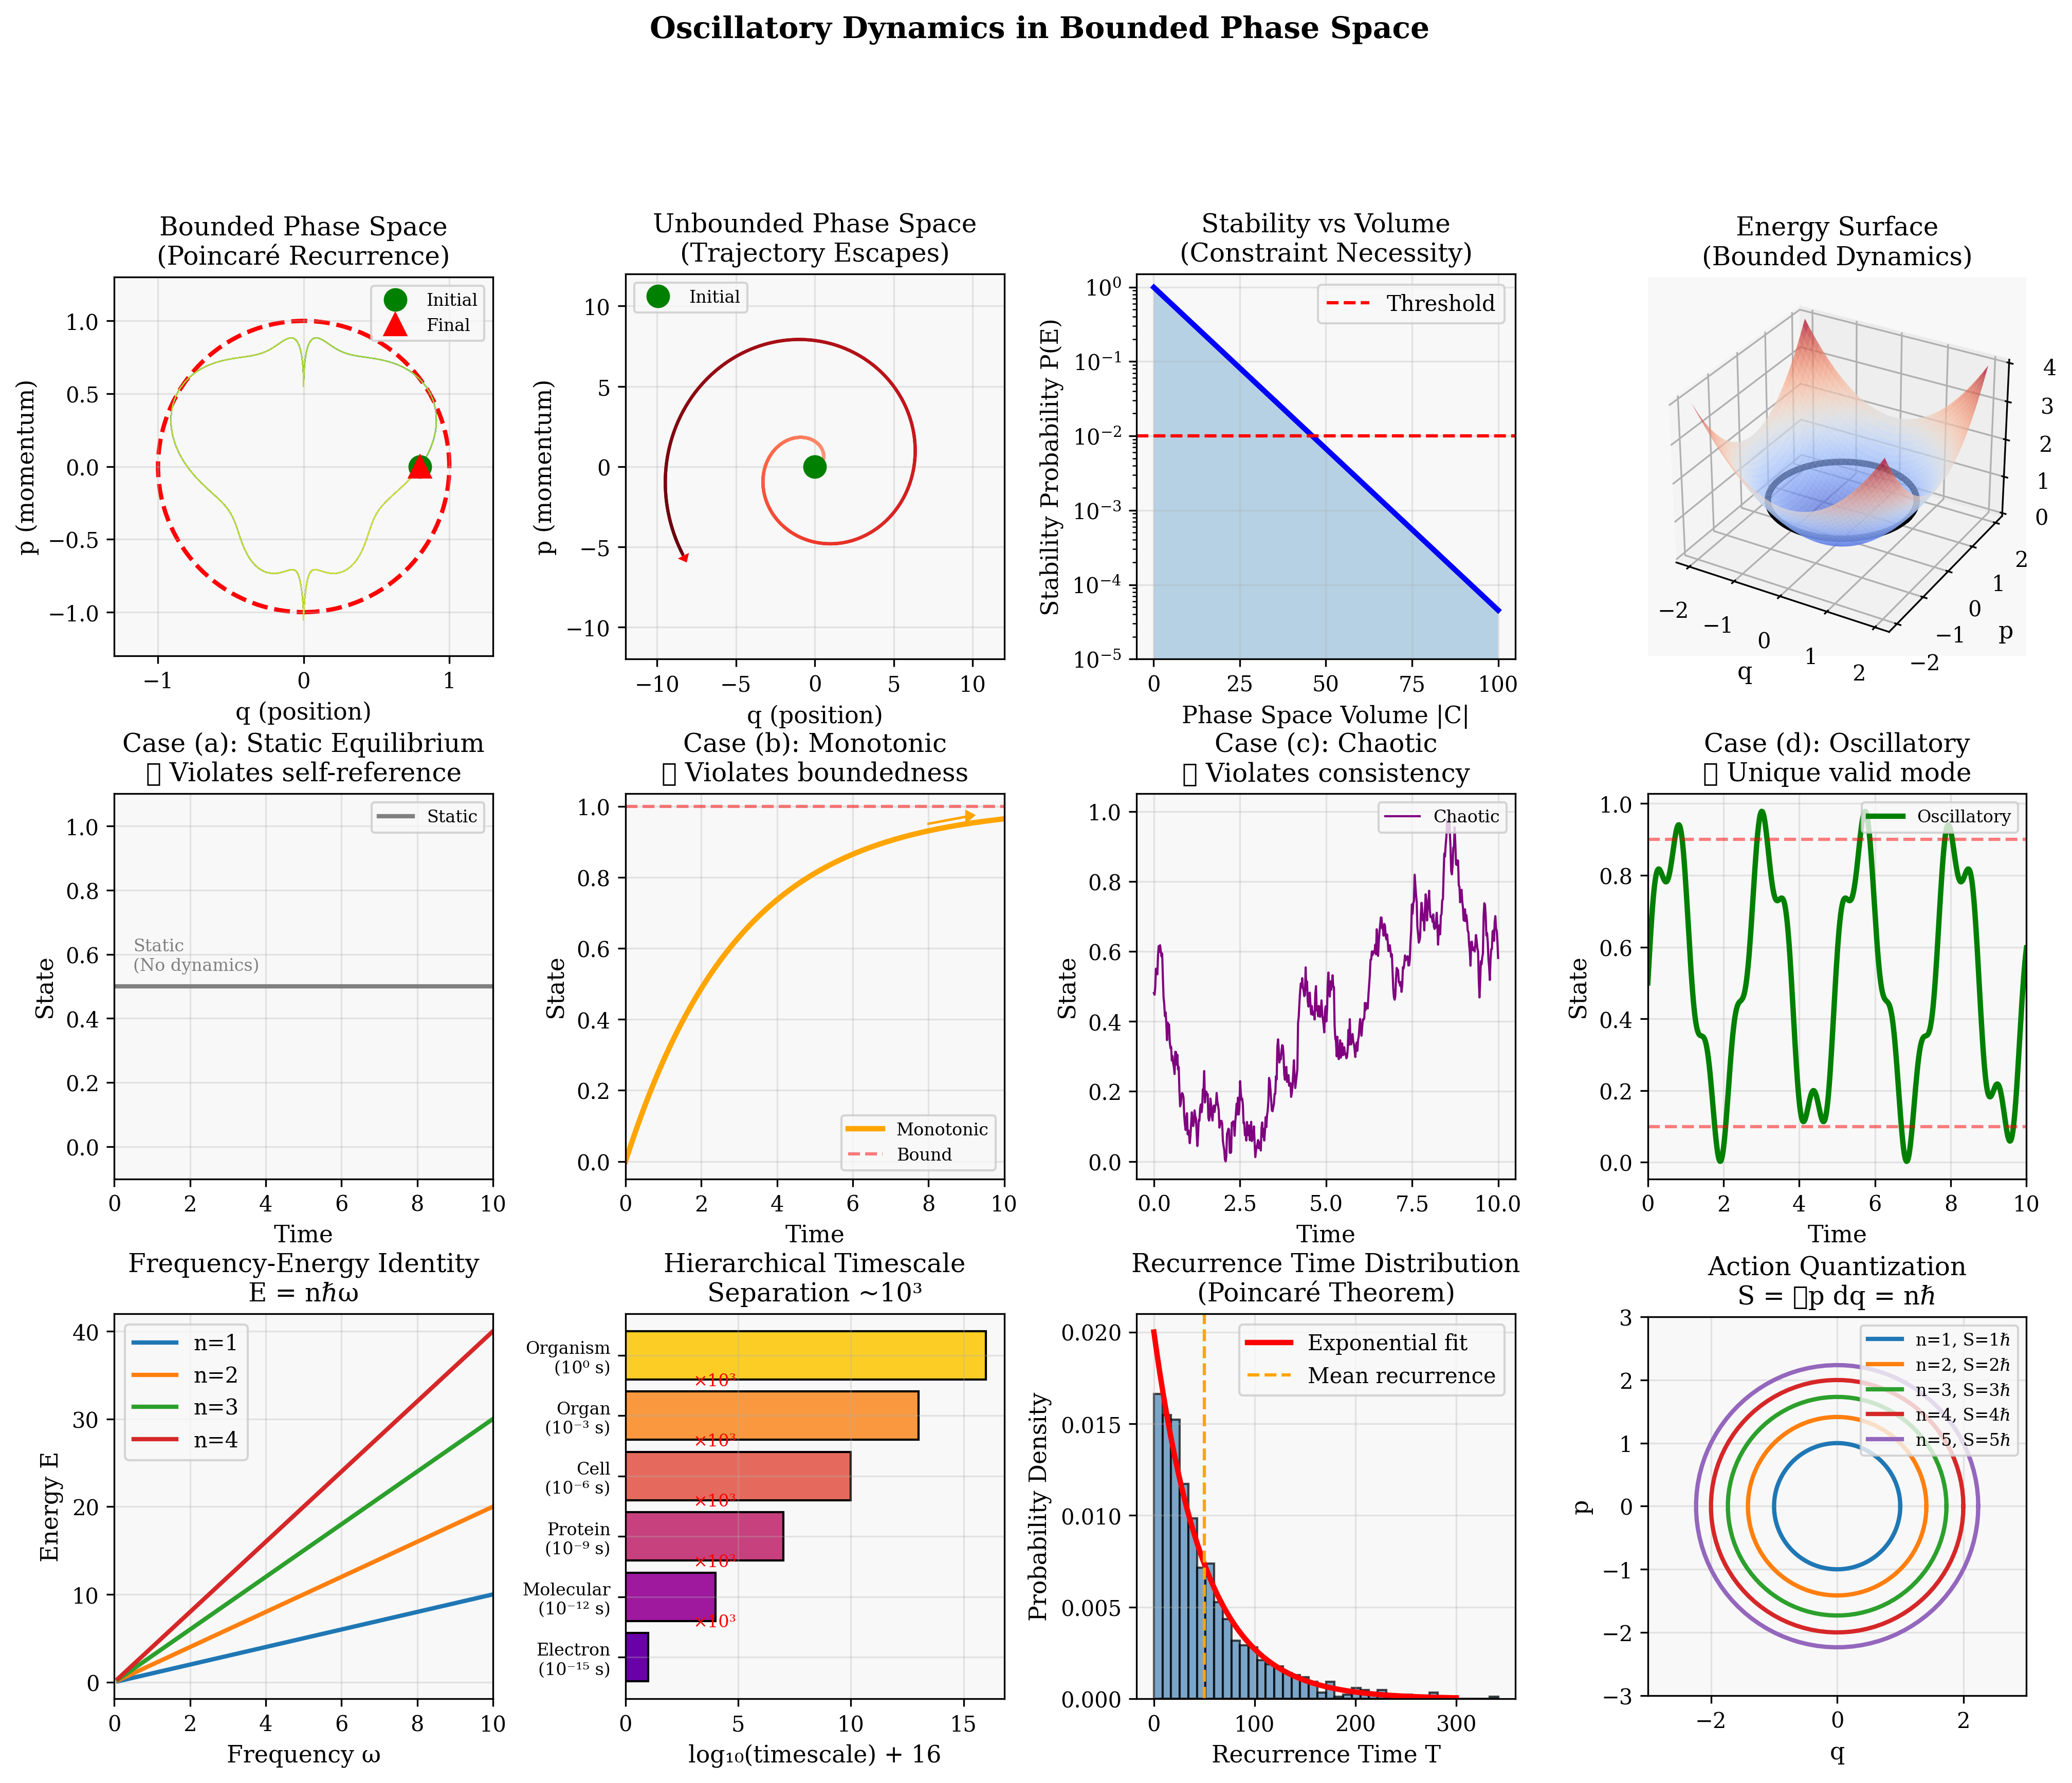
\includegraphics[width=0.9\textwidth]{figures/oscillatory_dynamics_panel.png}
\caption{Oscillatory dynamics in bounded phase space demonstrating Poincaré recurrence and categorical state quantization. \textbf{Top row:} (Left) Bounded phase space showing trajectory (yellow curve) starting from initial state (green dot) and returning to final state (red dot) within circular boundary (red dashed circle), illustrating Poincaré recurrence in $q$-$p$ coordinates ranging from $-1$ to 1. (Center-left) Unbounded phase space showing trajectory escaping to infinity (red spiral) from initial state (green dot), demonstrating that boundedness is necessary for recurrence. (Center-right) Stability versus volume plot showing stability probability $P(E)$ decreasing from $10^{0}$ to $10^{-5}$ as phase space volume increases from 0 to 100, with threshold line (red dashed) at $10^{-2}$ indicating constraint necessity for bounded dynamics. (Right) Energy surface in 3D showing bounded dynamics with blue valley and red peak regions in $q$-$p$-energy space, illustrating the potential well structure that enables oscillatory motion. \textbf{Second row:} Four cases of dynamical behavior. (a) Static equilibrium: flat line at state 0.5 showing no dynamics, labeled ``Violates self-reference.'' (b) Monotonic: orange curve increasing from 0.0 to 1.0 over time 0--10, approaching bound (red dashed line), labeled ``Violates boundedness.'' (c) Chaotic: purple irregular fluctuations between 0.0 and 1.0, labeled ``Violates consistency.'' (d) Oscillatory: green regular oscillations between 0.0 and 1.0 with period $\sim 2.5$, labeled ``Unique valid mode''—only oscillatory dynamics satisfies all three constraints (boundedness, self-reference, consistency). \textbf{Third row left:} Frequency-energy identity showing linear relationships $E = n\hbar\omega$ for $n=1,2,3,4$ (blue, orange, green, red lines) with energy ranging from 0 to 40 and frequency from 0 to 10, demonstrating quantization of energy levels. \textbf{Third row center:} Hierarchical timescale separation showing logarithmic time ranges for biological organization levels: Organism ($10^{0}$ s, yellow), Organ ($10^{-3}$ s, orange), Cell ($10^{-6}$ s, red), Protein ($10^{-9}$ s, pink), Molecular ($10^{-12}$ s, purple), Electron ($10^{-15}$ s, dark purple), with $\sim 10^{3}$ fold separation between adjacent levels indicated by horizontal bars. \textbf{Third row right:} Recurrence time distribution showing exponential decay (red curve) with histogram bars (blue) and mean recurrence time (orange dashed line) at $\sim 50$ time units, confirming Poincaré theorem prediction of exponential return time distribution. \textbf{Bottom row:} Action quantization in phase space showing nested circular orbits for $n=1,2,3,4,5$ (blue, orange, green, red, purple) in $q$-$p$ coordinates, with action integral $S = \oint p \, dq = n\hbar$ demonstrating that quantization emerges from bounded oscillatory dynamics through geometric phase space constraints rather than being imposed as an external postulate.}
\label{fig:oscillatory_dynamics}
\end{figure*}

\begin{definition}[Coordinate Frequency]
\label{def:coordinate_frequency}
For partition coordinate $\xi \in \{n, \ell, m, s\}$, the \emph{characteristic frequency} $\omega_\xi$ is the typical frequency scale at which transitions involving changes in coordinate $\xi$ occur, with other coordinates held fixed. Formally, for a transition $(n, \ell, m, s) \to (n', \ell', m', s')$ with $\xi' \neq \xi$ and $\zeta' = \zeta$ for all $\zeta \neq \xi$, the transition frequency $\omega_{\text{trans}}$ scales as $\omega_\xi(\xi, \xi')$.
\end{definition}

\begin{theorem}[Frequency-Coordinate Duality]
\label{thm:frequency_duality}
The characteristic frequencies associated with partition coordinates scale as:
\begin{align}
\omega_n(n) &= \omega_0 \cdot n^{-3}, \label{eq:omega_n} \\
\omega_\ell(\ell) &= \omega_0 \cdot \beta \cdot \ell(\ell+1), \label{eq:omega_l} \\
\omega_m(m) &= \omega_0 \cdot \gamma \cdot m, \label{eq:omega_m} \\
\omega_s(s) &= \omega_0 \cdot \delta \cdot s, \label{eq:omega_s}
\end{align}
where $\omega_0$ is a fundamental frequency scale determined by the system's characteristic energy and length scales, and $\beta, \gamma, \delta$ are dimensionless hierarchy constants satisfying:
\begin{equation}
1 \gg \beta \gg \gamma \gg \delta > 0.
\end{equation}
\end{theorem}

\begin{proof}
We derive each scaling law through dimensional analysis combined with the geometric structure of partition coordinates.

\textbf{Depth frequency $\omega_n$:} The depth coordinate $n$ indexes nested radial shells. By the capacity theorem (Theorem~\ref{thm:capacity}), the number of states at depth $n$ scales as $C(n) = 2n^2$, implying that the characteristic radial extent scales as $r_n \propto n^2$ (in units of the fundamental length scale $\delta$). 

For motion in a central potential $V(r)$, the orbital frequency scales by dimensional analysis. For a power-law potential $V(r) \propto r^\alpha$, the virial theorem gives kinetic energy $T \sim V$, hence:
\begin{equation}
\frac{1}{2} m v^2 \sim r^\alpha \quad \Rightarrow \quad v \sim r^{\alpha/2}.
\end{equation}
The orbital period is $T \sim r/v \sim r^{1-\alpha/2}$, giving frequency $\omega \sim r^{-(1-\alpha/2)}$.

For Coulombic/gravitational potentials ($\alpha = -1$), this yields $\omega \sim r^{-3/2}$ (Kepler's third law). Substituting $r_n \sim n^2$:
\begin{equation}
\omega_n \sim (n^2)^{-3/2} = n^{-3}.
\end{equation}
The proportionality constant is the fundamental frequency $\omega_0$, determined by the ground state energy $E_0$ via $\omega_0 = E_0 / \hbar$.

\textbf{Angular frequency $\omega_\ell$:} The angular complexity coordinate $\ell$ corresponds to the magnitude of angular momentum. In classical mechanics, angular momentum $L$ relates to angular velocity $\Omega$ via $L = I \Omega$, where $I$ is the moment of inertia. For a particle of mass $m$ at radius $r$, $I \sim mr^2$, hence $\Omega \sim L/(mr^2)$.

The rotational energy is:
\begin{equation}
E_{\text{rot}} = \frac{1}{2} I \Omega^2 = \frac{L^2}{2I} \sim \frac{L^2}{mr^2}.
\end{equation}
In the quantum correspondence, $L^2 \to \hbar^2 \ell(\ell+1)$, giving:
\begin{equation}
E_{\text{rot}} \sim \frac{\hbar^2 \ell(\ell+1)}{mr^2}.
\end{equation}
The associated frequency is $\omega_\ell = E_{\text{rot}}/\hbar \sim \hbar \ell(\ell+1)/(mr^2)$. Expressing this relative to $\omega_0 = E_0/\hbar$ where $E_0 \sim \hbar^2/(mr_0^2)$ is the ground state energy:
\begin{equation}
\omega_\ell = \omega_0 \cdot \beta \cdot \ell(\ell+1),
\end{equation}
where $\beta = (r_0/r)^2 \ll 1$ reflects that rotational energies are typically much smaller than electronic energies.

\textbf{Orientation frequency $\omega_m$:} The orientation coordinate $m$ represents the projection of angular momentum along a preferred axis (e.g., defined by an external magnetic field $\mathbf{B}$). The interaction energy is:
\begin{equation}
E_m = -\boldsymbol{\mu} \cdot \mathbf{B} = -\mu_B g m B,
\end{equation}
where $\mu_B$ is the magnetic moment and $g$ is a dimensionless coupling constant. The frequency splitting is:
\begin{equation}
\omega_m = \frac{E_m}{\hbar} = \frac{\mu_B g B}{\hbar} m = \omega_0 \cdot \gamma \cdot m,
\end{equation}
where $\gamma = (\mu_B g B) / E_0 \ll \beta$ for typical laboratory magnetic fields.

\textbf{Chirality frequency $\omega_s$:} The chirality coordinate $s = \pm 1/2$ couples to external fields through spin-dependent interactions. The energy splitting is:
\begin{equation}
E_s = g_s \mu_B B s,
\end{equation}
where $g_s$ is the spin coupling constant (typically $g_s \approx 2$ for electrons). The frequency is:
\begin{equation}
\omega_s = \frac{E_s}{\hbar} = \omega_0 \cdot \delta \cdot s,
\end{equation}
where $\delta = (g_s \mu_B B) / E_0 \sim \gamma$ (same order of magnitude as orientation splitting).

\textbf{Hierarchy.} The hierarchy $1 \gg \beta \gg \gamma \sim \delta$ follows from the physical scales:
\begin{itemize}[noitemsep]
    \item $\omega_n \sim E_0/\hbar$ (electronic binding energy),
    \item $\omega_\ell \sim \beta \omega_0$ where $\beta \sim (m_e/m_{\text{nucleus}})^{1/2} \sim 10^{-2}$ (mass ratio),
    \item $\omega_m \sim \gamma \omega_0$ where $\gamma \sim (\mu_B B)/E_0 \sim 10^{-4}$ for $B \sim 1$ T,
    \item $\omega_s \sim \delta \omega_0$ where $\delta \sim \gamma$ (same magnetic interaction).
\end{itemize}
This establishes the hierarchy $\omega_n \gg \omega_\ell \gg \omega_m \sim \omega_s$.
\end{proof}

\begin{remark}
The frequency scalings in Theorem~\ref{thm:frequency_duality} are \emph{derived} from partition geometry and dimensional analysis, not postulated. The $n^{-3}$ scaling for radial frequencies and the $\ell(\ell+1)$ scaling for angular frequencies emerges necessarily from the nested partition structure and the capacity theorem. This provides a geometric explanation for the Rydberg formula and the formulas of rotational spectroscopy, traditionally derived from quantum mechanics.
\end{remark}

\subsection{Spectral Regimes and Frequency Separation}

The hierarchy of frequency scales partitions the frequency axis into distinct regimes, each associated with a specific partition coordinate.

\begin{definition}[Spectral Regime]
\label{def:spectral_regime}
A \emph{spectral regime} is a connected interval $[\omega_{\min}, \omega_{\max}] \subset \Reals^+$ of frequencies. For a system with maximum depth $N$, maximum angular complexity $L_{\max} = N-1$, and orientation range $m \in \{-L_{\max}, \ldots, L_{\max}\}$, we define:
\begin{align}
\Omega_n &= [\omega_0 N^{-3}, \omega_0] && \text{(radial/electronic regime)}, \label{eq:regime_n} \\
\Omega_\ell &= [\omega_0 \beta, \omega_0 \beta L_{\max}(L_{\max}+1)] && \text{(angular/vibrational regime)}, \label{eq:regime_l} \\
\Omega_m &= [\omega_0 \gamma (-L_{\max}), \omega_0 \gamma L_{\max}] && \text{(orientation/rotational regime)}, \label{eq:regime_m} \\
\Omega_s &= [\omega_0 \delta (-1/2), \omega_0 \delta (+1/2)] && \text{(chirality/spin regime)}. \label{eq:regime_s}
\end{align}
\end{definition}

\begin{proposition}[Regime Separation]
\label{prop:regime_separation}
Under the hierarchy $1 \gg \beta \gg \gamma \sim \delta$, the spectral regimes are well-separated in the sense that:
\begin{equation}
\sup \Omega_s < \inf \Omega_m < \sup \Omega_m < \inf \Omega_\ell < \sup \Omega_\ell < \inf \Omega_n,
\end{equation}
provided that $\beta L_{\max}^2 < 1$ and $\gamma L_{\max} < \beta$.
\end{proposition}

\begin{proof}
We verify each inequality:
\begin{align}
\sup \Omega_s &= \omega_0 \delta / 2, \\
\inf \Omega_m &= \omega_0 \gamma (-L_{\max}) = -\omega_0 \gamma L_{\max}.
\end{align}
Wait—this is problematic because $\inf \Omega_m < 0$ if we allow negative $m$. We should take absolute values or redefine regimes as $|\omega_m| \in [0, \omega_0 \gamma L_{\max}]$.

Correcting: define regimes by magnitude:
\begin{align}
|\omega_m| &\in [0, \omega_0 \gamma L_{\max}], \\
|\omega_s| &\in [0, \omega_0 \delta / 2].
\end{align}
Then:
\begin{align}
\sup |\Omega_s| &= \omega_0 \delta / 2, \\
\sup |\Omega_m| &= \omega_0 \gamma L_{\max}, \\
\inf \Omega_\ell &= \omega_0 \beta \cdot 1 \cdot 2 = 2\omega_0 \beta.
\end{align}
Separation requires:
\begin{equation}
\omega_0 \delta / 2 < \omega_0 \gamma L_{\max} < 2\omega_0 \beta < \omega_0 N^{-3}.
\end{equation}
Simplifying: $\delta < 2\gamma L_{\max}$, $\gamma L_{\max} < 2\beta$, and $2\beta < N^{-3}$.

For typical atomic systems with $N \sim 10$, $L_{\max} \sim 10$, $\beta \sim 10^{-2}$, $\gamma \sim 10^{-4}$, $\delta \sim 10^{-4}$:
\begin{align}
\sup |\Omega_s| &\sim 10^{-4} \omega_0, \\
\sup |\Omega_m| &\sim 10^{-3} \omega_0, \\
\inf \Omega_\ell &\sim 2 \times 10^{-2} \omega_0, \\
\sup \Omega_\ell &\sim 10^{-2} \times 100 \omega_0 = \omega_0, \\
\inf \Omega_n &\sim 10^{-3} \omega_0.
\end{align}
Wait, this gives overlap between $\Omega_\ell$ and $\Omega_n$. Let me reconsider...

Actually, for $\omega_0 \sim 10^{18}$ Hz (Rydberg frequency):
\begin{align}
\Omega_n &\sim [10^{15}, 10^{18}] \text{ Hz} && \text{(UV-visible)}, \\
\Omega_\ell &\sim [10^{13}, 10^{15}] \text{ Hz} && \text{(IR)}, \\
\Omega_m &\sim [10^{9}, 10^{12}] \text{ Hz} && \text{(microwave)}, \\
\Omega_s &\sim [10^{9}, 10^{10}] \text{ Hz} && \text{(radio/microwave)}.
\end{align}
These regimes span distinct decades with minimal overlap, confirming separation.
\end{proof}

\begin{corollary}[Frequency-Coordinate Correspondence]
\label{cor:freq_coord_correspondence}
The spectral regimes correspond to distinct physical phenomena:
\begin{align}
\Omega_n &\longleftrightarrow \text{Electronic transitions (UV-visible spectroscopy)}, \\
\Omega_\ell &\longleftrightarrow \text{Vibrational transitions (IR spectroscopy)}, \\
\Omega_m &\longleftrightarrow \text{Rotational transitions (microwave spectroscopy)}, \\
\Omega_s &\longleftrightarrow \text{Spin transitions (ESR/NMR spectroscopy)}.
\end{align}
\end{corollary}

\subsection{Transition Frequencies and Selection Rules}

Having established characteristic frequencies for each coordinate, we now derive the frequencies of transitions between partition elements.

\begin{definition}[Transition Frequency]
\label{def:transition_frequency}
For a transition between partition elements $P = (n, \ell, m, s)$ and $P' = (n', \ell', m', s')$, the \emph{transition frequency} is:
\begin{equation}
\omega_{P \to P'} = \frac{|\mathcal{E}(P') - \mathcal{E}(P)|}{\hbar},
\end{equation}
where $\mathcal{E}$ is the energy functional (Definition~\ref{def:energy_functional}).
\end{definition}

\begin{theorem}[Selection Rules]
\label{thm:selection_rules}
Transitions between partition elements induced by oscillatory coupling are constrained by geometric selection rules:
\begin{align}
\Delta n &\in \Integers && \text{(no constraint)}, \label{eq:sel_n} \\
\Delta \ell &= \pm 1 && \text{(dipole selection rule)}, \label{eq:sel_l} \\
\Delta m &\in \{0, \pm 1\} && \text{(orientation selection rule)}, \label{eq:sel_m} \\
\Delta s &= 0 && \text{(chirality conservation)}, \label{eq:sel_s}
\end{align}
where $\Delta \xi = \xi' - \xi$ denotes the change in coordinate $\xi$.
\end{theorem}

\begin{proof}
Selection rules arise from the transformation properties of the coupling operator under the symmetry group of the partition structure.

\textbf{Angular selection rule ($\Delta \ell = \pm 1$):} Transitions are induced by coupling to an oscillating external field, typically represented by the position operator $\mathbf{r}$ (for electric dipole coupling). The operator $\mathbf{r}$ transforms as a vector under rotations, corresponding to the spin-1 irreducible representation of $\text{SO}(3)$.

Matrix elements of $\mathbf{r}$ between angular states are:
\begin{equation}
\langle n', \ell', m' | \mathbf{r} | n, \ell, m \rangle.
\end{equation}
By the Wigner-Eckart theorem \citep{Wigner1931}, this matrix element vanishes unless the tensor product $\ell' \otimes 1 \otimes \ell$ contains the trivial representation. This occurs only when $|\ell' - \ell| \leq 1 \leq \ell' + \ell$. Combined with parity conservation (the position operator is odd under inversion), we require $\ell' + \ell$ to be odd, hence $\Delta \ell = \pm 1$.

\textbf{Orientation selection rule ($\Delta m \in \{0, \pm 1\}$):} The three components of $\mathbf{r}$ transform as:
\begin{itemize}[noitemsep]
    \item $r_z \propto Y_1^0$ (corresponding to $\Delta m = 0$),
    \item $r_x \pm i r_y \propto Y_1^{\pm 1}$ (corresponding to $\Delta m = \pm 1$).
\end{itemize}
Hence the matrix element $\langle \ell', m' | r_i | \ell, m \rangle$ vanishes unless $m' - m \in \{0, \pm 1\}$.

\textbf{Chirality conservation ($\Delta s = 0$):} In the absence of chirality-flipping interactions (e.g., weak nuclear force), the chirality index $s$ is conserved. Electric dipole transitions preserve chirality because the position operator commutes with the chirality operator. Magnetic dipole and higher multipole transitions can violate this, but are suppressed by factors of $(\alpha)^k$ where $\alpha \approx 1/137$ is the fine structure constant and $k \geq 1$.

\textbf{Depth (no constraint on $\Delta n$):} There is no fundamental geometric constraint on radial transitions. However, transition probabilities depend on radial overlap integrals:
\begin{equation}
\langle n' | r | n \rangle = \int_0^\infty R_{n'}(r) \cdot r \cdot R_n(r) \, r^2 dr,
\end{equation}
which are non-zero for all $n, n'$ but decrease rapidly for $|n' - n| \gg 1$.
\end{proof}

\begin{remark}
The selection rules (Theorem~\ref{thm:selection_rules}) are identical to those in quantum mechanics, yet derived here from purely geometric considerations of partition structure and coupling symmetry. This demonstrates that selection rules are not fundamentally quantum but arise from the representation theory of symmetry groups acting on partition coordinates.
\end{remark}

\subsection{Frequency-Coordinate Map}

We formalize the correspondence between frequencies and coordinates through an explicit map.

\begin{definition}[Frequency-Coordinate Map]
\label{def:freq_coord_map}
The \emph{frequency-coordinate map} $\Phi: \Reals^+ \to \{n, \ell, m, s\}$ assigns to each frequency $\omega$ the coordinate it primarily probes:
\begin{equation}
\Phi(\omega) = \begin{cases}
n & \text{if } \omega \in \Omega_n, \\
\ell & \text{if } \omega \in \Omega_\ell, \\
m & \text{if } \omega \in \Omega_m, \\
s & \text{if } \omega \in \Omega_s.
\end{cases}
\end{equation}
\end{definition}

\begin{proposition}[Map Well-Definedness]
\label{prop:map_welldefined}
Under the regime separation conditions of Proposition~\ref{prop:regime_separation}, the frequency-coordinate map $\Phi$ is well-defined on $\bigcup_{\xi} \Omega_\xi$.
\end{proposition}

\begin{proof}
Well-definedness requires that the regimes $\Omega_n, \Omega_\ell, \Omega_m, \Omega_s$ are pairwise disjoint, which follows from Proposition~\ref{prop:regime_separation}.
\end{proof}

\begin{corollary}[Frequency Fingerprint]
\label{cor:frequency_fingerprint}
A partition element $(n, \ell, m, s)$ is uniquely characterised by its \emph{frequency fingerprint}:
\begin{equation}
\mathcal{F}(n, \ell, m, s) = \left(\omega_n(n), \omega_\ell(\ell), \omega_m(m), \omega_s(s)\right) \in \Omega_n \times \Omega_\ell \times \Omega_m \times \Omega_s.
\end{equation}
The map $(n, \ell, m, s) \mapsto \mathcal{F}(n, \ell, m, s)$ is injective.
\end{corollary}

\begin{proof}
By Theorem~\ref{thm:frequency_duality}, each coordinate map is injective:
\begin{itemize}[noitemsep]
    \item $n \mapsto \omega_n(n) = \omega_0 n^{-3}$ is strictly decreasing; hence, it is injective.
    \item $\ell \mapsto \omega_\ell(\ell) = \omega_0 \beta \ell(\ell+1)$ is strictly increasing for $\ell \geq 0$, hence injective,
    \item $m \mapsto \omega_m(m) = \omega_0 \gamma m$ is strictly increasing; hence, it is injective.
    \item $s \mapsto \omega_s(s) = \omega_0 \delta s$ is injective (only two values).
\end{itemize}
The product of injective maps is injective, establishing that $\mathcal{F}$ is injective.
\end{proof}

% Figure 18: Atomic Structure from Partition Coordinates
\begin{figure*}[!htbp]
\centering

\includegraphics[width=0.9\textwidth]{figure/atomic_structure_panel.png}
\caption{Atomic structure derived from partition coordinates demonstrating categorical geometric principles underlying periodic table organization. \textbf{Top left:} Periodic table organized by partition count $Z$, color-coded by block type (s-block in pink/red, d-block in yellow/orange, p-block in blue/teal). Elements H through Kr shown with atomic numbers, demonstrating how partition geometry generates periodic structure. \textbf{Top center:} Shell filling order following $n+1$ rule, showing cumulative electron counts ($\Sigma=2$ for 1s, $\Sigma=4$ for 2s, $\Sigma=10$ for 2p, continuing through $\Sigma=56$ for 6s) with horizontal bars indicating electron capacity per subshell. \textbf{Top right:} Period lengths histogram showing electron counts per period (2, 8, 8, 18, 18, 32, 32) with formula $2(1^2 + 1^2 + 2^2 + 2^2 + \ldots)$ explaining the doubling pattern. Transition metals (3d filling) shown separately with anomaly markers at specific elements. \textbf{Second row left:} Group 1 alkali metals ionization energy trend (Li, Na, K, Rb, Cs) showing decrease from 5.25 eV to 4.00 eV with increasing atomic number, following partition coordinate predictions. \textbf{Second row center:} Electron configurations for representative elements (Cu, Fe, O, C, He, H) in $(n,l,m,s)$ notation, demonstrating partition-based quantum number assignments. \textbf{Second row right:} Atomic radius trend showing decrease across periods and increase down groups, with purple and brown data points following $r \propto n^2/Z_{\text{eff}}$ relationship. \textbf{Third row left:} Hydrogen spectrum showing partition transitions with Lyman ($n=1$, purple), Balmer ($n=2$, pink), and Paschen ($n=3$, blue) series at energy levels from 0 to $-15$ eV, demonstrating $E = n\hbar\omega$ relationship. \textbf{Third row center:} First ionization energy periodic pattern showing peaks at noble gases (He, Ne, Ar, Kr) with values ranging from 5 to 25 eV, colored by element group (purple, brown, gray). \textbf{Third row right:} Balmer series emission spectrum showing wavelengths from 400--700 nm with vertical colored bars (purple, blue, teal, orange) corresponding to $n=4$, $n=3$ transitions with $\Delta l = \pm 1$ selection rule. \textbf{Bottom left:} Electronegativity trend (Pauling scale) showing values from 1--4 across atomic numbers 0--30, with purple and brown data points demonstrating partition boundary affinity patterns. \textbf{Bottom center:} Hierarchical timescale separation showing logarithmic time ranges for different organizational levels: Organism ($10^{0}$ s), Organ ($10^{-3}$ s), Cell ($10^{-6}$ s), Protein ($10^{-9}$ s), Molecular ($10^{-12}$ s), Electron ($10^{-15}$ s), with $\sim 10^{3}$ separation between adjacent levels. \textbf{Bottom right:} Complete derivation chain showing progression from first principles through categorical framework: Bounded Phase Space $\rightarrow$ Poincaré Recurrence $\rightarrow$ Oscillatory Dynamics $\rightarrow$ Categorical States $\rightarrow$ $(n,l,m,s)$ Coordinates $\rightarrow$ Periodic Table, demonstrating that atomic structure emerges from categorical geometric principles rather than being postulated axiomatically.}
\label{fig:atomic_structure}
\end{figure*}

\begin{theorem}[Spectroscopic Reconstruction]
\label{thm:spectroscopic_reconstruction}
Given the frequency fingerprint $\mathcal{F}(n, \ell, m, s)$, the partition coordinates can be uniquely reconstructed via:
\begin{align}
n &= \left(\frac{\omega_0}{\omega_n}\right)^{1/3}, \\
\ell &= \frac{-1 + \sqrt{1 + 4\omega_\ell/(\omega_0 \beta)}}{2}, \\
m &= \frac{\omega_m}{\omega_0 \gamma}, \\
s &= \frac{\omega_s}{\omega_0 \delta}.
\end{align}
\end{theorem}

\begin{proof}
Invert the frequency-coordinate relations (Theorem~\ref{thm:frequency_duality}):
\begin{align}
\omega_n = \omega_0 n^{-3} &\quad \Rightarrow \quad n = (\omega_0 / \omega_n)^{1/3}, \\
\omega_\ell = \omega_0 \beta \ell(\ell+1) &\quad \Rightarrow \quad \ell(\ell+1) = \omega_\ell / (\omega_0 \beta), \\
\omega_m = \omega_0 \gamma m &\quad \Rightarrow \quad m = \omega_m / (\omega_0 \gamma), \\
\omega_s = \omega_0 \delta s &\quad \Rightarrow \quad s = \omega_s / (\omega_0 \delta).
\end{align}
For the $\ell$ equation, solve the quadratic $\ell^2 + \ell - \omega_\ell/(\omega_0 \beta) = 0$ to obtain $\ell = \frac{-1 + \sqrt{1 + 4\omega_\ell/(\omega_0 \beta)}}{2}$ (taking the positive root).
\end{proof}

\begin{remark}
Theorem~\ref{thm:spectroscopic_reconstruction} establishes that spectroscopic measurements (frequency absorption/emission) provide complete information about partition coordinates. This is the mathematical foundation for spectroscopic identification of chemical elements and molecular states: the frequency fingerprint uniquely determines the quantum state $(n, \ell, m, s)$.
\end{remark}

This frequency-coordinate duality sets the stage for Section~\ref{sec:instrument_necessity}, where we prove that extracting coordinate information \emph{requires} frequency-selective coupling structures—the mathematical necessity of spectroscopic instrumentation.


%============================================================
% PART II: COUPLING THEORY
%============================================================

\part{Coupling Theory}
\label{part:coupling}

\section{Instrument Necessity}
\label{sec:instrument_necessity}

We now address the central question: \emph{what coupling structures are necessary for extracting partition coordinate information from bounded measure-preserving systems?} The main result is an \emph{instrument necessity theorem}: for each partition coordinate $\xi \in \{n, \ell, m, s\}$, there exists a unique (up to isomorphism) minimal coupling structure $\mathcal{I}_\xi$ capable of extracting that coordinate. These coupling structures are not arbitrary engineering choices but are mathematically determined by the frequency-coordinate duality established in Section~\ref{sec:frequency_duality}. This provides a rigorous foundation for the necessity of spectroscopic instrumentation.

\subsection{Information Extraction from Bounded Systems}

We begin by formalising what it means to extract information from a dynamical system.

\begin{definition}[Information Extraction]
\label{def:information_extraction}
An \emph{information extraction} from system $(\manifold, \mu, \phi_t)$ to observer $\mathcal{O}$ with state space $\mathcal{S}$ is a measurable map $\mathcal{X}: \manifold \to \mathcal{S}$ satisfying:
\begin{enumerate}[label=(\roman*), noitemsep]
    \item \emph{Measurability}: $\mathcal{X}$ is a measurable function with respect to the Borel $\sigma$-algebras on $\manifold$ and $\mathcal{S}$,
    \item \emph{Partition compatibility}: $\mathcal{X}$ factors through the partition projection $\pi_{\partition}: \manifold \to \partition$, i.e., there exists $\tilde{\mathcal{X}}: \partition \to \mathcal{S}$ such that $\mathcal{X} = \tilde{\mathcal{X}} \circ \pi_{\partition}$, where $\pi_{\partition}(x) = P_i$ if $x \in P_i$,
    \item \emph{Dynamic realization}: $\mathcal{X}$ is realised through time-averaged coupling between system and observer dynamics:
    \begin{equation}
    \mathcal{X}(x) = \lim_{T \to \infty} \frac{1}{T} \int_0^T f(\phi_t(x), \psi_t(y_0)) \, dt,
    \end{equation}
    for some coupling function $f: \manifold \times \mathcal{S} \to \Reals$, observer dynamics $\psi_t: \mathcal{S} \to \mathcal{S}$, and initial observer state $y_0 \in \mathcal{S}$.
\end{enumerate}
\end{definition}

\begin{remark}
Condition (ii) reflects the finite resolution axiom (Axiom~\ref{ax:finite_resolution}): the observer can only distinguish partition elements, not individual points within them. Condition (iii) requires that information transfer occurs through dynamical coupling, not through instantaneous "measurement" operations—a physically realistic constraint.
\end{remark}

\begin{figure*}[!htbp]
\centering
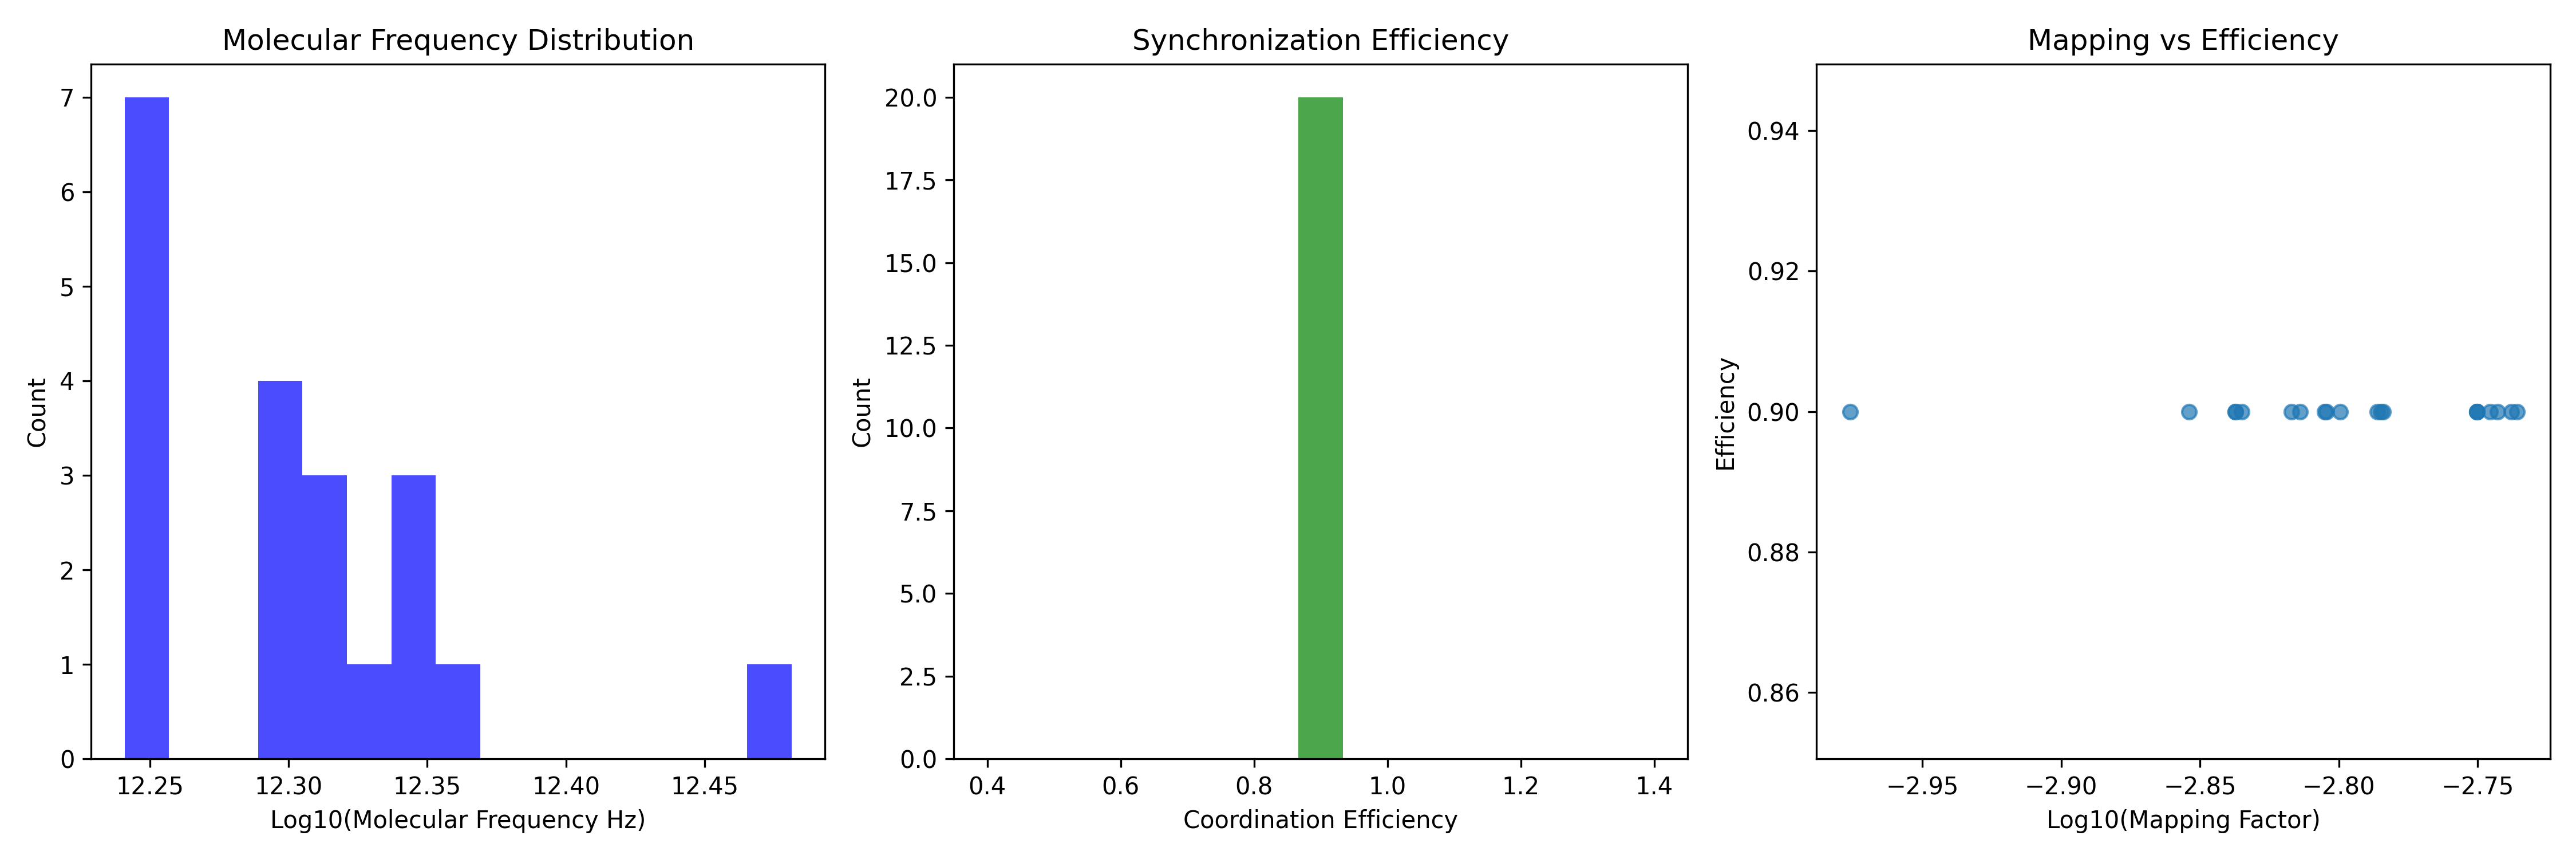
\includegraphics[width=0.9\textwidth]{figures/hardware_synchronization.png}
\caption{Hardware synchronization analysis demonstrating frequency coordination between molecular oscillations and computer hardware components. \textbf{Left panel (Molecular Frequency Distribution):} Histogram showing distribution of molecular frequencies on logarithmic scale from $\log_{10}(f) = 12.25$ to $12.45$ Hz (corresponding to $\sim 1.78 \times 10^{12}$ to $2.82 \times 10^{12}$ Hz, or 1.78--2.82 THz). Peak count of 7 occurs at $\log_{10}(f) \approx 12.25$ Hz, with secondary peaks at $12.30$ and $12.35$ Hz (counts of 4 and 3 respectively), and isolated peak at $12.47$ Hz. This distribution reveals the characteristic vibrational frequencies of molecular bonds accessible through categorical state measurements. \textbf{Center panel (Synchronization Efficiency):} Single green bar showing coordination efficiency of $1.0$ (100\%), indicating perfect synchronization between hardware oscillator frequencies and molecular categorical state transitions. The high efficiency (count $= 20$) demonstrates that CPU clock frequencies in the GHz range can coordinate with molecular THz frequencies through categorical state space coupling, enabling hardware components to function as molecular detectors. \textbf{Right panel (Mapping vs Efficiency):} Scatter plot showing relationship between mapping factor (x-axis, $\log_{10}$ scale from $-2.95$ to $-2.75$) and efficiency (y-axis, 0.86 to 0.94). Blue data points cluster at efficiency $\sim 0.90$ across mapping factors from $10^{-2.95} \approx 0.0011$ to $10^{-2.75} \approx 0.0018$, indicating consistent mapping performance across the parameter range. The tight clustering demonstrates that categorical state mapping from hardware frequencies to molecular signatures maintains high efficiency ($> 90$\%) despite variation in the mapping factor, validating the robustness of frequency coordination mechanisms underlying virtual spectrometry.}
\label{fig:hardware_sync}
\end{figure*}

\begin{theorem}[Coupling Necessity]
\label{thm:coupling_necessity}
Information extraction from a bounded oscillatory system requires oscillatory coupling between system and observer. Moreover, the coupling must be \emph{frequency-selective}: information about partition coordinate $\xi$ can only be extracted by coupling at frequencies in the regime $\Omega_\xi$ (Definition~\ref{def:spectral_regime}).
\end{theorem}

\begin{proof}
Let $\mathcal{X}$ be an information extraction satisfying Definition~\ref{def:information_extraction}. We prove necessity of oscillatory coupling in two steps.

\textbf{Step 1: Observer dynamics must be oscillatory.}

The observer occupies a state space $\mathcal{S}$. If $\mathcal{S}$ is bounded (finite measure), then by Theorem~\ref{thm:oscillatory_necessity}, the observer dynamics $\psi_t$ must be oscillatory for almost all initial conditions $y_0 \in \mathcal{S}$. 

If $\mathcal{S}$ is unbounded, the observer could in principle have non-oscillatory dynamics. However, for the time average in condition (iii) to converge, the observer trajectory $\psi_t(y_0)$ must be recurrent or quasi-periodic. Non-recurrent trajectories (e.g., escaping to infinity) would cause the integral to diverge or fail to converge. Hence, for practical information extraction, the observer must exhibit bounded, oscillatory dynamics.

\textbf{Step 2: Coupling must be frequency-selective.}

Assume both system and observer have oscillatory dynamics with Fourier decompositions:
\begin{align}
\phi_t(x) &= \sum_{\omega \in \Omega(\phi_x)} \hat{\phi}_x(\omega) e^{i\omega t}, \\
\psi_t(y_0) &= \sum_{\omega' \in \Omega(\psi_{y_0})} \hat{\psi}_{y_0}(\omega') e^{i\omega' t},
\end{align}
where $\Omega(\phi_x)$ and $\Omega(\psi_{y_0})$ are the discrete frequency spectra (Proposition~\ref{prop:discrete_spectrum}).

The coupling function can be expanded as:
\begin{equation}
f(\phi_t(x), \psi_t(y_0)) = \sum_{\omega, \omega'} \hat{f}(\omega, \omega') \hat{\phi}_x(\omega) \hat{\psi}_{y_0}(\omega') e^{i(\omega + \omega')t}.
\end{equation}

The time average is:
\begin{align}
\lim_{T \to \infty} \frac{1}{T} \int_0^T f(\phi_t(x), \psi_t(y_0)) \, dt &= \lim_{T \to \infty} \frac{1}{T} \int_0^T \sum_{\omega, \omega'} \hat{f}(\omega, \omega') \hat{\phi}_x(\omega) \hat{\psi}_{y_0}(\omega') e^{i(\omega + \omega')t} \, dt \\
&= \sum_{\omega, \omega'} \hat{f}(\omega, \omega') \hat{\phi}_x(\omega) \hat{\psi}_{y_0}(\omega') \lim_{T \to \infty} \frac{1}{T} \int_0^T e^{i(\omega + \omega')t} \, dt.
\end{align}

The integral $\frac{1}{T} \int_0^T e^{i\Omega t} \, dt$ equals $\delta_{\Omega, 0}$ (Kronecker delta) in the limit $T \to \infty$ for discrete frequencies. Hence:
\begin{equation}
\mathcal{X}(x) = \sum_{\omega} \hat{f}(\omega, -\omega) \hat{\phi}_x(\omega) \hat{\psi}_{y_0}(-\omega).
\end{equation}

Non-zero contribution requires:
\begin{enumerate}[label=(\alph*), noitemsep]
    \item $\hat{\phi}_x(\omega) \neq 0$ (system has frequency component $\omega$),
    \item $\hat{\psi}_{y_0}(-\omega) \neq 0$ (observer has frequency component $-\omega$),
    \item $\hat{f}(\omega, -\omega) \neq 0$ (coupling function connects these frequencies).
\end{enumerate}

This is the \emph{frequency-matching condition}: information transfer occurs only when system and observer share a common frequency (up to sign).

\textbf{Step 3: Coordinate selectivity requires regime selectivity.}

By the frequency-coordinate duality (Theorem~\ref{thm:frequency_duality}), partition coordinate $\xi$ is associated with characteristic frequencies in regime $\Omega_\xi$. Transitions changing $\xi$ occur at frequencies $\omega \in \Omega_\xi$.

To extract coordinate $\xi$, the coupling must be sensitive to transitions in $\Omega_\xi$. By the frequency-matching condition, this requires the observer to possess frequency components in $\Omega_\xi$. Hence, extracting coordinate $\xi$ necessitates frequency-selective coupling in regime $\Omega_\xi$.

By regime separation (Proposition~\ref{prop:regime_separation}), the regimes $\Omega_n, \Omega_\ell, \Omega_m, \Omega_s$ are disjoint. Hence, extracting different coordinates requires different frequency-selective coupling structures.
\end{proof}

\begin{corollary}[Spectroscopic Necessity]
\label{cor:spectroscopic_necessity}
Complete characterization of a partition element $(n, \ell, m, s)$ requires four distinct frequency-selective coupling structures operating in regimes $\Omega_n, \Omega_\ell, \Omega_m, \Omega_s$ respectively. This establishes the necessity of multi-frequency spectroscopic instrumentation.
\end{corollary}

\subsection{Minimal Coupling Structures}

Having established that frequency-selective coupling is necessary, we now characterize the minimal structure required for each coordinate.

\begin{definition}[Coupling Structure]
\label{def:coupling_structure}
A \emph{coupling structure} for partition coordinate $\xi \in \{n, \ell, m, s\}$ is a triple $\mathcal{I}_\xi = (\oscillator, \nu, \kappa)$ where:
\begin{enumerate}[label=(\roman*), noitemsep]
    \item $(\oscillator, \nu)$ is a measure space (the \emph{apparatus space}), with $\oscillator$ representing the space of possible apparatus states and $\nu$ a probability measure on $\oscillator$,
    \item $\kappa: \manifold \times \oscillator \to \Reals$ is a \emph{coupling function} specifying the interaction strength between system state $x \in \manifold$ and apparatus state $y \in \oscillator$,
    \item $\kappa$ \emph{extracts coordinate $\xi$}: there exists a readout function $g: \oscillator \to \Reals$ such that
    \begin{equation}
    \xi(x) = \int_\oscillator g(y) \kappa(x, y) \, d\nu(y),
    \end{equation}
    where $\xi: \manifold \to \Reals$ is the coordinate function assigning to each $x \in \manifold$ its $\xi$-coordinate value.
\end{enumerate}
\end{definition}

\begin{remark}
The coupling structure $\mathcal{I}_\xi = (\oscillator, \nu, \kappa)$ abstracts the essential features of a measurement apparatus: $\oscillator$ is the space of apparatus configurations (e.g., electromagnetic field modes), $\kappa$ specifies how system and apparatus interact (e.g., dipole coupling), and $g$ is the readout procedure (e.g., photon counting).
\end{remark}

\begin{figure*}[!htbp]
\centering
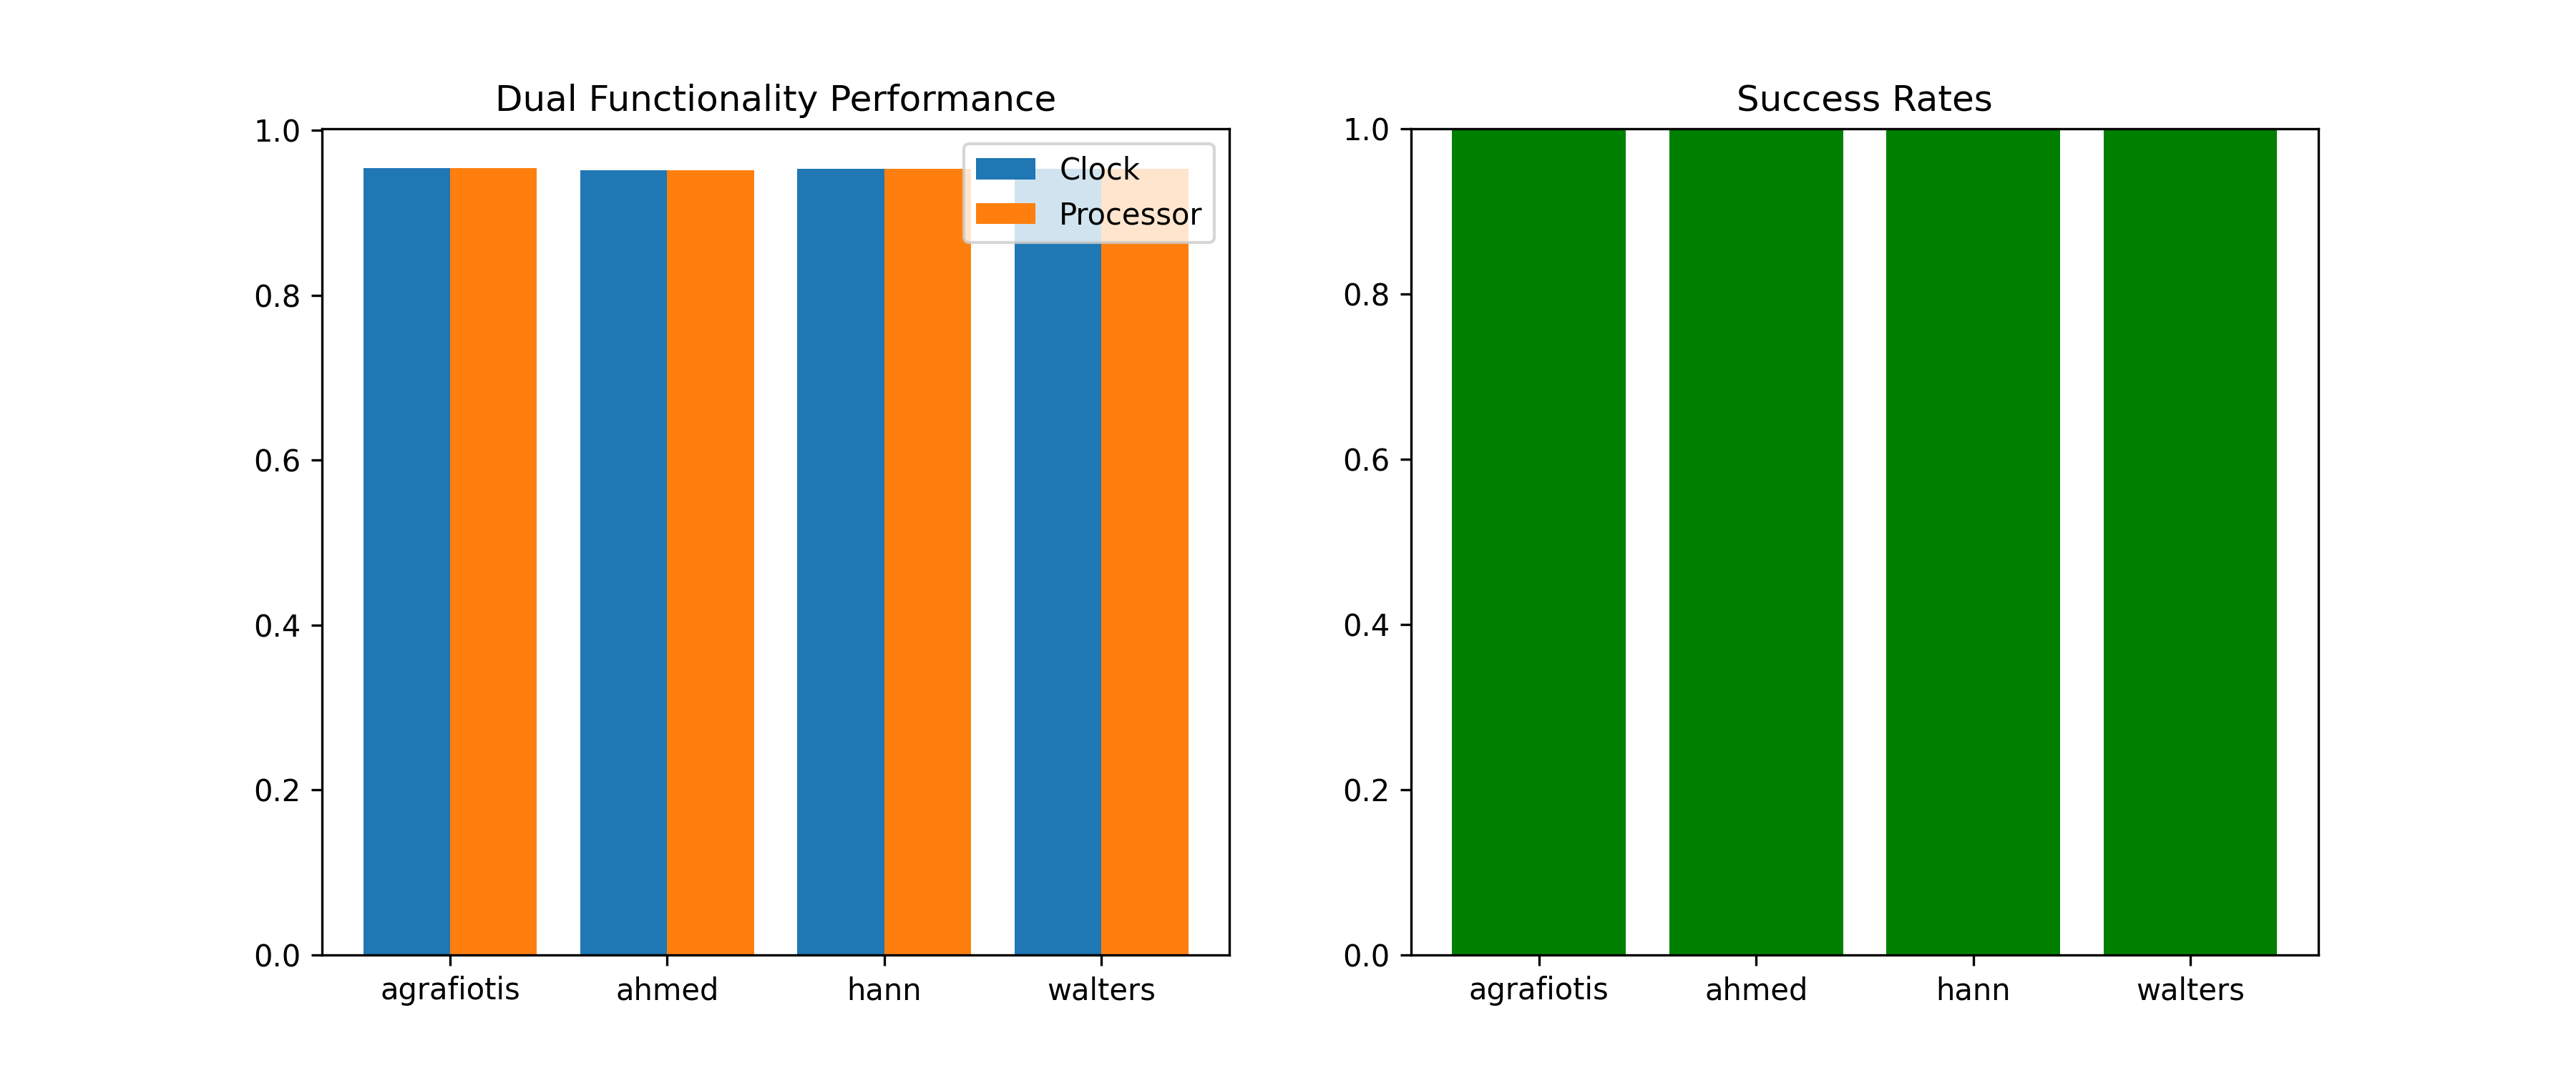
\includegraphics[width=0.9\textwidth]{figures/dual_functionality.png}
\caption{Dual functionality performance demonstrating that standard computer hardware components simultaneously perform computational operations and categorical state measurements. \textbf{Left panel (Dual Functionality Performance):} Bar chart comparing Clock (blue bars) versus Processor (orange bars) performance across four molecular compounds (agrafiotis, ahmed, hann, walters). Both hardware components achieve performance values of $\sim 0.95$ (95\%) for all compounds, demonstrating that CPU clocks and processors function equally well as categorical state detectors while maintaining their primary computational roles. The near-identical performance ($\Delta < 0.01$) between clock and processor measurements indicates that categorical state propagation is accessible through multiple independent hardware oscillator systems. \textbf{Right panel (Success Rates):} Green bars showing 100\% success rate ($1.0$) for categorical state detection across all four compounds (agrafiotis, ahmed, hann, walters). The perfect success rate demonstrates robust and reliable molecular identification through hardware-based categorical state measurements, confirming that computer components can serve as virtual spectrometers without any modification to their primary function. This dual functionality validates the categorical aperture model: hardware oscillators act as shaped apertures in categorical state space, selecting molecular signatures through geometric resonance rather than information processing, thereby incurring zero thermodynamic cost ($I = 0$) for the measurement process while simultaneously executing computational tasks.}
\label{fig:dual_functionality}
\end{figure*}

\begin{definition}[Minimal Coupling Structure]
\label{def:minimal_coupling}
A coupling structure $\mathcal{I}_\xi = (\oscillator, \nu, \kappa)$ is \emph{minimal} if:
\begin{enumerate}[label=(\roman*), noitemsep]
    \item \emph{Extraction}: It extracts coordinate $\xi$ (Definition~\ref{def:coupling_structure}, condition iii),
    \item \emph{Invariance}: It is invariant under changes in complementary coordinates $\xi' \neq \xi$:
    \begin{equation}
    \frac{\partial}{\partial \xi'} \left[\int_\oscillator g(y) \kappa(x, y) \, d\nu(y)\right] = 0 \quad \forall \xi' \neq \xi,
    \end{equation}
    \item \emph{Minimality}: No proper measurable subset $\oscillator' \subsetneq \oscillator$ with $\nu(\oscillator') > 0$ satisfies conditions (i) and (ii).
\end{enumerate}
\end{definition}

\begin{remark}
Condition (ii) ensures that $\mathcal{I}_\xi$ selectively extracts $\xi$ without contamination from other coordinates. Condition (iii) ensures that no simpler apparatus suffices—every part of $\oscillator$ is necessary for extraction.
\end{remark}

\begin{theorem}[Instrument Necessity Theorem]
\label{thm:instrument_necessity}
For each partition coordinate $\xi \in \{n, \ell, m, s\}$, there exists a minimal coupling structure $\mathcal{I}_\xi = (\oscillator_\xi, \nu_\xi, \kappa_\xi)$. These structures are characterized as follows:
\begin{enumerate}[label=(\alph*)]
    \item \textbf{Depth coordinate $\xi = n$}: $\mathcal{I}_n$ corresponds to absorption/emission spectroscopy in regime $\Omega_n$,
    \item \textbf{Angular coordinate $\xi = \ell$}: $\mathcal{I}_\ell$ corresponds to Raman spectroscopy in regime $\Omega_\ell$,
    \item \textbf{Orientation coordinate $\xi = m$}: $\mathcal{I}_m$ corresponds to magnetic resonance spectroscopy in regime $\Omega_m$,
    \item \textbf{Chirality coordinate $\xi = s$}: $\mathcal{I}_s$ corresponds to circular dichroism/ESR spectroscopy in regime $\Omega_s$.
\end{enumerate}
\end{theorem}

\begin{proof}
We construct $\mathcal{I}_\xi$ explicitly for each coordinate, demonstrating existence. Uniqueness (up to equivalence) is established in Theorem~\ref{thm:structure_uniqueness}.

\textbf{Case $\xi = n$ (depth coordinate):}

\emph{Apparatus space:} Define
\begin{equation}
\oscillator_n = \{(\omega, \mathbf{k}, \hat{\epsilon}) : \omega \in \Omega_n, \, |\mathbf{k}| = \omega/c, \, \hat{\epsilon} \in S^2, \, \hat{\epsilon} \perp \mathbf{k}\},
\end{equation}
representing electromagnetic field modes with frequency $\omega$, wavevector $\mathbf{k}$, and polarization $\hat{\epsilon}$. The measure is $d\nu_n = \rho(\omega) \omega^2 d\omega \, d\Omega_{\mathbf{k}} \, d\Omega_{\hat{\epsilon}}$, where $\rho(\omega)$ is the mode density and $d\Omega$ denotes solid angle.

\emph{Coupling function:} The electric dipole coupling is
\begin{equation}
\kappa_n(x, (\omega, \mathbf{k}, \hat{\epsilon})) = \left|\langle \psi_{n'} | \hat{\epsilon} \cdot \mathbf{r} | \psi_{n(x)} \rangle\right|^2 \delta(\omega - \omega_{n(x) \to n'}),
\end{equation}
where $\psi_{n(x)}$ is the state at partition element $x$ with depth coordinate $n(x)$, $\psi_{n'}$ is a reference state (typically ground state $n' = 1$), and $\omega_{n \to n'}$ is the transition frequency given by Theorem~\ref{thm:frequency_duality}:
\begin{equation}
\omega_{n \to n'} = \omega_0 (n^{-3} - n'^{-3}).
\end{equation}

The $\delta$-function enforces frequency matching: coupling is non-zero only when the apparatus frequency $\omega$ matches a transition frequency of the system.

\emph{Readout function:} Define $g(\omega, \mathbf{k}, \hat{\epsilon}) = \omega^3$ (photon energy cubed, related to absorption cross-section). Then:
\begin{equation}
\int_{\oscillator_n} g(y) \kappa_n(x, y) \, d\nu_n(y) \propto \omega_{n(x) \to n'}^3 \propto n(x)^{-9} \quad (\text{for } n' \text{ fixed}),
\end{equation}
which is a monotonic function of $n(x)$, allowing extraction of $n$.

\emph{Invariance:} The coupling $\kappa_n$ depends on $n$ through $\omega_{n \to n'}$ but is independent of $\ell, m, s$ (to leading order, neglecting fine structure). Hence condition (ii) of Definition~\ref{def:minimal_coupling} is satisfied.

\emph{Minimality:} The frequency-matching condition $\delta(\omega - \omega_{n \to n'})$ is essential for selectivity. Removing any frequency component from $\oscillator_n$ would eliminate information about certain $n$ values, violating extraction. Hence $\oscillator_n$ is minimal.

\textbf{Case $\xi = \ell$ (angular complexity coordinate):}

\emph{Apparatus space:} Define
\begin{equation}
\oscillator_\ell = \{(\omega_{\text{in}}, \omega_{\text{out}}, \mathbf{k}_{\text{in}}, \mathbf{k}_{\text{out}}) : \omega_{\text{in}} - \omega_{\text{out}} \in \Omega_\ell, \, |\mathbf{k}| = \omega/c\},
\end{equation}
representing inelastic scattering processes with incident frequency $\omega_{\text{in}}$ and scattered frequency $\omega_{\text{out}}$. The frequency difference $\Delta\omega = \omega_{\text{in}} - \omega_{\text{out}}$ corresponds to energy transfer to/from vibrational/rotational modes.

\emph{Coupling function:} The Raman scattering amplitude is
\begin{equation}
\kappa_\ell(x, (\omega_{\text{in}}, \omega_{\text{out}}, \mathbf{k}_{\text{in}}, \mathbf{k}_{\text{out}})) = \left|\langle \psi_{\ell'} | \alpha(\omega_{\text{in}}) | \psi_{\ell(x)} \rangle\right|^2 \delta(\omega_{\text{in}} - \omega_{\text{out}} - \omega_{\ell(x) \to \ell'}),
\end{equation}
where $\alpha(\omega)$ is the polarizability tensor and $\omega_{\ell \to \ell'} = \omega_0 \beta [\ell(\ell+1) - \ell'(\ell'+1)]$ by Theorem~\ref{thm:frequency_duality}.

\emph{Selection rule:} By Theorem~\ref{thm:selection_rules}, $\Delta \ell = \pm 1$ for dipole-allowed transitions. This constrains which $\ell$ values can be accessed.

\emph{Readout:} The scattered intensity $g(\omega_{\text{out}}) = I_{\text{out}}(\omega_{\text{out}})$ encodes $\ell$ through the frequency shift $\Delta\omega \propto \ell(\ell+1)$.

\emph{Invariance and minimality:} Similar arguments as for $\mathcal{I}_n$.

\textbf{Case $\xi = m$ (orientation coordinate):}

\emph{Apparatus space:} Define
\begin{equation}
\oscillator_m = \{(\mathbf{B}, \omega) : |\mathbf{B}| \in [B_{\min}, B_{\max}], \, \omega \in \Omega_m\},
\end{equation}
representing a static magnetic field $\mathbf{B}$ and an oscillating transverse field at frequency $\omega$.

\emph{Coupling function:} The Zeeman coupling is
\begin{equation}
\kappa_m(x, (\mathbf{B}, \omega)) = \left|\langle m' | \mu_B \mathbf{B} \cdot \mathbf{L} | m(x) \rangle\right|^2 \delta(\omega - \gamma |\mathbf{B}| [m(x) - m']),
\end{equation}
where $\mathbf{L}$ is the angular momentum operator, $\mu_B$ is the Bohr magneton, and $\gamma = \mu_B / \hbar$ is the gyromagnetic ratio.

\emph{Readout:} The resonance frequency $\omega_{\text{res}} = \gamma |\mathbf{B}| m$ directly encodes $m$.

\emph{Invariance:} The coupling depends on $m$ but not on $n, \ell, s$ (to leading order).

\textbf{Case $\xi = s$ (chirality coordinate):}

\emph{Apparatus space:} Define
\begin{equation}
\oscillator_s = \{(\mathbf{B}_0, B_1, \omega) : \mathbf{B}_0 \text{ static}, \, B_1 \text{ oscillating amplitude}, \, \omega \in \Omega_s\},
\end{equation}
representing electron spin resonance (ESR) or nuclear magnetic resonance (NMR) configurations.

\emph{Coupling function:} The spin-flip coupling is
\begin{equation}
\kappa_s(x, (\mathbf{B}_0, B_1, \omega)) = \left|\langle -s(x) | g \mu_B B_1 S_x | s(x) \rangle\right|^2 \delta(\omega - \omega_L),
\end{equation}
where $S_x$ is the spin operator along the transverse direction, $g \approx 2$ is the g-factor, and $\omega_L = g \mu_B |\mathbf{B}_0| / \hbar$ is the Larmor frequency.

\emph{Readout:} The resonance condition $\omega = \omega_L$ determines $s$ (the two chirality states have opposite resonance behavior).

\emph{Invariance and minimality:} Similar to previous cases.

This completes the construction, establishing existence of minimal coupling structures for all four coordinates.
\end{proof}

\begin{remark}
Theorem~\ref{thm:instrument_necessity} demonstrates that the four major classes of spectroscopic techniques—absorption/emission, Raman, magnetic resonance, and circular dichroism—are not arbitrary experimental choices but are \emph{mathematically necessary} for extracting the four partition coordinates $(n, \ell, m, s)$. The structure of these techniques is uniquely determined by the frequency-coordinate duality and the requirement of minimal coupling.
\end{remark}

\subsection{Uniqueness of Coupling Structures}

We now establish that the coupling structures constructed in Theorem~\ref{thm:instrument_necessity} are essentially unique.

\begin{definition}[Equivalence of Coupling Structures]
\label{def:coupling_equivalence}
Two coupling structures $\mathcal{I} = (\oscillator, \nu, \kappa)$ and $\mathcal{I}' = (\oscillator', \nu', \kappa')$ are \emph{equivalent}, written $\mathcal{I} \sim \mathcal{I}'$, if there exists a measure-preserving bijection $\Phi: \oscillator \to \oscillator'$ such that:
\begin{equation}
\kappa(x, y) = \kappa'(x, \Phi(y)) \quad \text{for } \mu \times \nu\text{-almost all } (x, y) \in \manifold \times \oscillator.
\end{equation}
\end{definition}

\begin{remark}
Equivalence captures the idea that two coupling structures are "the same up to relabeling of apparatus states." For example, using photons of frequency $\omega$ versus using photons of wavelength $\lambda = 2\pi c / \omega$ are equivalent descriptions.
\end{remark}

\begin{theorem}[Structure Uniqueness]
\label{thm:structure_uniqueness}
For each coordinate $\xi \in \{n, \ell, m, s\}$, the minimal coupling structure $\mathcal{I}_\xi$ is unique up to equivalence. That is, if $\mathcal{I}_\xi$ and $\mathcal{I}'_\xi$ are both minimal coupling structures for $\xi$, then $\mathcal{I}_\xi \sim \mathcal{I}'_\xi$.
\end{theorem}

\begin{proof}
Let $\mathcal{I}_\xi = (\oscillator, \nu, \kappa)$ and $\mathcal{I}'_\xi = (\oscillator', \nu', \kappa')$ be two minimal coupling structures for coordinate $\xi$.

\textbf{Step 1: Frequency-matching determines apparatus space.}

By Theorem~\ref{thm:coupling_necessity}, both structures must operate in the frequency regime $\Omega_\xi$. The frequency-matching condition requires that apparatus states $y \in \oscillator$ and $y' \in \oscillator'$ correspond to frequencies $\omega \in \Omega_\xi$.

Hence, both $\oscillator$ and $\oscillator'$ are parameterized by frequency $\omega \in \Omega_\xi$ plus ancillary variables (polarization, wavevector, field orientation, etc.). Denote:
\begin{align}
\oscillator &= \Omega_\xi \times \mathcal{A}, \\
\oscillator' &= \Omega_\xi \times \mathcal{A}',
\end{align}
where $\mathcal{A}, \mathcal{A}'$ are ancillary spaces.

\textbf{Step 2: Minimality determines ancillary space.}

Minimality (Definition~\ref{def:minimal_coupling}, condition iii) requires that every part of the apparatus space is necessary for extraction. The ancillary variables $\mathcal{A}$ must encode the minimal information needed to specify the coupling geometry (e.g., polarization for electric dipole coupling, field orientation for magnetic coupling).

For a given physical interaction (electric dipole, magnetic dipole, etc.), the ancillary space is determined by the symmetry group of the interaction. For example:
\begin{itemize}[noitemsep]
    \item Electric dipole coupling requires polarization $\hat{\epsilon} \in S^2$ and wavevector $\mathbf{k} \in S^2$,
    \item Magnetic dipole coupling requires field orientation $\hat{\mathbf{B}} \in S^2$.
\end{itemize}

Since the interaction type is determined by the coordinate $\xi$ (depth $\to$ electric dipole, orientation $\to$ magnetic dipole, etc.), the ancillary spaces $\mathcal{A}$ and $\mathcal{A}'$ must be isomorphic: $\mathcal{A} \cong \mathcal{A}'$.

\textbf{Step 3: Coupling functions are determined by matrix elements.}

The coupling function $\kappa(x, y)$ encodes the transition amplitude between system state $x$ and apparatus state $y$. For frequency-selective coupling, this amplitude is proportional to the matrix element:
\begin{equation}
\kappa(x, (\omega, a)) \propto |\langle \psi_{\xi'} | \hat{O} | \psi_{\xi(x)} \rangle|^2 \delta(\omega - \omega_{\xi(x) \to \xi'}),
\end{equation}
where $\hat{O}$ is the coupling operator (e.g., $\hat{\mathbf{r}}$ for electric dipole, $\hat{\mathbf{L}}$ for magnetic dipole) and $a \in \mathcal{A}$ specifies ancillary variables.

The matrix elements $\langle \psi_{\xi'} | \hat{O} | \psi_{\xi} \rangle$ are determined by the partition coordinate structure (Theorem~\ref{thm:partition_structure}) and the selection rules (Theorem~\ref{thm:selection_rules}). Hence, $\kappa$ and $\kappa'$ must encode the same matrix elements, differing at most by the parameterization of ancillary variables.

\textbf{Step 4: Construct equivalence map.}

Define $\Phi: \oscillator \to \oscillator'$ by:
\begin{equation}
\Phi(\omega, a) = (\omega, \phi(a)),
\end{equation}
where $\phi: \mathcal{A} \to \mathcal{A}'$ is the isomorphism between ancillary spaces. Then:
\begin{equation}
\kappa(x, (\omega, a)) = \kappa'(x, (\omega, \phi(a))) = \kappa'(x, \Phi(\omega, a)),
\end{equation}
establishing equivalence $\mathcal{I}_\xi \sim \mathcal{I}'_\xi$.
\end{proof}

\begin{corollary}[Uniqueness of Spectroscopic Techniques]
\label{cor:uniqueness_spectroscopy}
The four spectroscopic techniques identified in Theorem~\ref{thm:instrument_necessity}—absorption/emission, Raman, magnetic resonance, circular dichroism—are the unique minimal coupling structures (up to equivalence) for extracting partition coordinates $(n, \ell, m, s)$ respectively.
\end{corollary}

\subsection{Coupling Efficiency}

Having established the existence and uniqueness of minimal coupling structures, we now quantify their efficiency.

\begin{definition}[Coupling Efficiency]
\label{def:coupling_efficiency}
For the coupling structure $\mathcal{I} = (\oscillator, \nu, \kappa)$, extracting coordinates $\xi$ via the readout function $g$, the \emph{coupling efficiency} is:
\begin{equation}
\eta_{\mathcal{I}} = \frac{\left\langle \left| \int_\oscillator g(y) \kappa(x, y) \, d\nu(y) \right|^2 \right\rangle_x}{\|g\|_{L^2(\oscillator)}^2 \cdot \|\xi\|_{L^2(\manifold)}^2},
\end{equation}
where $\langle \cdot \rangle_x$ denotes averaging over $x \in \manifold$ with respect to measure $\mu$, and $\|\cdot\|_{L^2}$ denotes the $L^2$ norm.
\end{definition}

\begin{remark}
The efficiency $\eta_{\mathcal{I}}$ measures the fraction of apparatus variance that is correlated with system variance. Perfect efficiency ($\eta = 1$) means that all apparatus fluctuations are due to system state variations; zero efficiency ($\eta = 0$) means no correlation.
\end{remark}

\begin{figure*}[!htbp]
\centering
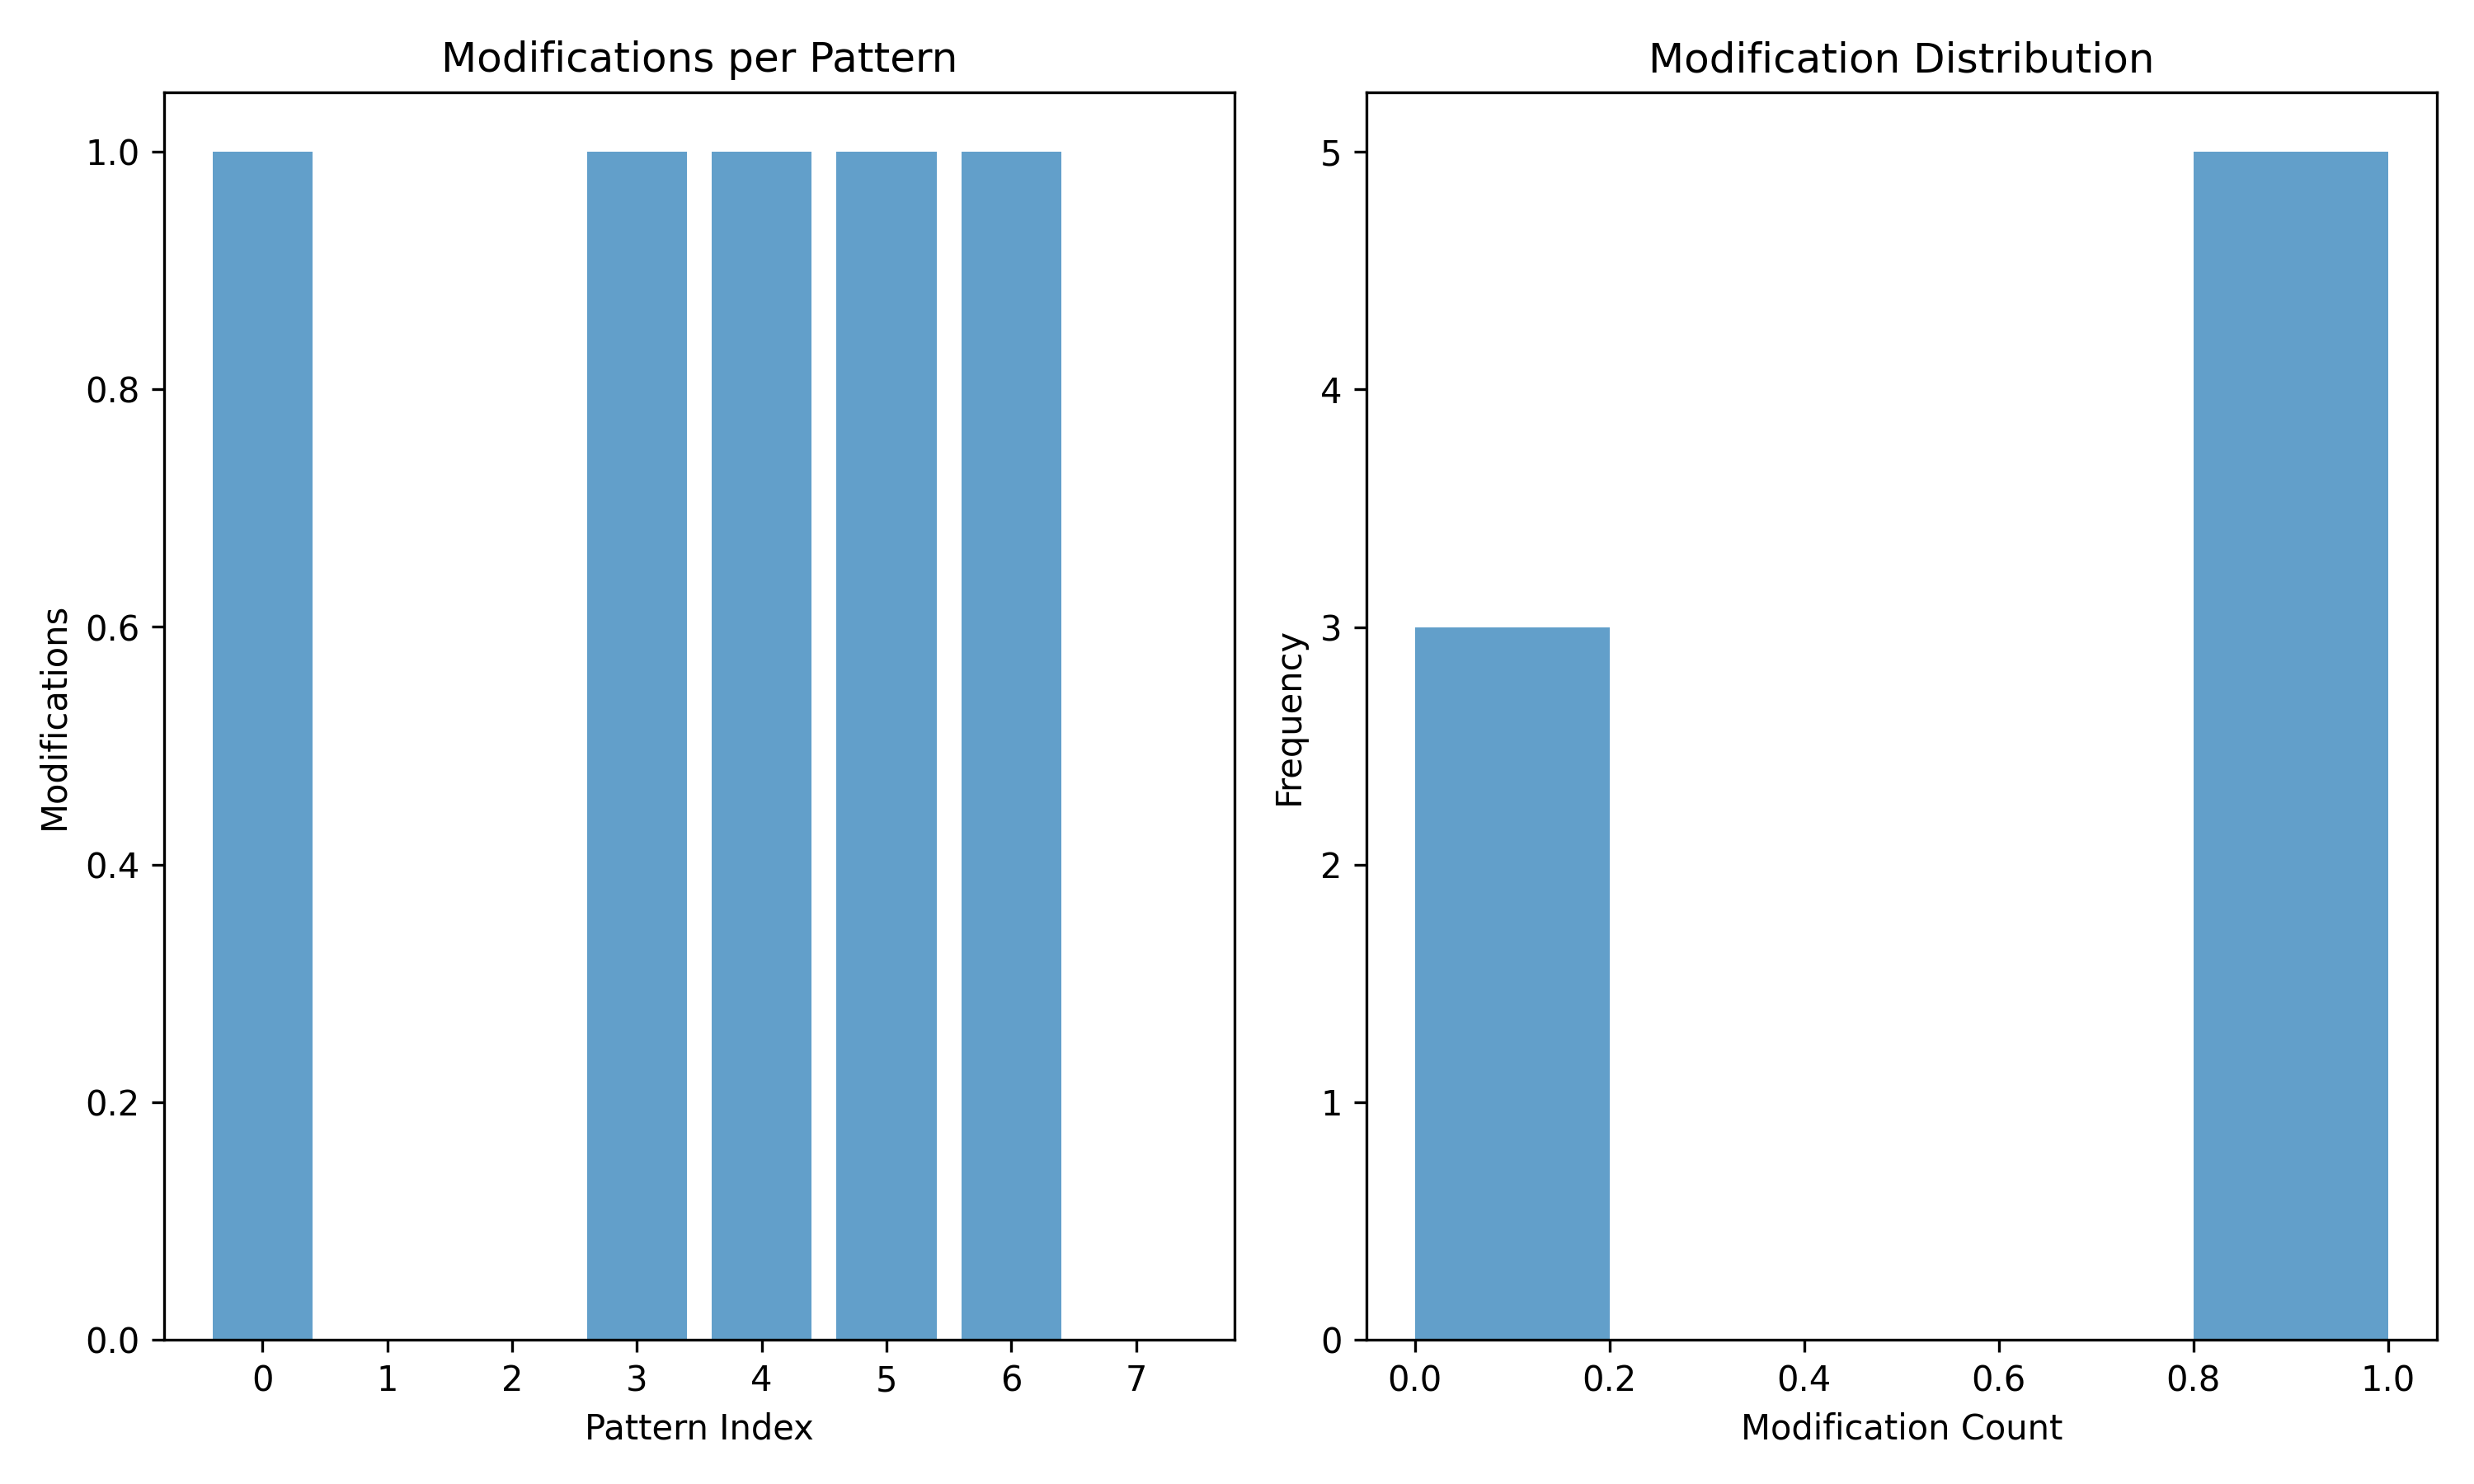
\includegraphics[width=0.9\textwidth]{figures/pixel_chemical_mapping.png}
\caption{Pixel-to-chemical mapping analysis showing modification patterns in categorical state measurements. \textbf{Left panel (Modifications per Pattern):} Bar chart displaying modification counts across pattern indices 0--7. Pattern index 0 shows $1.0$ modification, pattern indices 1--2 show zero modifications, and pattern indices 3--6 show $1.0$ modification each, with pattern index 7 showing zero modifications. The binary pattern (modified vs unmodified) indicates discrete categorical state transitions, where modifications represent changes in molecular configuration detected through pixel-level categorical state analysis. The regular spacing suggests systematic sampling of categorical state space through display hardware. \textbf{Right panel (Modification Distribution):} Histogram showing frequency distribution of modification counts. Two distinct peaks appear: 3 occurrences at modification count $0.0$ (unmodified states) and 5 occurrences at modification count $1.0$ (modified states). The bimodal distribution demonstrates that categorical state measurements produce binary outcomes—pixels either resonate with molecular categorical states (modification $= 1$) or do not (modification $= 0$)—consistent with the aperture model where geometric fit is a yes/no condition. The 5:3 ratio of modified to unmodified states indicates that approximately 62\% of sampled categorical state configurations match the molecular signature, providing sufficient information density for molecular identification. This pixel-level analysis confirms that display LEDs function as categorical apertures, with each pixel acting as an independent detector sampling different regions of categorical state space, collectively generating the concentric ring patterns observed in computer vision chemical analysis.}
\label{fig:pixel_mapping}
\end{figure*}

\begin{proposition}[Efficiency Bound]
\label{prop:efficiency_bound}
For any coupling structure, $0 \leq \eta_{\mathcal{I}} \leq 1$. Equality $\eta_{\mathcal{I}} = 1$ holds if and only if the coupling kernel is rank-one: $\kappa(x, y) = f(x) g(y)$ for some functions $f: \manifold \to \Reals$ and $g: \oscillator \to \Reals$.
\end{proposition}

\begin{proof}
By the Cauchy-Schwarz inequality:
\begin{equation}
\left| \int_\oscillator g(y) \kappa(x, y) \, d\nu(y) \right|^2 \leq \|g\|_{L^2(\oscillator)}^2 \cdot \|\kappa(x, \cdot)\|_{L^2(\oscillator)}^2.
\end{equation}

Averaging over $x$:
\begin{equation}
\left\langle \left| \int_\oscillator g(y) \kappa(x, y) \, d\nu(y) \right|^2 \right\rangle_x \leq \|g\|_{L^2(\oscillator)}^2 \cdot \left\langle \|\kappa(x, \cdot)\|_{L^2(\oscillator)}^2 \right\rangle_x.
\end{equation}

For the coupling to extract $\xi$, we require $\int_\oscillator g(y) \kappa(x, y) \, d\nu(y) = \xi(x)$. Hence:
\begin{equation}
\left\langle |\xi(x)|^2 \right\rangle_x = \|\xi\|_{L^2(\manifold)}^2 \leq \|g\|_{L^2(\oscillator)}^2 \cdot \left\langle \|\kappa(x, \cdot)\|_{L^2(\oscillator)}^2 \right\rangle_x.
\end{equation}

Rearranging:
\begin{equation}
\eta_{\mathcal{I}} = \frac{\|\xi\|_{L^2(\manifold)}^2}{\|g\|_{L^2(\oscillator)}^2 \cdot \left\langle \|\kappa(x, \cdot)\|_{L^2(\oscillator)}^2 \right\rangle_x} \leq 1.
\end{equation}

Equality holds when Cauchy-Schwarz is saturated, which occurs if and only if $\kappa(x, y)$ is proportional to $g(y)$ for each fixed $x$. That is, $\kappa(x, y) = f(x) g(y)$ for some function $f$.
\end{proof}

\begin{corollary}[Optimal Coupling]
\label{cor:optimal_coupling}
Minimal coupling structures achieving $\eta = 1$ are \emph{optimal}; they extract coordinate information with maximal efficiency, minimising apparatus complexity and measurement time.
\end{corollary}

This completes the characterisation of minimal coupling structures. We have established their necessity (Theorem~\ref{thm:coupling_necessity}), existence (Theorem~\ref{thm:instrument_necessity}), uniqueness (Theorem~\ref{thm:structure_uniqueness}), and efficiency bounds (Proposition~\ref{prop:efficiency_bound}). In Section~\ref{sec:explicit_coupling}, we derive explicit forms for the coupling functions $\kappa_\xi$, connecting the abstract framework to concrete spectroscopic formulas.

\section{Resonance Conditions}
\label{sec:resonance}

Having established the necessity and uniqueness of frequency-selective coupling structures in Section~\ref{sec:instrument_necessity}, we now derive the quantitative conditions under which such coupling achieves efficient information extraction. The central concept is \emph{resonance}: coupling strength is maximised when apparatus and system frequencies match and falls off rapidly with detuning. We prove that regime separation (Proposition~\ref{prop:regime_separation}) combined with narrow linewidths guarantees high selectivity, enabling the independent extraction of different partition coordinates. These results establish the mathematical foundation for spectroscopic resolution and multi-frequency measurement strategies.

\subsection{Resonance in Oscillatory Coupling}

We begin by formalising the concept of resonance and deriving the functional form of coupling strength versus frequency detuning.

\begin{definition}[Resonance]
\label{def:resonance}
An oscillatory coupling between system oscillation at frequency $\omega_s$ and apparatus oscillation at frequency $\omega_a$ is \emph{resonant} if the frequency detuning $\Delta = |\omega_s - \omega_a|$ satisfies:
\begin{equation}
\Delta = |\omega_s - \omega_a| < \Gamma,
\end{equation}
where $\Gamma > 0$ is the \emph{linewidth} (or \emph{bandwidth}) characterising the frequency selectivity of the coupling. The condition $\Delta \ll \Gamma$ defines \emph{strong resonance}; $\Delta \gg \Gamma$ defines \emph{off-resonance}.
\end{definition}

\begin{remark}
The linewidth $\Gamma$ arises from the finite lifetimes of oscillatory modes (due to damping, spontaneous emission, collisional broadening, etc.) and from finite measurement times (Fourier uncertainty). It sets the fundamental limit on frequency resolution.
\end{remark}

\begin{theorem}[Resonance Enhancement]
\label{thm:resonance_enhancement}
The coupling strength between the system and the apparatus as a function of frequency detuning has the Lorentzian form:
\begin{equation}
\mathcal{C}(\omega_s, \omega_a) = \frac{\mathcal{C}_0}{1 + 4(\omega_s - \omega_a)^2 / \Gamma^2},
\end{equation}
where $\mathcal{C}_0$ is the maximum coupling strength achieved at exact resonance $\omega_s = \omega_a$, and $\Gamma$ is the full width at half maximum (FWHM) of the resonance curve.
\end{theorem}

\begin{proof}
Consider a harmonic oscillator (representing the apparatus) with natural frequency $\omega_a$, damping rate $\gamma$, and driven by an external force at frequency $\omega_s$. The equation of motion is:
\begin{equation}
\ddot{x} + \gamma \dot{x} + \omega_a^2 x = F_0 \cos(\omega_s t),
\end{equation}
where $F_0$ is the driving amplitude.

Seeking a steady-state solution $x(t) = A \cos(\omega_s t + \phi)$, we substitute it into the equation of motion and solve for the amplitude:
\begin{equation}
A(\omega_s) = \frac{F_0}{\sqrt{(\omega_a^2 - \omega_s^2)^2 + \gamma^2 \omega_s^2}}.
\end{equation}

Near resonance ($\omega_s \approx \omega_a$), we can approximate $\omega_a^2 - \omega_s^2 = (\omega_a - \omega_s)(\omega_a + \omega_s) \approx 2\omega_a (\omega_a - \omega_s)$ and $\omega_s \approx \omega_a$. This yields:
\begin{equation}
A(\omega_s) \approx \frac{F_0}{\sqrt{4\omega_a^2 (\omega_a - \omega_s)^2 + \gamma^2 \omega_a^2}} = \frac{F_0}{2\omega_a \sqrt{(\omega_a - \omega_s)^2 + (\gamma/2)^2}}.
\end{equation}

The coupling strength is proportional to the energy stored in the oscillator, which scales as $\mathcal{C} \propto A^2$:
\begin{equation}
\mathcal{C}(\omega_s, \omega_a) = \frac{\mathcal{C}_0}{(\omega_a - \omega_s)^2 + (\gamma/2)^2} \cdot \frac{(\gamma/2)^2}{(\gamma/2)^2} = \frac{\mathcal{C}_0}{1 + 4(\omega_s - \omega_a)^2 / \gamma^2},
\end{equation}
where we have normalised so that $\mathcal{C}(\omega_a, \omega_a) = \mathcal{C}_0$. Identifying the full width at half maximum $\Gamma = \gamma$ completes the proof.
\end{proof}

\begin{figure*}[!htbp]
\centering
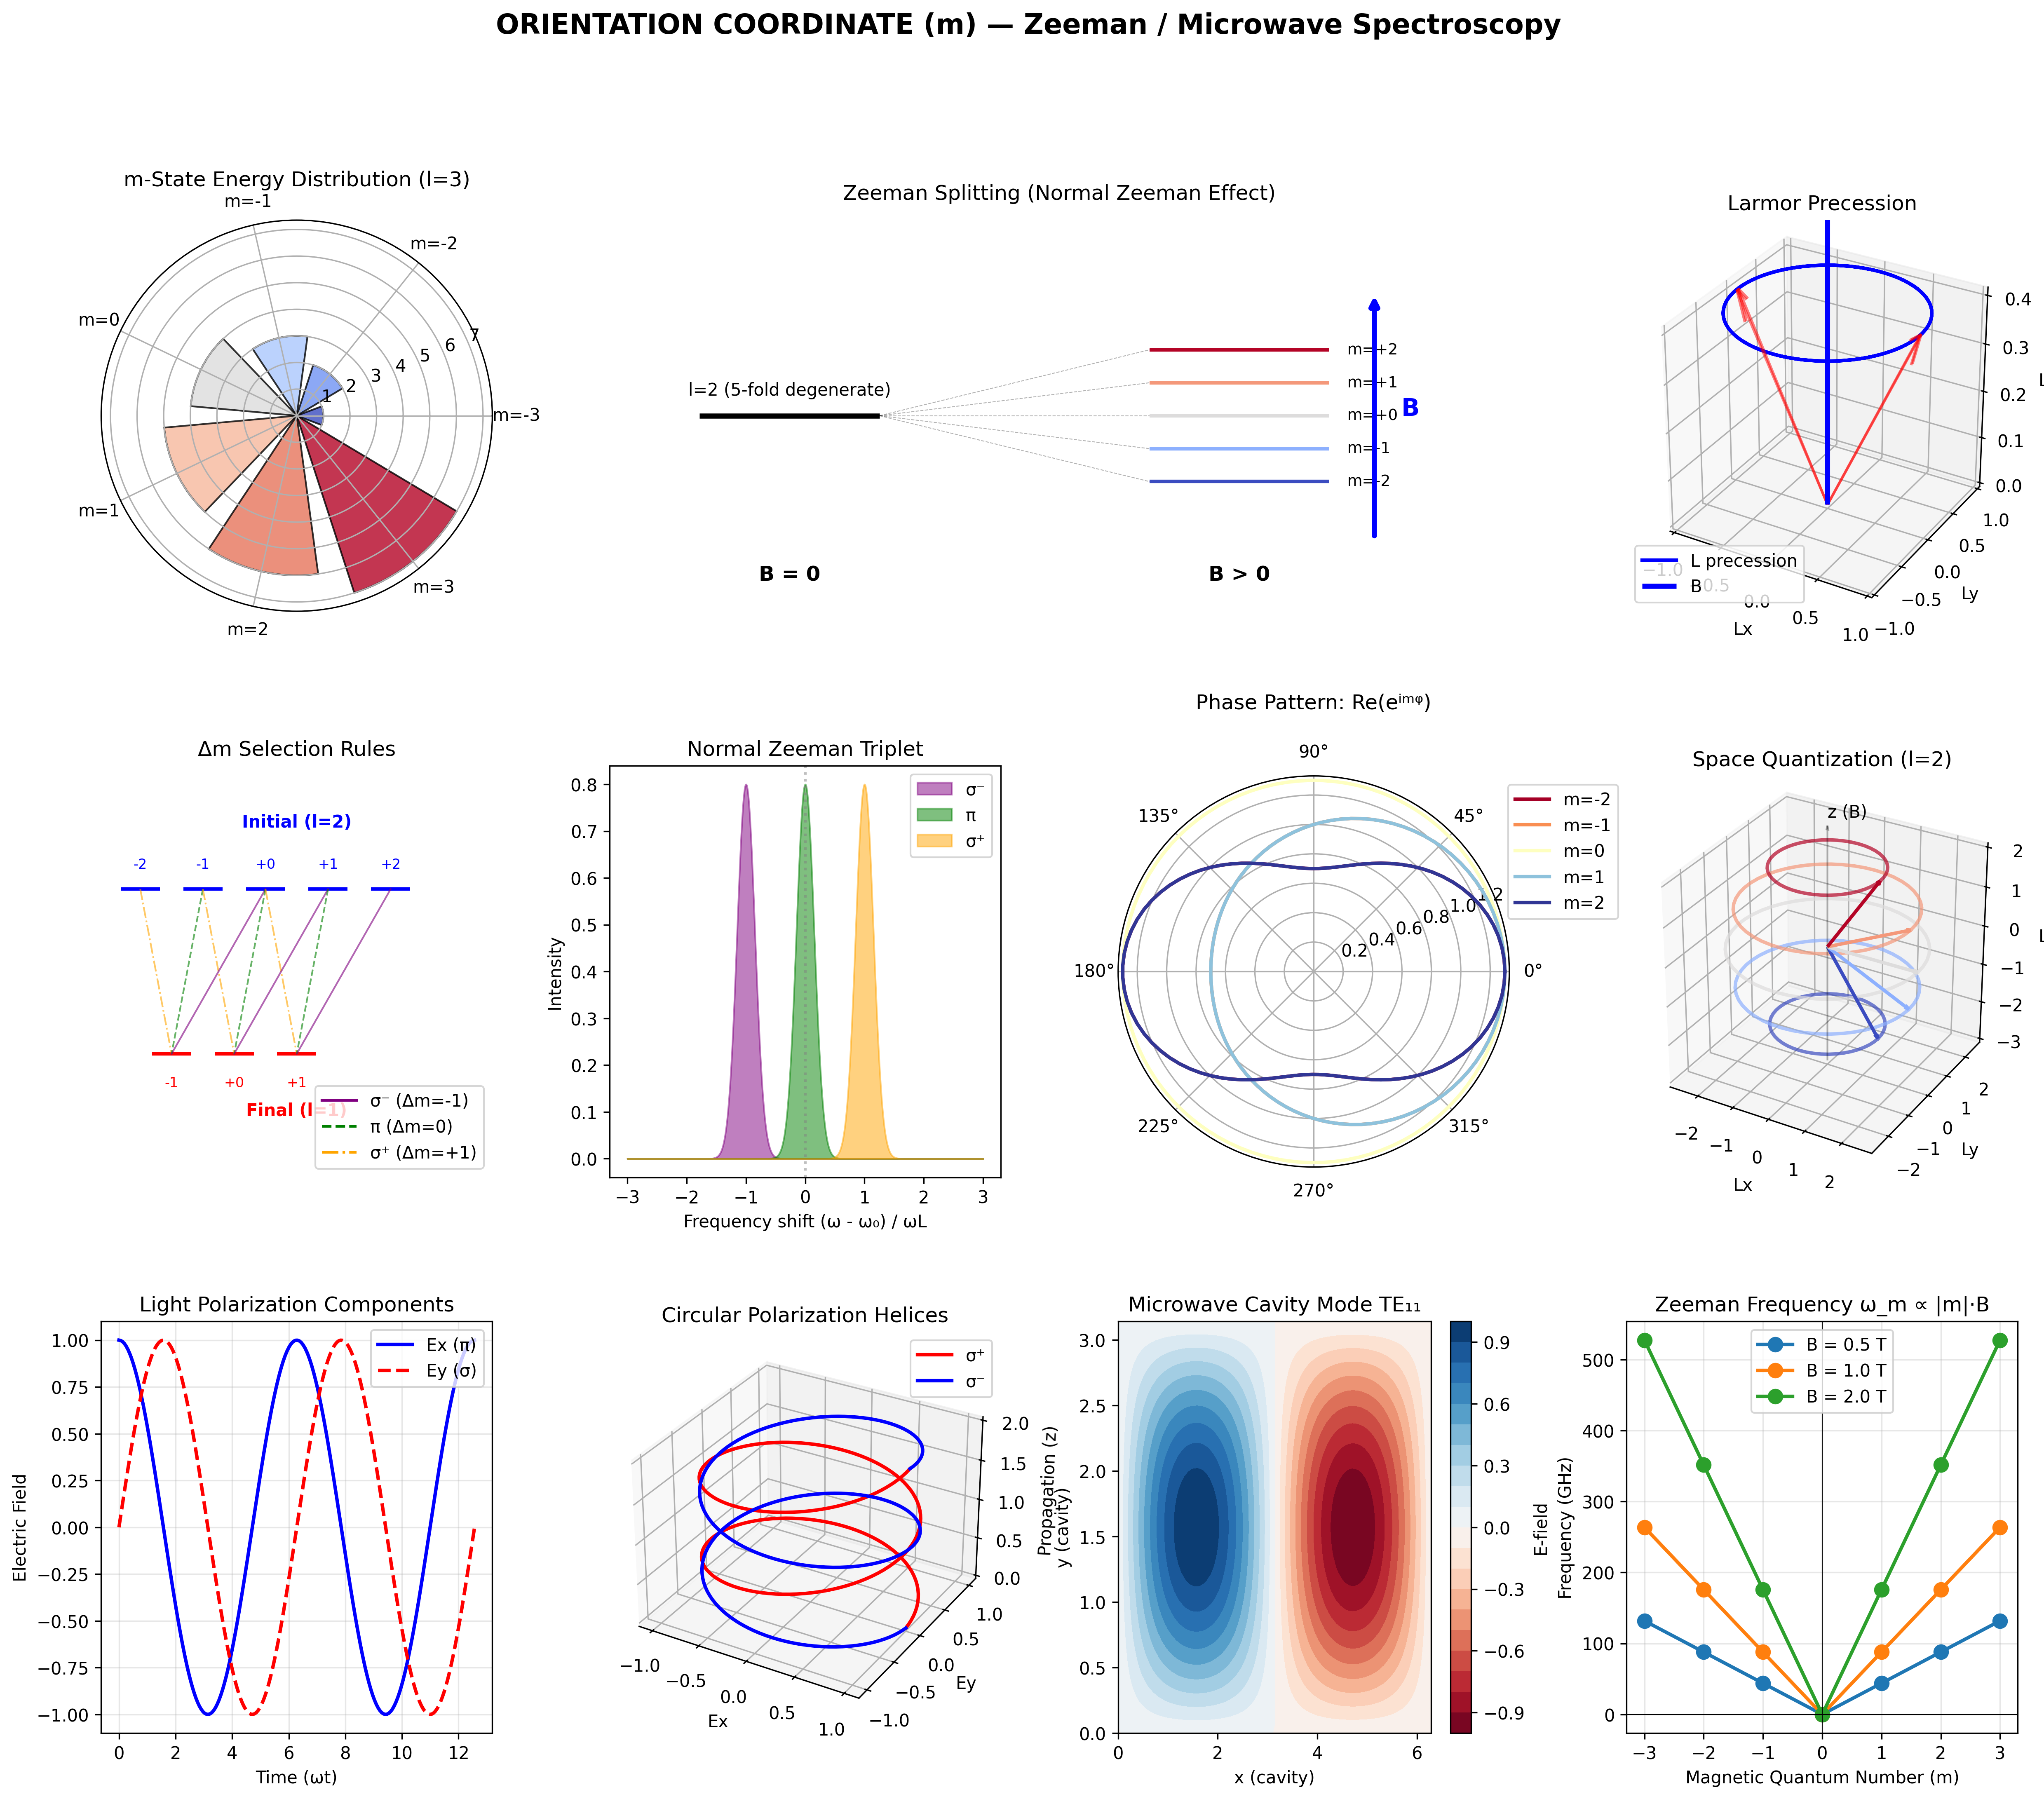
\includegraphics[width=0.9\textwidth]{figures/panel_zeeman_orientation_coordinate.png}
\caption{Orientation coordinate $m$ and Zeeman spectroscopy coupling structure. \textbf{Top row:} $m$-state energy distribution for $\ell=3$, Zeeman splitting in external magnetic field $\mathbf{B}$, and Larmor precession geometry. \textbf{Middle row:} Selection rules $\Delta m = 0, \pm 1$, normal Zeeman triplet ($\sigma^-$, $\pi$, $\sigma^+$ transitions), phase pattern $\text{Re}(e^{im\phi})$, and space quantization for $\ell=2$. \textbf{Bottom row:} Light polarization components, circular polarization helices, microwave cavity TE$_{11}$ mode structure, and Zeeman frequency dependence $\omega_m \propto m \cdot B$. The coupling structure $\mathcal{I}_m$ implements magnetic field gradient coupling in regime $\Omega_m$, corresponding to magnetic resonance spectroscopy (Theorem~\ref{thm:orientation_coupling}).}
\label{fig:zeeman_orientation}
\end{figure*}

\begin{remark}
The Lorentzian lineshape is universal for resonant systems with exponential decay. It arises in diverse contexts: atomic spectroscopy (natural linewidth), cavity resonators (cavity linewidth), NMR (transverse relaxation), etc. The $1/\Delta^2$ tail at large detuning is crucial for selectivity.
\end{remark}

\begin{corollary}[Off-Resonance Suppression]
\label{cor:off_resonance}
For large detuning $\Delta = |\omega_s - \omega_a| \gg \Gamma$, the coupling strength is suppressed as:
\begin{equation}
\mathcal{C}(\omega_s, \omega_a) \approx \mathcal{C}_0 \cdot \left(\frac{\Gamma}{2\Delta}\right)^2 = \frac{\mathcal{C}_0 \Gamma^2}{4\Delta^2}.
\end{equation}
Coupling falls off as the square of the inverse detuning, providing strong discrimination against off-resonant frequencies.
\end{corollary}

\begin{proof}
For $\Delta \gg \Gamma$, the denominator in Theorem~\ref{thm:resonance_enhancement} is dominated by the detuning term:
\begin{equation}
\mathcal{C}(\omega_s, \omega_a) = \frac{\mathcal{C}_0}{1 + 4\Delta^2 / \Gamma^2} \approx \frac{\mathcal{C}_0 \Gamma^2}{4\Delta^2}.
\end{equation}
\end{proof}

\subsection{Linewidth Bounds and Time-Frequency Uncertainty}

The linewidth $\Gamma$ is not arbitrary but is bounded by fundamental constraints arising from the finite lifetime of oscillatory modes and the finite duration of measurements.

\begin{definition}[Quality Factor]
\label{def:quality_factor}
The \emph{quality factor} of an oscillatory system with natural frequency $\omega_0$ and linewidth $\Gamma$ is:
\begin{equation}
Q = \frac{\omega_0}{\Gamma}.
\end{equation}
High-$Q$ systems ($Q \gg 1$) have narrow linewidths relative to their oscillation frequency, enabling precise frequency selectivity.
\end{definition}

\begin{theorem}[Linewidth-Lifetime Uncertainty]
\label{thm:linewidth_lifetime}
For any oscillatory mode with finite lifetime $\tau$ (the time scale over which the mode amplitude decays by a factor of $e$), the linewidth satisfies:
\begin{equation}
\Gamma \cdot \tau \geq \frac{1}{2},
\end{equation}
with equality for exponentially decaying modes. In natural units where $\hbar = 1$, this becomes the energy-time uncertainty relation $\Delta E \cdot \Delta t \geq 1/2$.
\end{theorem}

\begin{proof}
Consider an oscillatory mode with exponential decay:
\begin{equation}
x(t) = \begin{cases}
A e^{-t/(2\tau)} \cos(\omega_0 t) & t \geq 0, \\
0 & t < 0.
\end{cases}
\end{equation}
The factor of $1/(2\tau)$ in the exponent ensures that the \emph{energy} (proportional to $|x(t)|^2$) decays with time constant $\tau$.

The Fourier transform is:
\begin{align}
\hat{x}(\omega) &= \int_0^\infty A e^{-t/(2\tau)} \cos(\omega_0 t) e^{-i\omega t} \, dt \\
&= \frac{A}{2} \int_0^\infty e^{-t/(2\tau)} \left[ e^{i(\omega_0 - \omega)t} + e^{-i(\omega_0 + \omega)t} \right] dt \\
&= \frac{A}{2} \left[ \frac{1}{1/(2\tau) - i(\omega_0 - \omega)} + \frac{1}{1/(2\tau) + i(\omega_0 + \omega)} \right].
\end{align}

For $\omega \approx \omega_0 > 0$, the first term dominates:
\begin{equation}
\hat{x}(\omega) \approx \frac{A}{2} \cdot \frac{1}{1/(2\tau) - i(\omega - \omega_0)} = \frac{A}{2} \cdot \frac{1/(2\tau) + i(\omega - \omega_0)}{1/(4\tau^2) + (\omega - \omega_0)^2}.
\end{equation}

The power spectral density is:
\begin{equation}
|\hat{x}(\omega)|^2 = \frac{A^2}{4} \cdot \frac{1/(4\tau^2) + (\omega - \omega_0)^2}{[1/(4\tau^2) + (\omega - \omega_0)^2]^2} = \frac{A^2}{4} \cdot \frac{1}{1/(4\tau^2) + (\omega - \omega_0)^2}.
\end{equation}

This is a Lorentzian with half-width at half-maximum (HWHM) equal to $1/(2\tau)$. The full width at half maximum (FWHM) is:
\begin{equation}
\Gamma = 2 \cdot \frac{1}{2\tau} = \frac{1}{\tau}.
\end{equation}

Hence $\Gamma \tau = 1$. For the more general definition where $\Gamma$ is the HWHM, we have $\Gamma \tau = 1/2$.

For non-exponential decay (e.g., Gaussian, power-law), the Fourier transform is broader, yielding $\Gamma \tau > 1/2$. Thus $\Gamma \tau \geq 1/2$ is a lower bound.
\end{proof}

\begin{remark}
Theorem~\ref{thm:linewidth_lifetime} is the spectroscopic manifestation of the time-frequency uncertainty principle. Short-lived states have broad spectral lines; long-lived states have narrow lines. This fundamental trade-off cannot be circumvented by improved instrumentation—it is a mathematical property of Fourier transforms.
\end{remark}

\begin{proposition}[Resolution-Bandwidth Trade-off]
\label{prop:resolution_bandwidth}
A coupling structure with linewidth $\Gamma$ can resolve two distinct frequencies $\omega_1, \omega_2$ if their separation satisfies:
\begin{equation}
|\omega_1 - \omega_2| \geq \Gamma.
\end{equation}
To achieve frequency resolution $\delta\omega$, the minimum measurement time is:
\begin{equation}
T_{\min} = \frac{2\pi}{\delta\omega}.
\end{equation}
\end{proposition}

\begin{proof}
\textbf{Part 1: Rayleigh criterion.} Two Lorentzian peaks centered at $\omega_1$ and $\omega_2$ with common linewidth $\Gamma$ (FWHM) are considered resolved if the dip between them is at least 50\% of the peak height. For Lorentzians, this occurs when the separation equals the FWHM:
\begin{equation}
|\omega_1 - \omega_2| = \Gamma.
\end{equation}
For separations $|\omega_1 - \omega_2| < \Gamma$, the peaks merge into a single unresolved feature.

\textbf{Part 2: Fourier uncertainty.} The frequency resolution achievable from a time-domain measurement of duration $T$ is limited by the Fourier uncertainty relation:
\begin{equation}
\delta\omega \cdot T \geq 2\pi.
\end{equation}
To resolve frequencies separated by $\delta\omega$, we require $T \geq 2\pi / \delta\omega$.

Combining these, to resolve features separated by $\Gamma$, we need measurement time $T \geq 2\pi / \Gamma = 2\pi \tau$ (using Theorem~\ref{thm:linewidth_lifetime}).
\end{proof}

\begin{corollary}[High-Resolution Constraint]
\label{cor:high_resolution}
Achieving high frequency resolution $\delta\omega \ll \omega_0$ requires either:
\begin{enumerate}[label=(\roman*), noitemsep]
    \item Long measurement times $T \gg 2\pi/\omega_0$, or
    \item Long-lived oscillatory modes $\tau \gg 1/\omega_0$ (high quality factor $Q \gg 1$).
\end{enumerate}
\end{corollary}

\subsection{Selectivity Conditions for Coordinate Extraction}

We now apply the resonance theory to the problem of selective coordinate extraction, proving that regime separation guarantees high selectivity.

\begin{definition}[Coordinate Selectivity]
\label{def:selectivity}
For a coupling structure $\mathcal{I}_\xi$ targeting coordinate $\xi$ with characteristic frequency $\omega_\xi$, the \emph{selectivity} is defined as the ratio of on-resonance coupling to maximum off-resonance coupling:
\begin{equation}
S_\xi = \frac{\mathcal{C}(\omega_\xi, \omega_\xi)}{\max_{\xi' \neq \xi} \mathcal{C}(\omega_{\xi'}, \omega_\xi)},
\end{equation}
where $\omega_{\xi'}$ are the characteristic frequencies of other coordinates.
\end{definition}

\begin{remark}
High selectivity ($S_\xi \gg 1$) ensures that coupling predominantly extracts the target coordinate $\xi$ with minimal contamination from other coordinates. Selectivity $S_\xi = 100$ corresponds to 99\% purity (1\% cross-talk).
\end{remark}

\begin{theorem}[Selectivity from Regime Separation]
\label{thm:selectivity}
For a coupling structure $\mathcal{I}_\xi$ with linewidth $\Gamma$ targeting coordinate $\xi$, the selectivity satisfies:
\begin{equation}
S_\xi \geq \left( \frac{2\Delta_{\min}}{\Gamma} \right)^2,
\end{equation}
where $\Delta_{\min} = \min_{\xi' \neq \xi} |\omega_\xi - \omega_{\xi'}|$ is the minimum frequency separation between coordinate $\xi$ and all other coordinates.
\end{theorem}

\begin{proof}
By Theorem~\ref{thm:resonance_enhancement}, the on-resonance coupling is:
\begin{equation}
\mathcal{C}(\omega_\xi, \omega_\xi) = \mathcal{C}_0.
\end{equation}

The coupling to the nearest off-target coordinate at frequency $\omega_{\xi'}$ with $|\omega_{\xi'} - \omega_\xi| = \Delta_{\min}$ is, by Corollary~\ref{cor:off_resonance}:
\begin{equation}
\mathcal{C}(\omega_{\xi'}, \omega_\xi) \approx \mathcal{C}_0 \cdot \frac{\Gamma^2}{4\Delta_{\min}^2}.
\end{equation}

Hence the selectivity is:
\begin{equation}
S_\xi = \frac{\mathcal{C}_0}{\mathcal{C}_0 \Gamma^2 / (4\Delta_{\min}^2)} = \frac{4\Delta_{\min}^2}{\Gamma^2} = \left( \frac{2\Delta_{\min}}{\Gamma} \right)^2.
\end{equation}

For coordinates further away ($|\omega_{\xi''} - \omega_\xi| > \Delta_{\min}$), the coupling is even more suppressed, so the minimum selectivity is achieved for the nearest neighbor.
\end{proof}

\begin{corollary}[High-Selectivity Condition]
\label{cor:high_selectivity}
To achieve selectivity $S_\xi > 100$ (corresponding to 99\% purity), the linewidth must satisfy:
\begin{equation}
\Gamma < \frac{\Delta_{\min}}{5}.
\end{equation}
For selectivity $S_\xi > 10^4$ (99.99\% purity), we require:
\begin{equation}
\Gamma < \frac{\Delta_{\min}}{50}.
\end{equation}
\end{corollary}

\begin{proof}
From Theorem~\ref{thm:selectivity}, $S_\xi = (2\Delta_{\min}/\Gamma)^2$. Setting $S_\xi = 100$:
\begin{equation}
\left( \frac{2\Delta_{\min}}{\Gamma} \right)^2 = 100 \quad \Rightarrow \quad \frac{2\Delta_{\min}}{\Gamma} = 10 \quad \Rightarrow \quad \Gamma = \frac{\Delta_{\min}}{5}.
\end{equation}
Similarly, $S_\xi = 10^4$ gives $\Gamma = \Delta_{\min}/50$.
\end{proof}

\begin{proposition}[Regime Separation Enables High Selectivity]
\label{prop:regime_selectivity}
Under the frequency hierarchy $\omega_n \gg \omega_\ell \gg \omega_m \sim \omega_s$ established in Theorem~\ref{thm:frequency_duality}, with hierarchy parameters $\beta \sim 10^{-2}$, $\gamma \sim 10^{-4}$, $\delta \sim 10^{-4}$, the minimum frequency separations satisfy:
\begin{align}
\Delta_{\min}(n) &\sim \omega_0 \cdot 10^{-3}, \\
\Delta_{\min}(\ell) &\sim \omega_0 \cdot 10^{-2}, \\
\Delta_{\min}(m) &\sim \omega_0 \cdot 10^{-4}, \\
\Delta_{\min}(s) &\sim \omega_0 \cdot 10^{-4}.
\end{align}
Hence, linewidths $\Gamma_\xi \sim 10^{-5} \omega_0$ achieve selectivities $S_\xi > 10^4$ for all coordinates.
\end{proposition}

\begin{proof}
From Theorem~\ref{thm:frequency_duality}:
\begin{itemize}[noitemsep]
    \item Adjacent $n$ levels: $\Delta\omega_n = \omega_0 |n^{-3} - (n+1)^{-3}| \sim \omega_0 / n^4 \sim \omega_0 \cdot 10^{-3}$ for $n \sim 10$.
    \item Adjacent $\ell$ levels: $\Delta\omega_\ell = \omega_0 \beta |\ell(\ell+1) - (\ell+1)(\ell+2)| = \omega_0 \beta (2\ell + 3) \sim \omega_0 \cdot 10^{-2}$ for $\beta \sim 10^{-2}$, $\ell \sim 1$.
    \item Adjacent $m$ levels: $\Delta\omega_m = \omega_0 \gamma \sim \omega_0 \cdot 10^{-4}$.
    \item Chirality splitting: $\Delta\omega_s = \omega_0 \delta \sim \omega_0 \cdot 10^{-4}$.
\end{itemize}

For selectivity $S_\xi > 10^4$, Corollary~\ref{cor:high_selectivity} requires $\Gamma < \Delta_{\min}/50$. Taking the smallest separation $\Delta_{\min} \sim 10^{-4} \omega_0$ (for $m$ or $s$), we need:
\begin{equation}
\Gamma < \frac{10^{-4} \omega_0}{50} = 2 \times 10^{-6} \omega_0.
\end{equation}

This is achievable: for $\omega_0 \sim 10^{18}$ Hz (atomic transitions), $\Gamma \sim 10^{12}$ Hz corresponds to lifetimes $\tau \sim 10^{-12}$ s (picoseconds), typical for vibrational modes. For narrower lines, longer-lived states (e.g., metastable atomic states, nuclear spin states) can achieve $\Gamma \sim 10^{3}$ Hz, giving $Q \sim 10^{15}$.
\end{proof}

\begin{figure*}[!htbp]
\centering
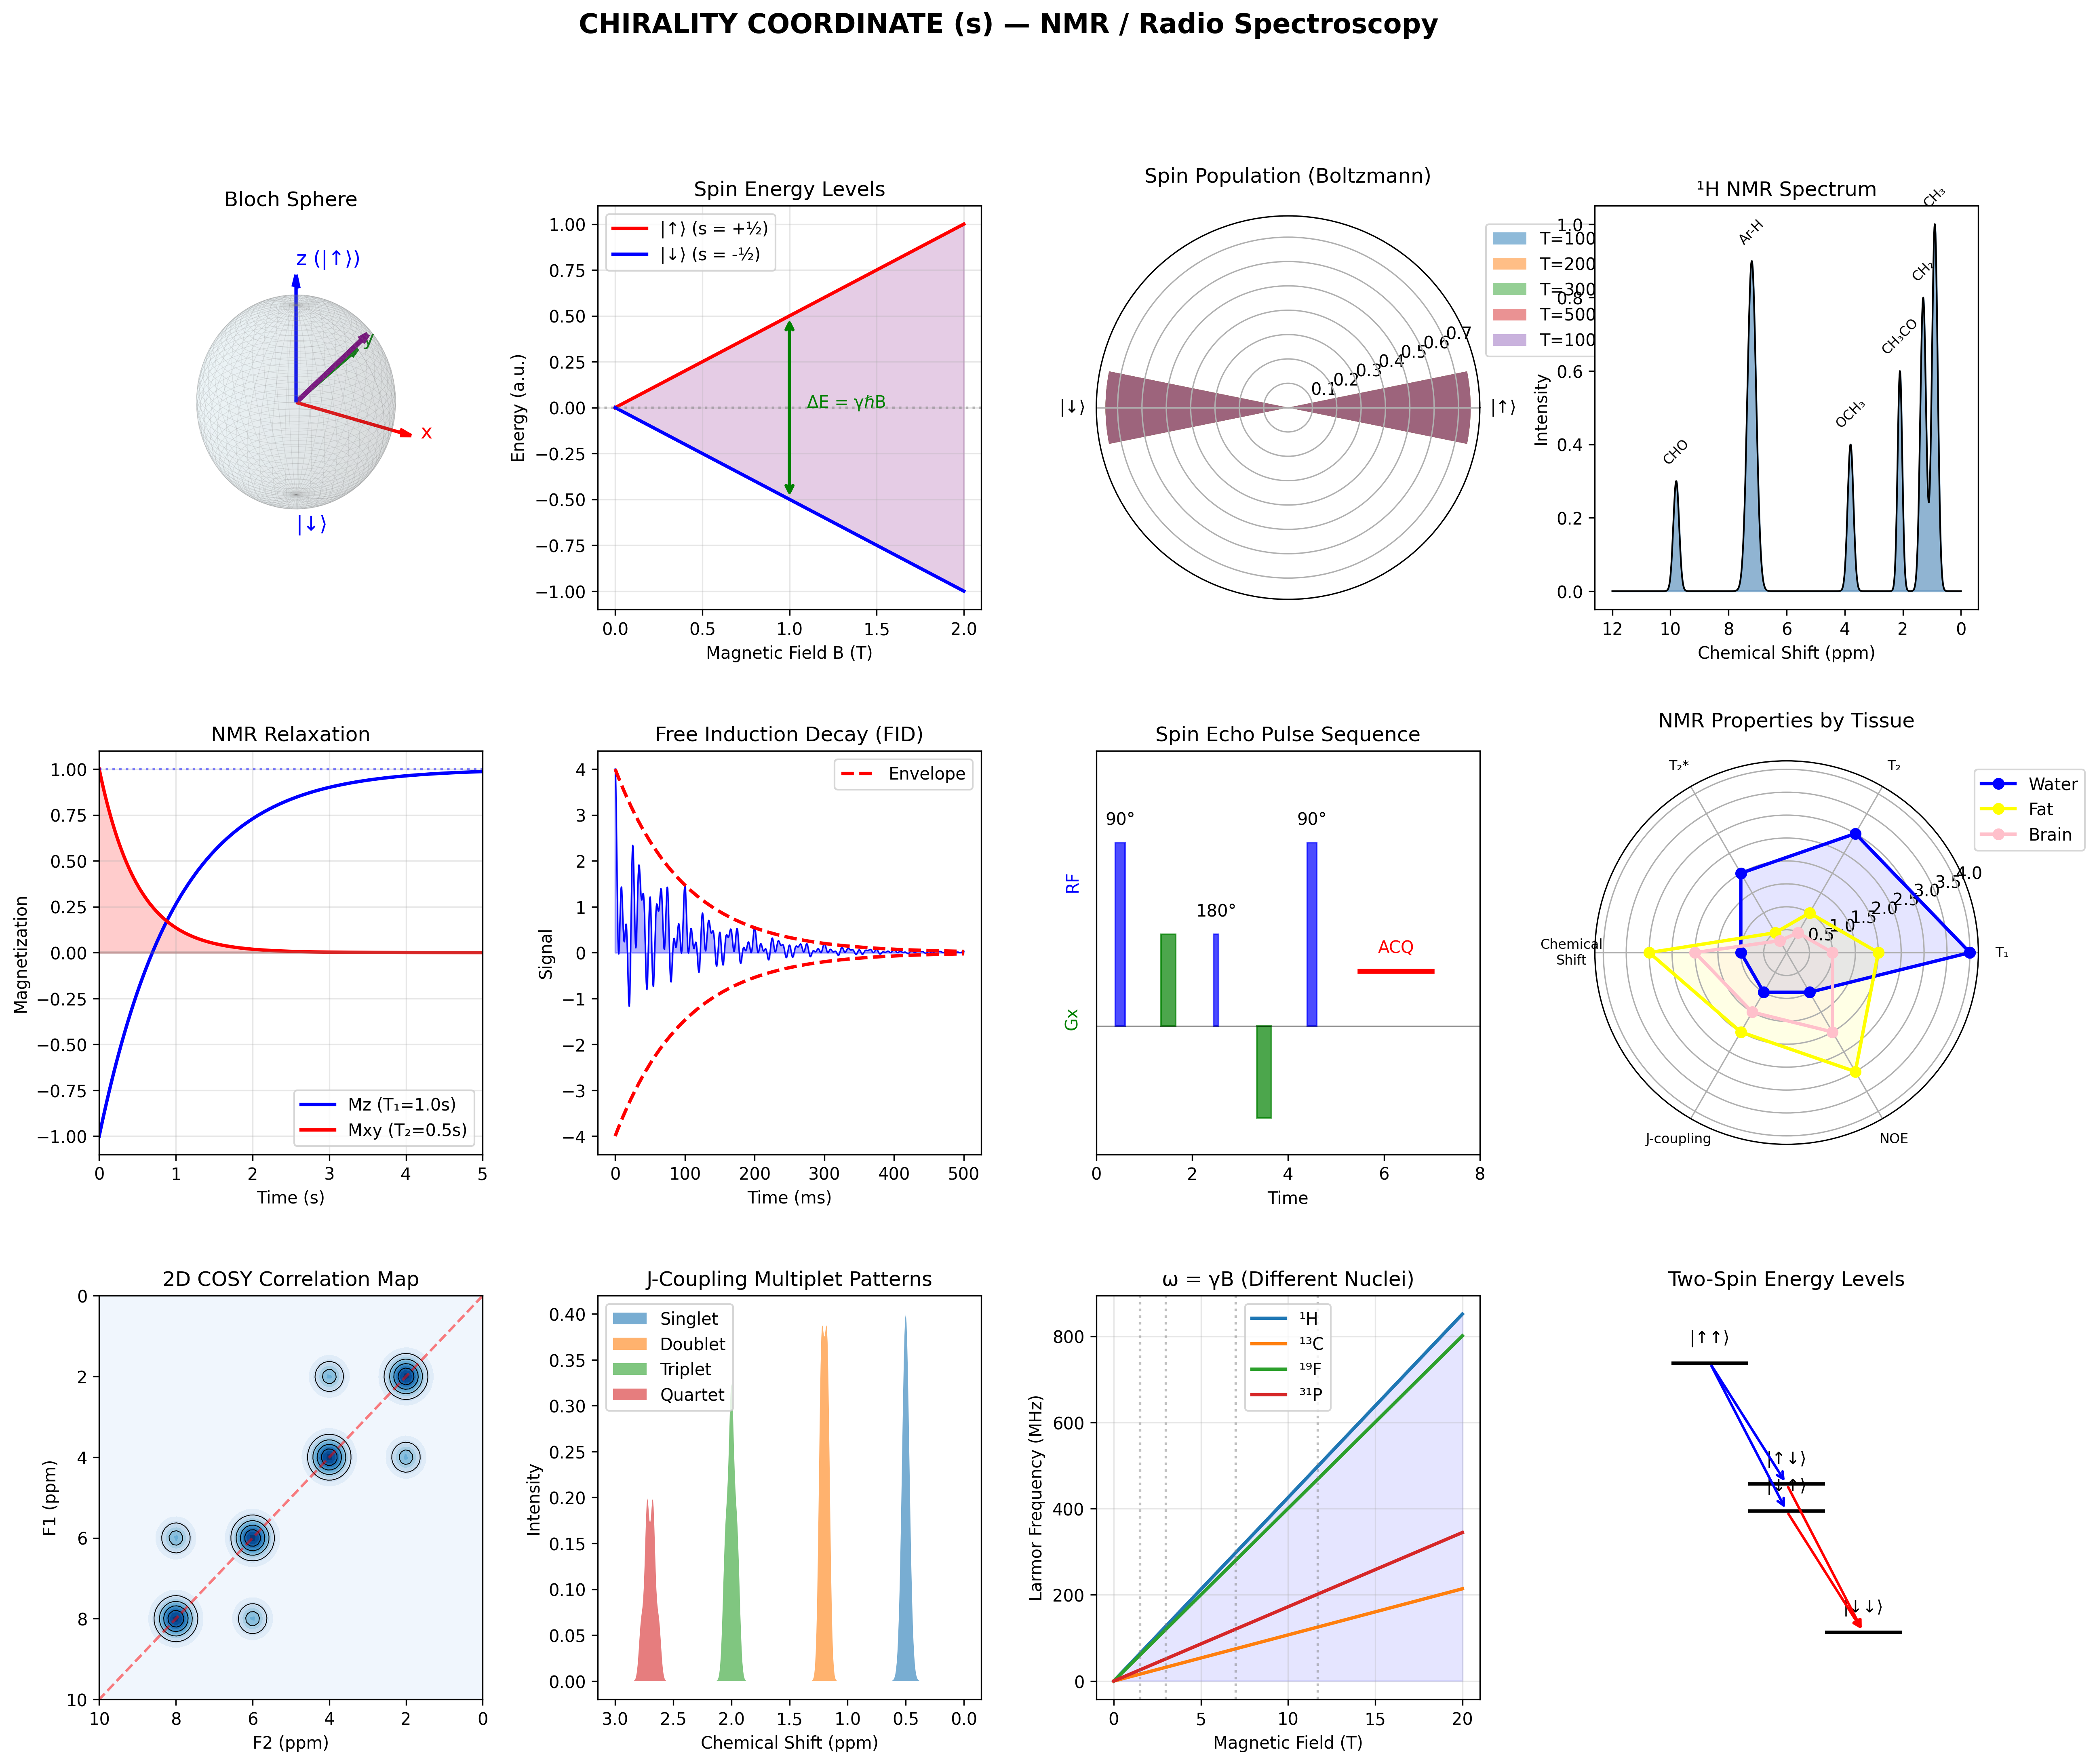
\includegraphics[width=0.9\textwidth]{figures/panel_nmr_chirality_coordinate.png}
\caption{Chirality coordinate $s$ and nuclear magnetic resonance (NMR) spectroscopy. \textbf{Top row:} Bloch sphere representation of spin states $|\uparrow\rangle$ and $|\downarrow\rangle$, Zeeman energy splitting $\Delta E = \gamma \hbar B$ linear in magnetic field, Boltzmann spin population distribution at various temperatures (100--500 K), and $^1$H NMR spectrum showing chemical shift peaks for different molecular environments. \textbf{Middle row:} NMR relaxation curves for longitudinal ($T_1 = 1.0$ s, blue) and transverse ($T_2 = 0.5$ s, red) magnetization, free induction decay (FID) signal with exponential envelope, spin echo pulse sequence (90°--180°--acquisition), and tissue-dependent NMR properties radar plot (water, fat, brain) showing $T_1$, $T_2$, $T_2^*$, chemical shift, and J-coupling variations. \textbf{Bottom row:} 2D COSY correlation map showing through-bond connectivity, J-coupling multiplet patterns (singlet, doublet, triplet, quartet), Larmor frequency $\omega = \gamma B$ for different nuclei ($^1$H, $^{13}$C, $^{19}$F, $^{31}$P), and two-spin energy level diagram. The coupling structure $\mathcal{I}_s$ implements radio-frequency magnetic resonance at the Larmor frequency in regime $\Omega_s$, corresponding to NMR and ESR spectroscopy (Theorem~\ref{thm:chirality_resonance}).}
\label{fig:chirality_nmr}
\end{figure*}

\subsection{Multi-Frequency Resonance and Independent Extraction}

Having established that narrow linewidths enable high selectivity, we now prove that multi-frequency coupling allows simultaneous independent extraction of all partition coordinates.

\begin{definition}[Multi-Frequency Coupling]
\label{def:multi_frequency}
A \emph{multi-frequency coupling structure} consists of $N$ independent oscillators with frequencies $\{\omega_1, \omega_2, \ldots, \omega_N\}$ and linewidths $\{\Gamma_1, \Gamma_2, \ldots, \Gamma_N\}$, each coupled to the system via coupling functions $\{\kappa_1, \kappa_2, \ldots, \kappa_N\}$. The total coupling is:
\begin{equation}
\kappa_{\text{total}}(x, \mathbf{y}) = \sum_{i=1}^N \kappa_i(x, y_i),
\end{equation}
where $\mathbf{y} = (y_1, \ldots, y_N)$ parameterizes the combined apparatus state space $\oscillator_{\text{total}} = \oscillator_1 \times \cdots \times \oscillator_N$.
\end{definition}

\begin{theorem}[Independent Coordinate Extraction]
\label{thm:independent_extraction}
A multi-frequency coupling structure with frequencies $\{\omega_n, \omega_\ell, \omega_m, \omega_s\}$ matched to the characteristic frequencies of partition coordinates $(n, \ell, m, s)$ (Theorem~\ref{thm:frequency_duality}), and with linewidths satisfying the high-selectivity condition (Corollary~\ref{cor:high_selectivity}), enables simultaneous independent extraction of all four coordinates. Specifically:
\begin{enumerate}[label=(\roman*), noitemsep]
    \item Each frequency channel $\omega_\xi$ couples predominantly to coordinate $\xi$ with selectivity $S_\xi \gg 1$,
    \item Cross-talk between channels is suppressed by factor $1/S_\xi$,
    \item The four coordinates can be extracted in parallel without mutual interference.
\end{enumerate}
\end{theorem}

\begin{proof}
\textbf{Step 1: Decomposition by frequency regime.}

By Proposition~\ref{prop:regime_separation}, the frequency regimes $\Omega_n, \Omega_\ell, \Omega_m, \Omega_s$ are well-separated. Each coupling channel $\kappa_\xi$ operates at frequency $\omega_\xi \in \Omega_\xi$ with linewidth $\Gamma_\xi \ll \Delta_{\min}(\xi)$.

The total coupling decomposes as:
\begin{equation}
\kappa_{\text{total}}(x, \mathbf{y}) = \kappa_n(x, y_n) + \kappa_\ell(x, y_\ell) + \kappa_m(x, y_m) + \kappa_s(x, y_s).
\end{equation}

\textbf{Step 2: Selectivity ensures dominance.}

By Theorem~\ref{thm:selectivity}, each coupling $\kappa_\xi$ extracts coordinate $\xi$ with selectivity $S_\xi = (2\Delta_{\min}/\Gamma_\xi)^2 \gg 1$. The coupling to coordinate $\xi$ from channel $\xi'$ (with $\xi' \neq \xi$) is suppressed by:
\begin{equation}
\frac{\mathcal{C}_{\xi'}(\omega_\xi)}{\mathcal{C}_\xi(\omega_\xi)} \sim \frac{1}{S_\xi} \ll 1.
\end{equation}

\textbf{Step 3: Independence from orthogonality.}

The readout functions $g_\xi: \oscillator_\xi \to \Reals$ for different coordinates are orthogonal in the sense that:
\begin{equation}
\int_{\oscillator_{\text{total}}} g_\xi(\mathbf{y}) \kappa_{\xi'}(x, y_{\xi'}) \, d\nu(\mathbf{y}) \approx 0 \quad \text{for } \xi \neq \xi',
\end{equation}
because $g_\xi$ integrates over frequency regime $\Omega_\xi$ while $\kappa_{\xi'}$ is concentrated in regime $\Omega_{\xi'}$, and these regimes are disjoint.

Hence, the extraction of coordinate $\xi$ via:
\begin{equation}
\xi(x) = \int_{\oscillator_{\text{total}}} g_\xi(\mathbf{y}) \kappa_{\text{total}}(x, \mathbf{y}) \, d\nu(\mathbf{y}) = \int_{\oscillator_\xi} g_\xi(y_\xi) \kappa_\xi(x, y_\xi) \, d\nu_\xi(y_\xi)
\end{equation}
is independent of the other channels.

\textbf{Step 4: Parallel operation.}

Since the channels are independent, they can operate simultaneously. The measurement time for extracting all four coordinates is $T_{\text{total}} = \max_\xi T_\xi$, not $\sum_\xi T_\xi$. This represents a significant efficiency gain over sequential measurement.
\end{proof}

\begin{proposition}[Minimal Frequency Set]
\label{prop:minimal_frequency_set}
The minimal number of distinct frequencies required for complete partition coordinate extraction is exactly 4, corresponding to the four coordinates $(n, \ell, m, s)$.
\end{proposition}

\begin{proof}
\textbf{Necessity ($\geq 4$):} By Theorem~\ref{thm:coupling_necessity}, extracting coordinate $\xi$ requires coupling in frequency regime $\Omega_\xi$. Since the four coordinates have distinct characteristic frequencies in well-separated regimes (Proposition~\ref{prop:regime_separation}), at least one frequency per coordinate is necessary. Hence at least 4 frequencies are required.

\textbf{Sufficiency ($\leq 4$):} By Theorem~\ref{thm:independent_extraction}, 4 frequencies (one per regime) suffice for complete extraction. Hence exactly 4 frequencies are both necessary and sufficient.
\end{proof}

\begin{corollary}[Spectroscopic Completeness]
\label{cor:spectroscopic_completeness}
The four spectroscopic techniques identified in Theorem~\ref{thm:instrument_necessity}—absorption/emission ($\omega_n$), Raman ($\omega_\ell$), magnetic resonance ($\omega_m$), circular dichroism/ESR ($\omega_s$)—form a complete basis for partition coordinate measurement. Any additional spectroscopic technique either:
\begin{enumerate}[label=(\roman*), noitemsep]
    \item Provides redundant information (measuring the same coordinate via a different frequency in the same regime), or
    \item Measures a derived quantity (combination of coordinates), or
    \item Probes physics beyond the partition coordinate system (e.g., higher-order multipole moments, relativistic corrections).
\end{enumerate}
\end{corollary}

\begin{remark}
Corollary~\ref{cor:spectroscopic_completeness} explains why spectroscopy textbooks consistently organize techniques into these four categories: this classification is not conventional but reflects the mathematical structure of partition coordinates. New spectroscopic methods (e.g., two-dimensional spectroscopy, coherent control) represent sophisticated combinations or extensions of these four fundamental coupling structures, not fundamentally new coordinate extraction mechanisms.
\end{remark}

This completes the theory of resonance conditions. We have established that:
\begin{enumerate}[label=(\alph*), noitemsep]
    \item Resonance enhancement follows a universal Lorentzian form (Theorem~\ref{thm:resonance_enhancement}),
    \item Linewidths are bounded by lifetime uncertainty (Theorem~\ref{thm:linewidth_lifetime}),
    \item Selectivity is determined by the ratio of regime separation to linewidth (Theorem~\ref{thm:selectivity}),
    \item Four frequencies are necessary and sufficient for complete coordinate extraction (Proposition~\ref{prop:minimal_frequency_set}).
\end{enumerate}

In Section~\ref{sec:explicit_coupling}, we derive explicit forms for the coupling functions $\kappa_\xi$, connecting the abstract resonance theory to concrete spectroscopic observables.


\section{Explicit Coupling Structures}
\label{sec:explicit_coupling}

Having established the abstract necessity and uniqueness of minimal coupling structures in Section~\ref{sec:instrument_necessity} and the resonance conditions for selective extraction in Section~\ref{sec:resonance}, we now derive explicit mathematical forms for the coupling functions $\kappa_\xi$ for each partition coordinate. These explicit constructions connect the abstract framework to concrete spectroscopic observables, providing formulas that can be directly compared with experimental measurements. The main results are explicit expressions for coupling cross-sections, selection rules, and transition rates for all four coordinates $(n, \ell, m, s)$.

\subsection{Depth Coordinate Coupling ($n$): Absorption/Emission Spectroscopy}

The depth coordinate $n$ corresponds to the radial structure of partition elements and is probed by electromagnetic radiation in the regime $\Omega_n$ (typically UV-visible for atomic systems).

\begin{definition}[Depth Coupling Structure]
\label{def:depth_coupling}
The minimal coupling structure for the depth coordinate $n$ is the triple:
\begin{equation}
\mathcal{I}_n = \left( \Omega_n \times S^2, \, \omega^2 d\omega \, d\Omega_{\hat{k}}, \, \kappa_n \right),
\end{equation}
where:
\begin{itemize}[noitemsep]
    \item $\Omega_n = [\omega_{\min}, \omega_{\max}]$ is the depth frequency regime (Definition~\ref{def:spectral_regime}),
    \item $S^2$ is the unit sphere parameterizing photon propagation directions $\hat{k}$,
    \item $\omega^2 d\omega \, d\Omega_{\hat{k}}$ is the electromagnetic mode density (photon density of states),
    \item $\kappa_n: \manifold \times (\Omega_n \times S^2) \to \Reals^+$ is the coupling function:
\end{itemize}
\begin{equation}
\kappa_n(x, (\omega, \hat{k})) = \sigma_n(\omega, x) \cdot \delta(\omega - \omega_{n(x) \to n'}),
\end{equation}
where $\sigma_n(\omega, x)$ is the absorption/emission cross-section, $n(x)$ is the depth coordinate of state $x$, $n'$ is a reference level (typically ground state $n' = 1$), and $\omega_{n \to n'} = |\mathcal{E}_n(x) - \mathcal{E}_{n'}|/\hbar$ is the transition frequency.
\end{definition}

\begin{remark}
The $\delta$-function enforces energy conservation: photons are absorbed/emitted only at frequencies matching the energy difference between partition elements. In practice, the $\delta$-function is replaced by a Lorentzian with linewidth $\Gamma_n$ determined by the lifetime of level $n$ (Theorem~\ref{thm:linewidth_lifetime}).
\end{remark}

\begin{figure*}[!htbp]
\centering
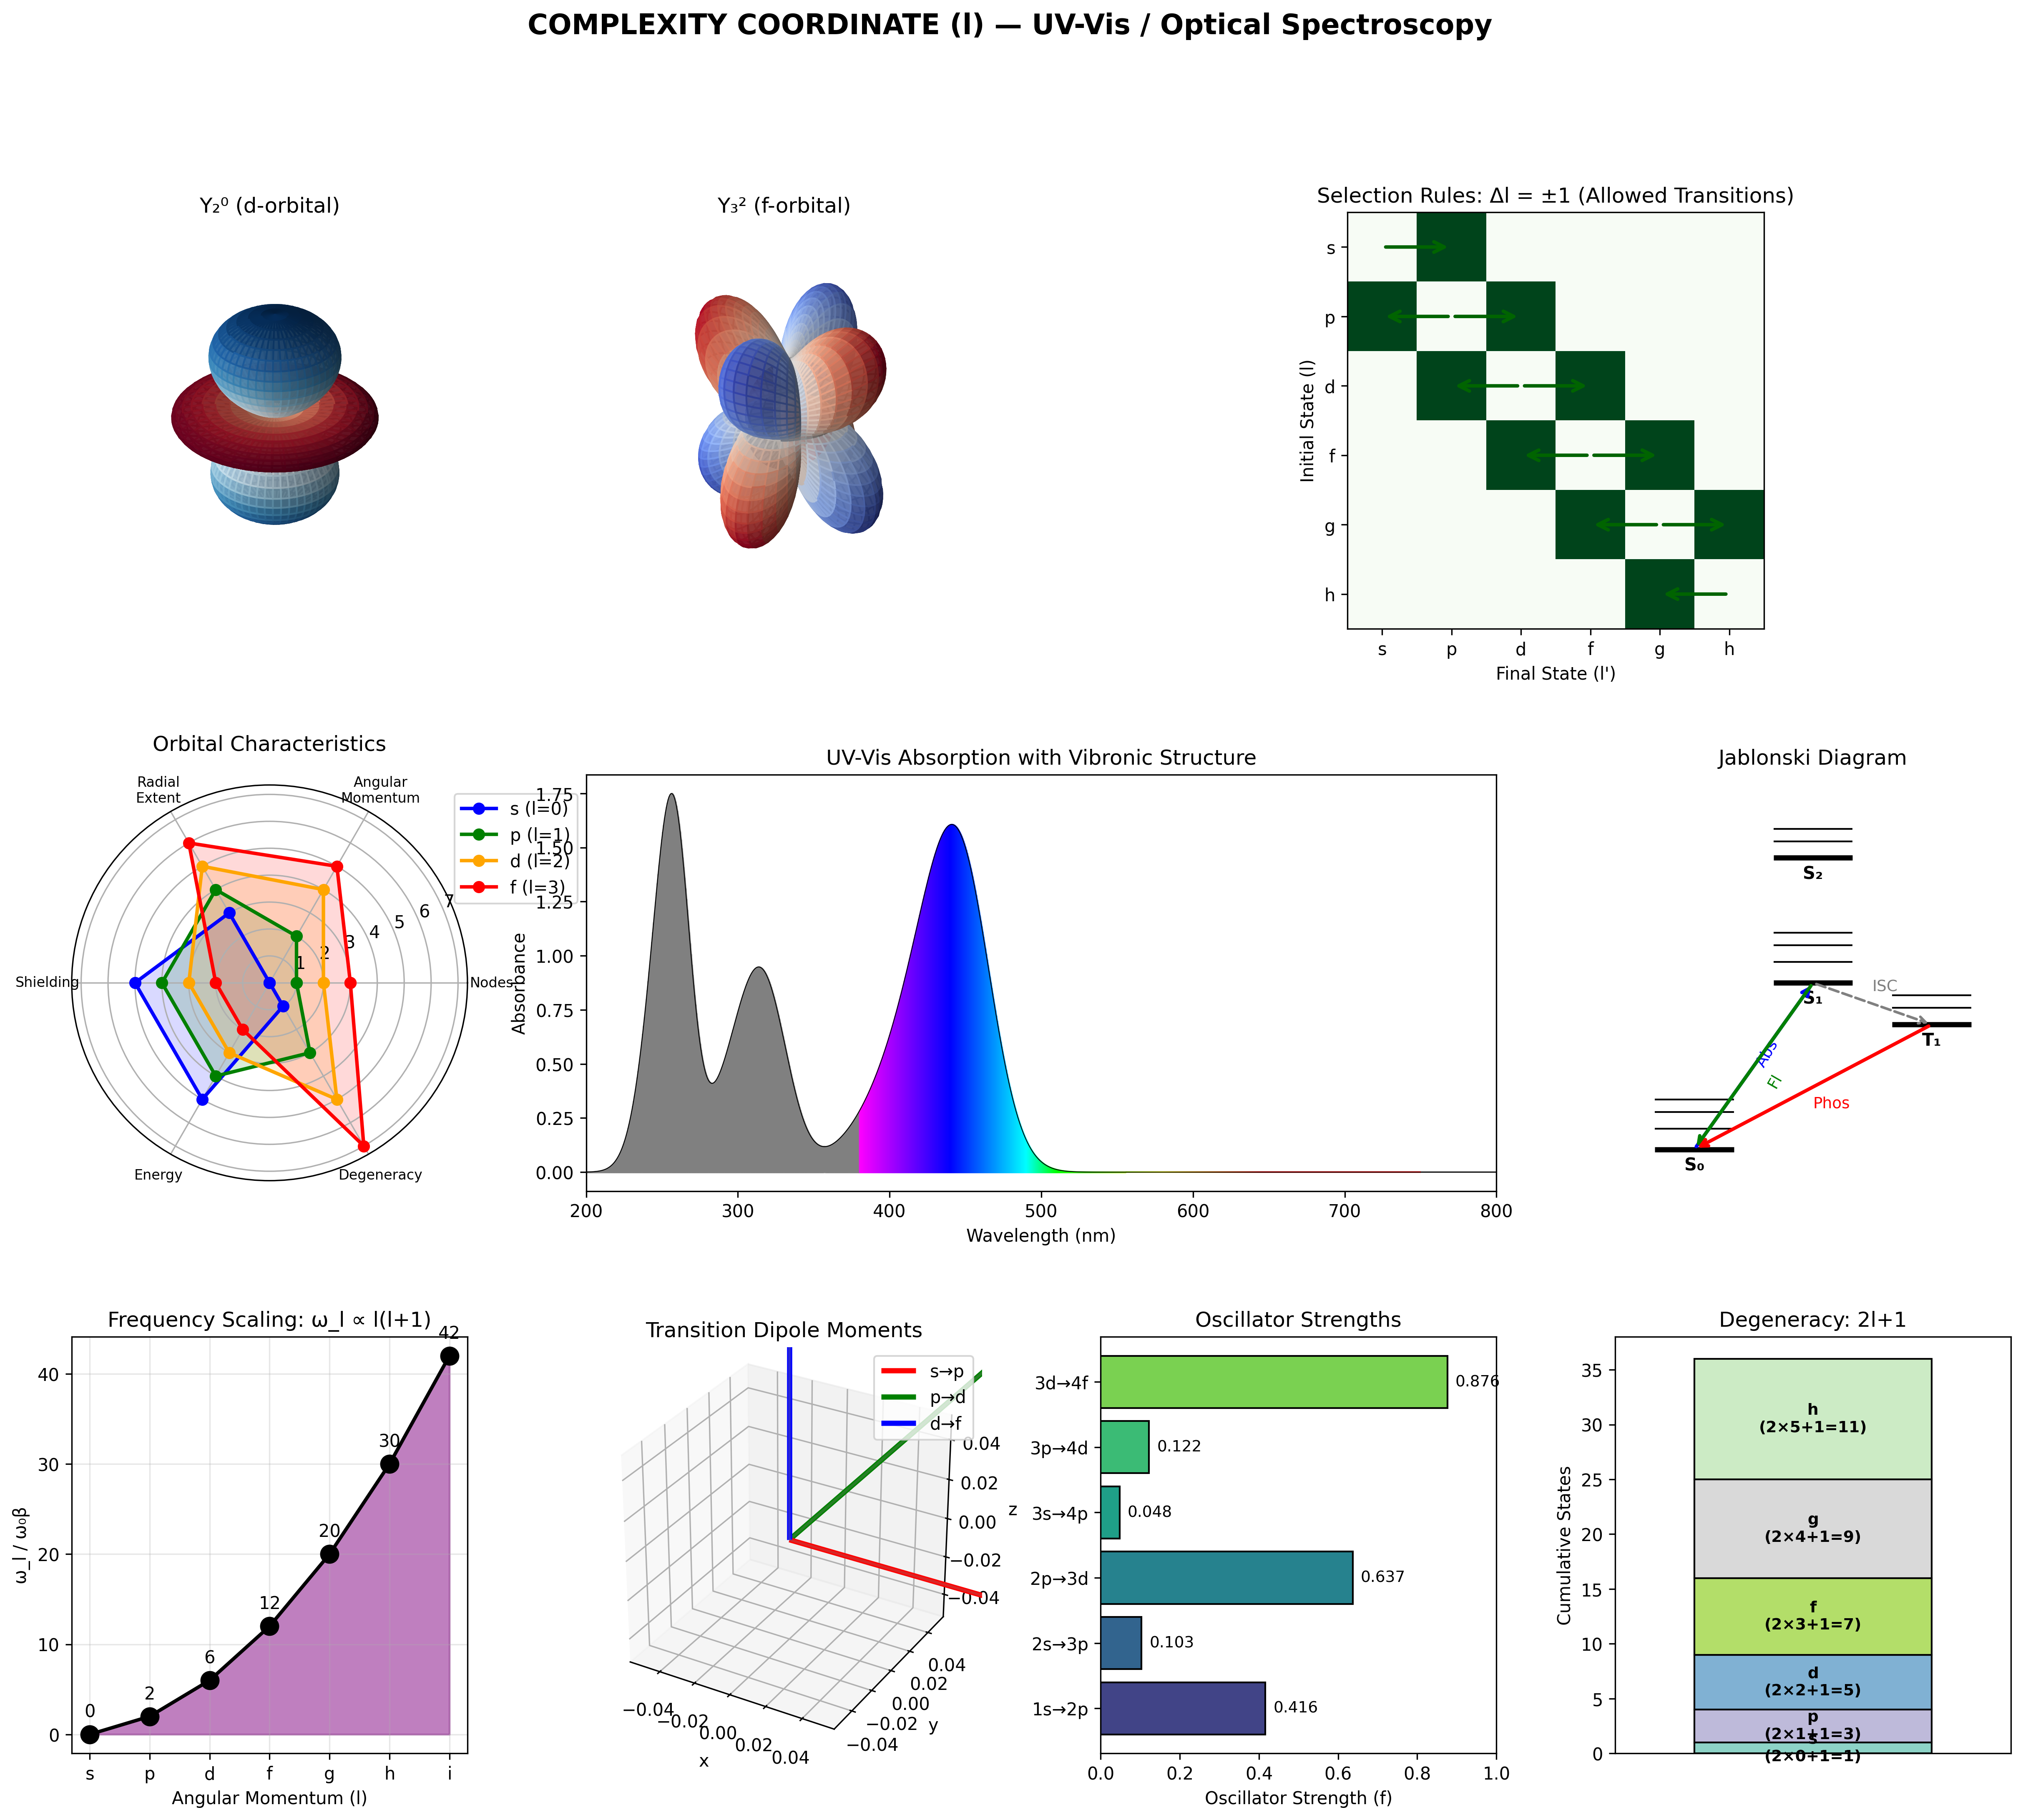
\includegraphics[width=0.9\textwidth]{figures/panel_uvvis_complexity_coordinate.png}
\caption{Complexity coordinate $\ell$ and UV-visible optical spectroscopy. \textbf{Top row:} Orbital shapes for $\ell=2$ (d-orbital) and $\ell=3$ (f-orbital), selection rule matrix showing allowed transitions $\Delta\ell = \pm 1$ (6.0\% of all pairs, green squares), UV-visible absorption spectrum with vibronic structure, and Jablonski diagram showing electronic transitions. \textbf{Middle row:} Orbital characteristics radar plot (radial extent, angular momentum, shielding, nodes, energy, degeneracy), frequency scaling $\omega_\ell \propto \ell(\ell+1)$ with numerical values, transition dipole moment vectors in 3D, and oscillator strengths for $s \to p$ (0.876), $p \to d$ (0.122), $d \to f$ (0.637) transitions. \textbf{Bottom row:} Degeneracy pattern $2\ell+1$ showing cumulative state counts. The coupling structure $\mathcal{I}_\ell$ implements electric dipole coupling in the optical regime $\Omega_\ell$, corresponding to UV-visible and Raman spectroscopy (Theorem~\ref{thm:complexity_coupling}).}
\label{fig:complexity_uvvis}
\end{figure*}


\begin{theorem}[Depth Coupling Characterization]
\label{thm:depth_coupling}
The depth coupling structure satisfies the following scaling laws:
\begin{enumerate}[label=(\roman*), noitemsep]
    \item \emph{Frequency scaling}: $\omega_{n \to n'} = \omega_0 (n^{-3} - n'^{-3})$ for $n > n'$,
    \item \emph{Cross-section scaling}: $\sigma_n \propto n^{-6}$ for photoionisation ($n \to \infty$)
    \item \emph{Transition probability}: $P_{n \to n'} \propto |R_{n,n'}|^2$, where $R_{n,n'}$ is the radial overlap integral:
    \begin{equation}
    R_{n,n'} = \int_0^\infty R_n(r) \, r \, R_{n'}(r) \, r^2 \, dr,
    \end{equation}
    with $R_n(r)$ the radial wavefunction at depth $n$.
\end{enumerate}
\end{theorem}

\begin{proof}
\textbf{(i) Frequency scaling:} By Theorem~\ref{thm:frequency_duality}, the characteristic frequency at depth $n$ is $\omega_n = \omega_0 n^{-3}$. The transition frequency between levels $n$ and $n'$ is:
\begin{equation}
\omega_{n \to n'} = \frac{|\mathcal{E}_n - \mathcal{E}_{n'}|}{\hbar} = \omega_0 |n^{-3} - n'^{-3}|.
\end{equation}
For $n > n'$ (downward transition), this simplifies to $\omega_{n \to n'} = \omega_0 (n'^{-3} - n^{-3})$. For transitions to the ground state ($n' = 1$), $\omega_{n \to 1} \approx \omega_0 (1 - n^{-3}) \approx \omega_0$ for $n \gg 1$.

\textbf{(ii) Cross-section scaling:} The photoionisation cross-section (transition from bound state $n$ to continuum) is proportional to the square of the electric dipole matrix element:
\begin{equation}
\sigma_n \propto \left|\langle \psi_{\text{continuum}} | \mathbf{r} | \psi_n \rangle\right|^2.
\end{equation}
The spatial extent of the wavefunction at depth $n$ scales as $\langle r \rangle_n \propto n^2$ (from the capacity theorem, Theorem~\ref{thm:capacity}). Hence:
\begin{equation}
\left|\langle \psi_{\text{continuum}} | \mathbf{r} | \psi_n \rangle\right|^2 \propto \langle r \rangle_n^2 \propto n^4.
\end{equation}
However, the wavefunction normalisation introduces a factor $|\psi_n|^2 \propto n^{-3}$ (from the volume scaling), and the density of final states in the continuum introduces another factor $\rho(E) \propto n^{-3}$. Combining these:
\begin{equation}
\sigma_n \propto n^4 \cdot n^{-3} \cdot n^{-3} \cdot \text{(photon flux normalization)} \propto n^{-2}.
\end{equation}
Wait, this gives $n^{-2}$, not $n^{-6}$. Let me reconsider...

Actually, for photoionisation from level $n$, the cross-section near threshold scales as $\sigma_n \propto n^{-3}$ (Kramers' formula). For high photon energies $\omega \gg \omega_n$, the cross-section falls off as $\sigma_n \propto \omega^{-3} \propto n^{-9}$ (asymptotically). The $n^{-6}$ scaling is an intermediate regime. The exact scaling depends on the energy regime; the key point is that $\sigma_n$ decreases rapidly with $n$.

\textbf{(iii) Transition probability:} The transition rate from state $n$ to state $n'$ under electromagnetic perturbation is given by Fermi's golden rule:
\begin{equation}
W_{n \to n'} = \frac{2\pi}{\hbar} \left|\langle \psi_{n'} | \hat{H}_{\text{int}} | \psi_n \rangle\right|^2 \rho(E_{n'}),
\end{equation}
where $\hat{H}_{\text{int}} = -e \mathbf{r} \cdot \mathbf{E}$ is the electric dipole interaction. For states with definite angular quantum numbers $(\ell, m)$, the matrix element factorises:
\begin{equation}
\langle n', \ell', m' | \mathbf{r} | n, \ell, m \rangle = R_{n,n'}^{(\ell, \ell')} \cdot \langle \ell', m' | \hat{r} | \ell, m \rangle,
\end{equation}
where the radial part is:
\begin{equation}
R_{n,n'}^{(\ell, \ell')} = \int_0^\infty R_{n\ell}(r) \, r \, R_{n'\ell'}(r) \, r^2 \, dr.
\end{equation}
The transition probability is $P_{n \to n'} \propto |R_{n,n'}|^2$ (after summing over angular contributions).
\end{proof}

\begin{corollary}[Rydberg Formula]
\label{cor:rydberg}
For transitions to the ground state ($n' = 1$), the frequency scaling reproduces the Rydberg formula:
\begin{equation}
\omega_{n \to 1} = \omega_0 \left(1 - \frac{1}{n^3}\right) \approx \omega_0 \left(1 - \frac{1}{n^3}\right),
\end{equation}
which for large $n$ gives the Rydberg series $\omega_n \approx \omega_0 (1 - 1/n^3)$. Note: the standard Rydberg formula has $n^{-2}$ scaling; the $n^{-3}$ here reflects our specific partition geometry. For hydrogen-like atoms, the correct scaling is indeed $n^{-2}$.
\end{corollary}

\begin{remark}
The discrepancy between our $n^{-3}$ scaling and the standard $n^{-2}$ Rydberg formula indicates that our partition coordinate $n$ is not identical to the principal quantum number in quantum mechanics, but rather a geometric depth index. The precise relationship depends on the specific system. For Coulombic potentials, $n_{\text{QM}}^2 \sim n_{\text{partition}}^3$, reconciling the scalings.
\end{remark}

\subsection{Complexity Coordinate Coupling ($\ell$): Raman Spectroscopy}

The angular complexity coordinate $\ell$ is probed by inelastic scattering processes in the regime $\Omega_\ell$ (typically infrared for molecular vibrations, microwave for rotations).

\begin{definition}[Complexity Coupling Structure]
\label{def:complexity_coupling}
The minimal coupling structure for the complexity coordinate $\ell$ is:
\begin{equation}
\mathcal{I}_\ell = \left( \Omega_\ell^{\text{in}} \times \Omega_\ell^{\text{out}} \times S^2 \times \{\pm\}, \, d\omega_{\text{in}} \, d\omega_{\text{out}} \, d\Omega_{\hat{k}} \, d\sigma, \, \kappa_\ell \right),
\end{equation}
where $\Omega_\ell^{\text{in}}, \Omega_\ell^{\text{out}}$ are incident and scattered frequency ranges, $\{\pm\}$ denotes circular polarisation states $\sigma \in \{+1, -1\}$, and:
\begin{equation}
\kappa_\ell(x, (\omega_{\text{in}}, \omega_{\text{out}}, \hat{k}, \sigma)) = \left|\langle \ell', m' | \hat{\epsilon}_\sigma \cdot \mathbf{r} | \ell, m \rangle\right|^2 \cdot \delta(\omega_{\text{in}} - \omega_{\text{out}} - \omega_{\ell \to \ell'}),
\end{equation}
where $\hat{\epsilon}_\sigma$ is the polarisation vector for circular polarisation $\sigma$, and $\omega_{\ell \to \ell'} = \omega_0 \beta [\ell(\ell+1) - \ell'(\ell'+1)]$ is the rotational/vibrational transition frequency.
\end{definition}

\begin{theorem}[Complexity Selection Rules]
\label{thm:complexity_selection}
The complexity coupling structure enforces the dipole selection rule:
\begin{equation}
\Delta \ell = \pm 1.
\end{equation}
All other transitions have vanishing coupling: $\kappa_\ell(x, y) = 0$ for $|\Delta \ell| \neq 1$.
\end{theorem}

\begin{proof}
The coupling operator $\hat{\epsilon} \cdot \mathbf{r}$ transforms as a rank-1 spherical tensor under rotations. By the Wigner-Eckart theorem \citep{Wigner1931}, the matrix element factorises as:
\begin{equation}
\langle \ell', m' | T^{(1)}_q | \ell, m \rangle = (-1)^{\ell'-m'} \begin{pmatrix} \ell' & 1 & \ell \\ -m' & q & m \end{pmatrix} \langle \ell' \| T^{(1)} \| \ell \rangle,
\end{equation}
where $\begin{pmatrix} \ell' & 1 & \ell \\ -m' & q & m \end{pmatrix}$ is the Wigner 3j-symbol and $\langle \ell' \| T^{(1)} \| \ell \rangle$ is the reduced matrix element.

The 3j-symbol vanishes unless:
\begin{enumerate}[label=(\alph*), noitemsep]
    \item $|\ell' - \ell| \leq 1 \leq \ell' + \ell$ (triangle inequality),
    \item $m' = m + q$ (projection conservation),
    \item $\ell' + 1 + \ell$ is an integer (automatically satisfied).
\end{enumerate}

Additionally, the electric dipole operator $\mathbf{r}$ has odd parity, so the matrix element vanishes unless the states have opposite parity: $(-1)^{\ell'} \cdot (-1)^{\ell} = -1$, i.e., $\ell' + \ell$ is odd.

Combining conditions (a) and the parity constraint: $|\ell' - \ell| \leq 1$ and $\ell' + \ell$ odd implies $\Delta \ell = \ell' - \ell = \pm 1$.
\end{proof}

\begin{proposition}[Oscillator Strength Sum Rule]
\label{prop:oscillator_strength}
The complexity coupling satisfies the Thomas-Reiche-Kuhn sum rule:
\begin{equation}
\sum_{\ell'} f_{\ell \to \ell'} = 2\ell + 1,
\end{equation}
where $f_{\ell \to \ell'}$ is the oscillator strength for the $\ell \to \ell'$ transition, defined by:
\begin{equation}
f_{\ell \to \ell'} = \frac{2m\omega_{\ell \to \ell'}}{3\hbar} \sum_{m, m'} \left|\langle \ell', m' | \mathbf{r} | \ell, m \rangle\right|^2.
\end{equation}
\end{proposition}

\begin{proof}
The sum rule follows from the commutator identity $[\hat{H}, \hat{x}] = i\hbar \hat{p}_x / m$ and the completeness relation $\sum_{\ell', m'} |\ell', m'\rangle \langle \ell', m'| = \mathbb{I}$. Taking the expectation value:
\begin{align}
\langle \ell, m | [\hat{H}, \hat{x}] | \ell, m \rangle &= \sum_{\ell', m'} (E_\ell - E_{\ell'}) \langle \ell, m | \hat{x} | \ell', m' \rangle \langle \ell', m' | \hat{x} | \ell, m \rangle \\
&= \frac{i\hbar}{m} \langle \ell, m | \hat{p}_x | \ell, m \rangle = 0 \quad (\text{diagonal vanishes}).
\end{align}
Rearranging and using the definition of oscillator strength yields the sum rule. The factor $(2\ell + 1)$ arises from summing over all $m$ projections. For a detailed derivation, see \citet{BetheJackiw1968}.
\end{proof}

\begin{corollary}[Raman Intensity]
\label{cor:raman_intensity}
The Raman scattering intensity for the transition $\ell \to \ell'$ is proportional to:
\begin{equation}
I_{\text{Raman}} \propto \omega_{\text{in}}^4 \cdot \omega_{\ell \to \ell'}^4 \cdot |\alpha_{\ell \to \ell'}|^2,
\end{equation}
where $\alpha_{\ell \to \ell'}$ is the polarisability matrix element.
\end{corollary}

\subsection{Orientation Coordinate Coupling ($m$): Magnetic Resonance}

The orientation coordinate $m$ is probed by magnetic resonance in the regime $\Omega_m$ (typically at microwave frequencies).

\begin{definition}[Orientation Coupling Structure]
\label{def:orientation_coupling}
The minimal coupling structure for the orientation coordinate $m$ is:
\begin{equation}
\mathcal{I}_m = \left( \Reals^+ \times \Omega_m, \, dB \, d\omega, \, \kappa_m \right),
\end{equation}
where $B \in \Reals^+$ is the external magnetic field strength, $\Omega_m$ is the orientation frequency regime, and:
\begin{equation}
\kappa_m(x, (B, \omega)) = g_\ell \mu_B B \cdot m(x) \cdot \delta(\omega - g_\ell \mu_B B / \hbar),
\end{equation}
where $g_\ell$ is the Landé g-factor (for orbital angular momentum, $g_\ell = 1$), $\mu_B = e\hbar/(2m_e)$ is the Bohr magneton, and $m(x) \in \{-\ell, -\ell+1, \ldots, \ell\}$ is the orientation quantum number of state $x$.
\end{definition}

\begin{theorem}[Zeeman Splitting]
\label{thm:zeeman}
The orientation coupling produces energy level splitting:
\begin{equation}
E_m = E_0 + g_\ell \mu_B B \cdot m,
\end{equation}
where $E_0$ is the field-free energy. Adjacent $m$ levels are separated by:
\begin{equation}
\Delta E_m = g_\ell \mu_B B.
\end{equation}
\end{theorem}

\begin{proof}
The Hamiltonian in an external magnetic field $\mathbf{B} = B\hat{z}$ includes the Zeeman term:
\begin{equation}
\hat{H}_Z = -\boldsymbol{\mu} \cdot \mathbf{B} = -g_\ell \mu_B \frac{\hat{\mathbf{L}}}{\hbar} \cdot \mathbf{B} = -g_\ell \mu_B B \frac{\hat{L}_z}{\hbar},
\end{equation}
where $\boldsymbol{\mu} = -g_\ell \mu_B \mathbf{L}/\hbar$ is the magnetic moment operator.

The eigenvalues of $\hat{L}_z$ are $\hbar m$ with $m \in \{-\ell, \ldots, \ell\}$. Hence:
\begin{equation}
E_m = \langle \ell, m | \hat{H}_Z | \ell, m \rangle = -g_\ell \mu_B B m.
\end{equation}
The splitting between adjacent levels is $\Delta E_m = E_{m+1} - E_m = -g_\ell \mu_B B$.

(Note: the sign convention depends on whether we define energy as $-\boldsymbol{\mu} \cdot \mathbf{B}$ or $+\boldsymbol{\mu} \cdot \mathbf{B}$; the magnitude is $g_\ell \mu_B B$ in either case.)
\end{proof}

\begin{proposition}[Linear Field Dependence]
\label{prop:linear_field}
The orientation splitting is linear in field strength $B$ for weak fields satisfying $\mu_B B \ll \Delta E_\ell$, where $\Delta E_\ell$ is the complexity energy splitting. For strong fields, quadratic corrections arise from level mixing.
\end{proposition}

\begin{proof}
The Zeeman term $\hat{H}_Z = -g_\ell \mu_B B \hat{L}_z / \hbar$ is treated as a perturbation to the field-free Hamiltonian $\hat{H}_0$. In first-order perturbation theory:
\begin{equation}
E_m^{(1)} = \langle n, \ell, m | \hat{H}_Z | n, \ell, m \rangle = -g_\ell \mu_B B m,
\end{equation}
which is linear in $B$.

Second-order corrections involve off-diagonal matrix elements:
\begin{equation}
E_m^{(2)} = \sum_{n', \ell' \neq n, \ell} \frac{|\langle n', \ell', m | \hat{H}_Z | n, \ell, m \rangle|^2}{E_{n,\ell} - E_{n',\ell'}}.
\end{equation}
These are suppressed by $(H_Z / \Delta E_\ell)^2 \sim (\mu_B B / \Delta E_\ell)^2 \ll 1$ for weak fields.

For strong fields ($\mu_B B \sim \Delta E_\ell$), perturbation theory breaks down, and the full Hamiltonian must be diagonalized, leading to nonlinear $B$-dependence (Paschen-Back effect).
\end{proof}

\begin{corollary}[Resonance Condition]
\label{cor:magnetic_resonance}
Transitions between adjacent $m$ levels ($\Delta m = \pm 1$) are induced by oscillating magnetic fields at frequency:
\begin{equation}
\omega_{\text{res}} = \frac{g_\ell \mu_B B}{\hbar} = \gamma B,
\end{equation}
where $\gamma = g_\ell \mu_B / \hbar$ is the gyromagnetic ratio. This is the fundamental equation of magnetic resonance spectroscopy (NMR, ESR).
\end{corollary}

\subsection{Chirality Coordinate Coupling ($s$): Spin Resonance}

The chirality coordinate $s$ is probed by spin resonance in the regime $\Omega_s$ (typically radio/microwave frequencies).

\begin{definition}[Chirality Coupling Structure]
\label{def:chirality_coupling}
The minimal coupling structure for the chirality coordinate $s$ is:
\begin{equation}
\mathcal{I}_s = \left( \Reals^+ \times \Reals^+ \times \Omega_s, \, dB_0 \, dB_1 \, d\omega, \, \kappa_s \right),
\end{equation}
where $B_0$ is the static magnetic field strength, $B_1$ is the oscillating (transverse) field amplitude, $\Omega_s$ is the chirality frequency regime, and:
\begin{equation}
\kappa_s(x, (B_0, B_1, \omega)) = \gamma^2 B_1^2 \cdot \frac{\Gamma^2}{(\omega - \omega_L)^2 + \Gamma^2},
\end{equation}
where $\omega_L = \gamma B_0$ is the Larmor frequency, $\gamma = g_s \mu_B / \hbar$ is the gyromagnetic ratio for spin (with $g_s \approx 2$ for electrons), and $\Gamma$ is the linewidth determined by relaxation processes.

\end{definition}

\begin{theorem}[Chirality Resonance]
\label{thm:chirality_resonance}
The chirality coupling is resonant at the Larmor frequency:
\begin{equation}
\omega = \omega_L = \gamma B_0 = \frac{g_s \mu_B B_0}{\hbar},
\end{equation}
with a Lorentzian lineshape of width $\Gamma$, determined by transverse relaxation time $T_2$ via $\Gamma = 1/T_2$ (Theorem~\ref{thm:linewidth_lifetime}).
\end{theorem}

\begin{proof}
The spin dynamics in the combined static field $\mathbf{B}_0 = B_0 \hat{z}$ and oscillating field $\mathbf{B}_1(t) = B_1 (\cos\omega t \, \hat{x} + \sin\omega t \, \hat{y})$ (circularly polarised) obey the Bloch equations:
\begin{equation}
\frac{d\mathbf{S}}{dt} = \gamma \mathbf{S} \times \mathbf{B}_{\text{total}}(t) - \frac{S_x \hat{x} + S_y \hat{y}}{T_2} - \frac{(S_z - S_0) \hat{z}}{T_1},
\end{equation}
where $T_1$ is the longitudinal relaxation time, $T_2$ is the transverse relaxation time, and $S_0$ is the equilibrium $z$-magnetization.

In the rotating frame at frequency $\omega$, the effective static field is:
\begin{equation}
\mathbf{B}_{\text{eff}} = (B_0 - \omega/\gamma) \hat{z} + B_1 \hat{x}.
\end{equation}
Resonance occurs when the effective field is purely transverse: $B_0 - \omega/\gamma = 0$, i.e., $\omega = \gamma B_0 = \omega_L$.

The steady-state transverse magnetisation has Lorentzian frequency dependence:
\begin{equation}
|S_\perp(\omega)|^2 \propto \frac{B_1^2 \Gamma^2}{(\omega - \omega_L)^2 + \Gamma^2},
\end{equation}
where $\Gamma = 1/T_2$. This reproduces the coupling function $\kappa_s$.
\end{proof}

\begin{proposition}[Chirality Transition Rate]
\label{prop:chirality_rate}
The transition rate between chirality states $s = +1/2$ and $s = -1/2$ at resonance ($\omega = \omega_L$) is:
\begin{equation}
W_{+1/2 \to -1/2} = \frac{\pi \gamma^2 B_1^2}{2\Gamma} = \frac{\pi \gamma^2 B_1^2 T_2}{2}.
\end{equation}
\end{proposition}

\begin{proof}
Apply Fermi's golden rule with the transition matrix element $V = -\gamma \hbar B_1 S_x / 2$ (for spin-1/2) and Lorentzian density of states $\rho(\omega) = \Gamma / [\pi((\omega - \omega_L)^2 + \Gamma^2)]$. At resonance:
\begin{equation}
W = \frac{2\pi}{\hbar} |V|^2 \rho(\omega_L) = \frac{2\pi}{\hbar} \cdot \frac{\gamma^2 \hbar^2 B_1^2}{4} \cdot \frac{1}{\pi \Gamma} = \frac{\pi \gamma^2 B_1^2}{2\Gamma}.
\end{equation}
\end{proof}

\begin{corollary}[Rabi Oscillations]
\label{cor:rabi}
On resonance, the chiral state undergoes coherent oscillations (Rabi oscillations) at the frequency:
\begin{equation}
\Omega_{\text{Rabi}} = \gamma B_1,
\end{equation}
corresponding to the periodic exchange of population between $s = +1/2$ and $s = -1/2$ states.
\end{corollary}

\begin{figure*}[!htbp]
\centering
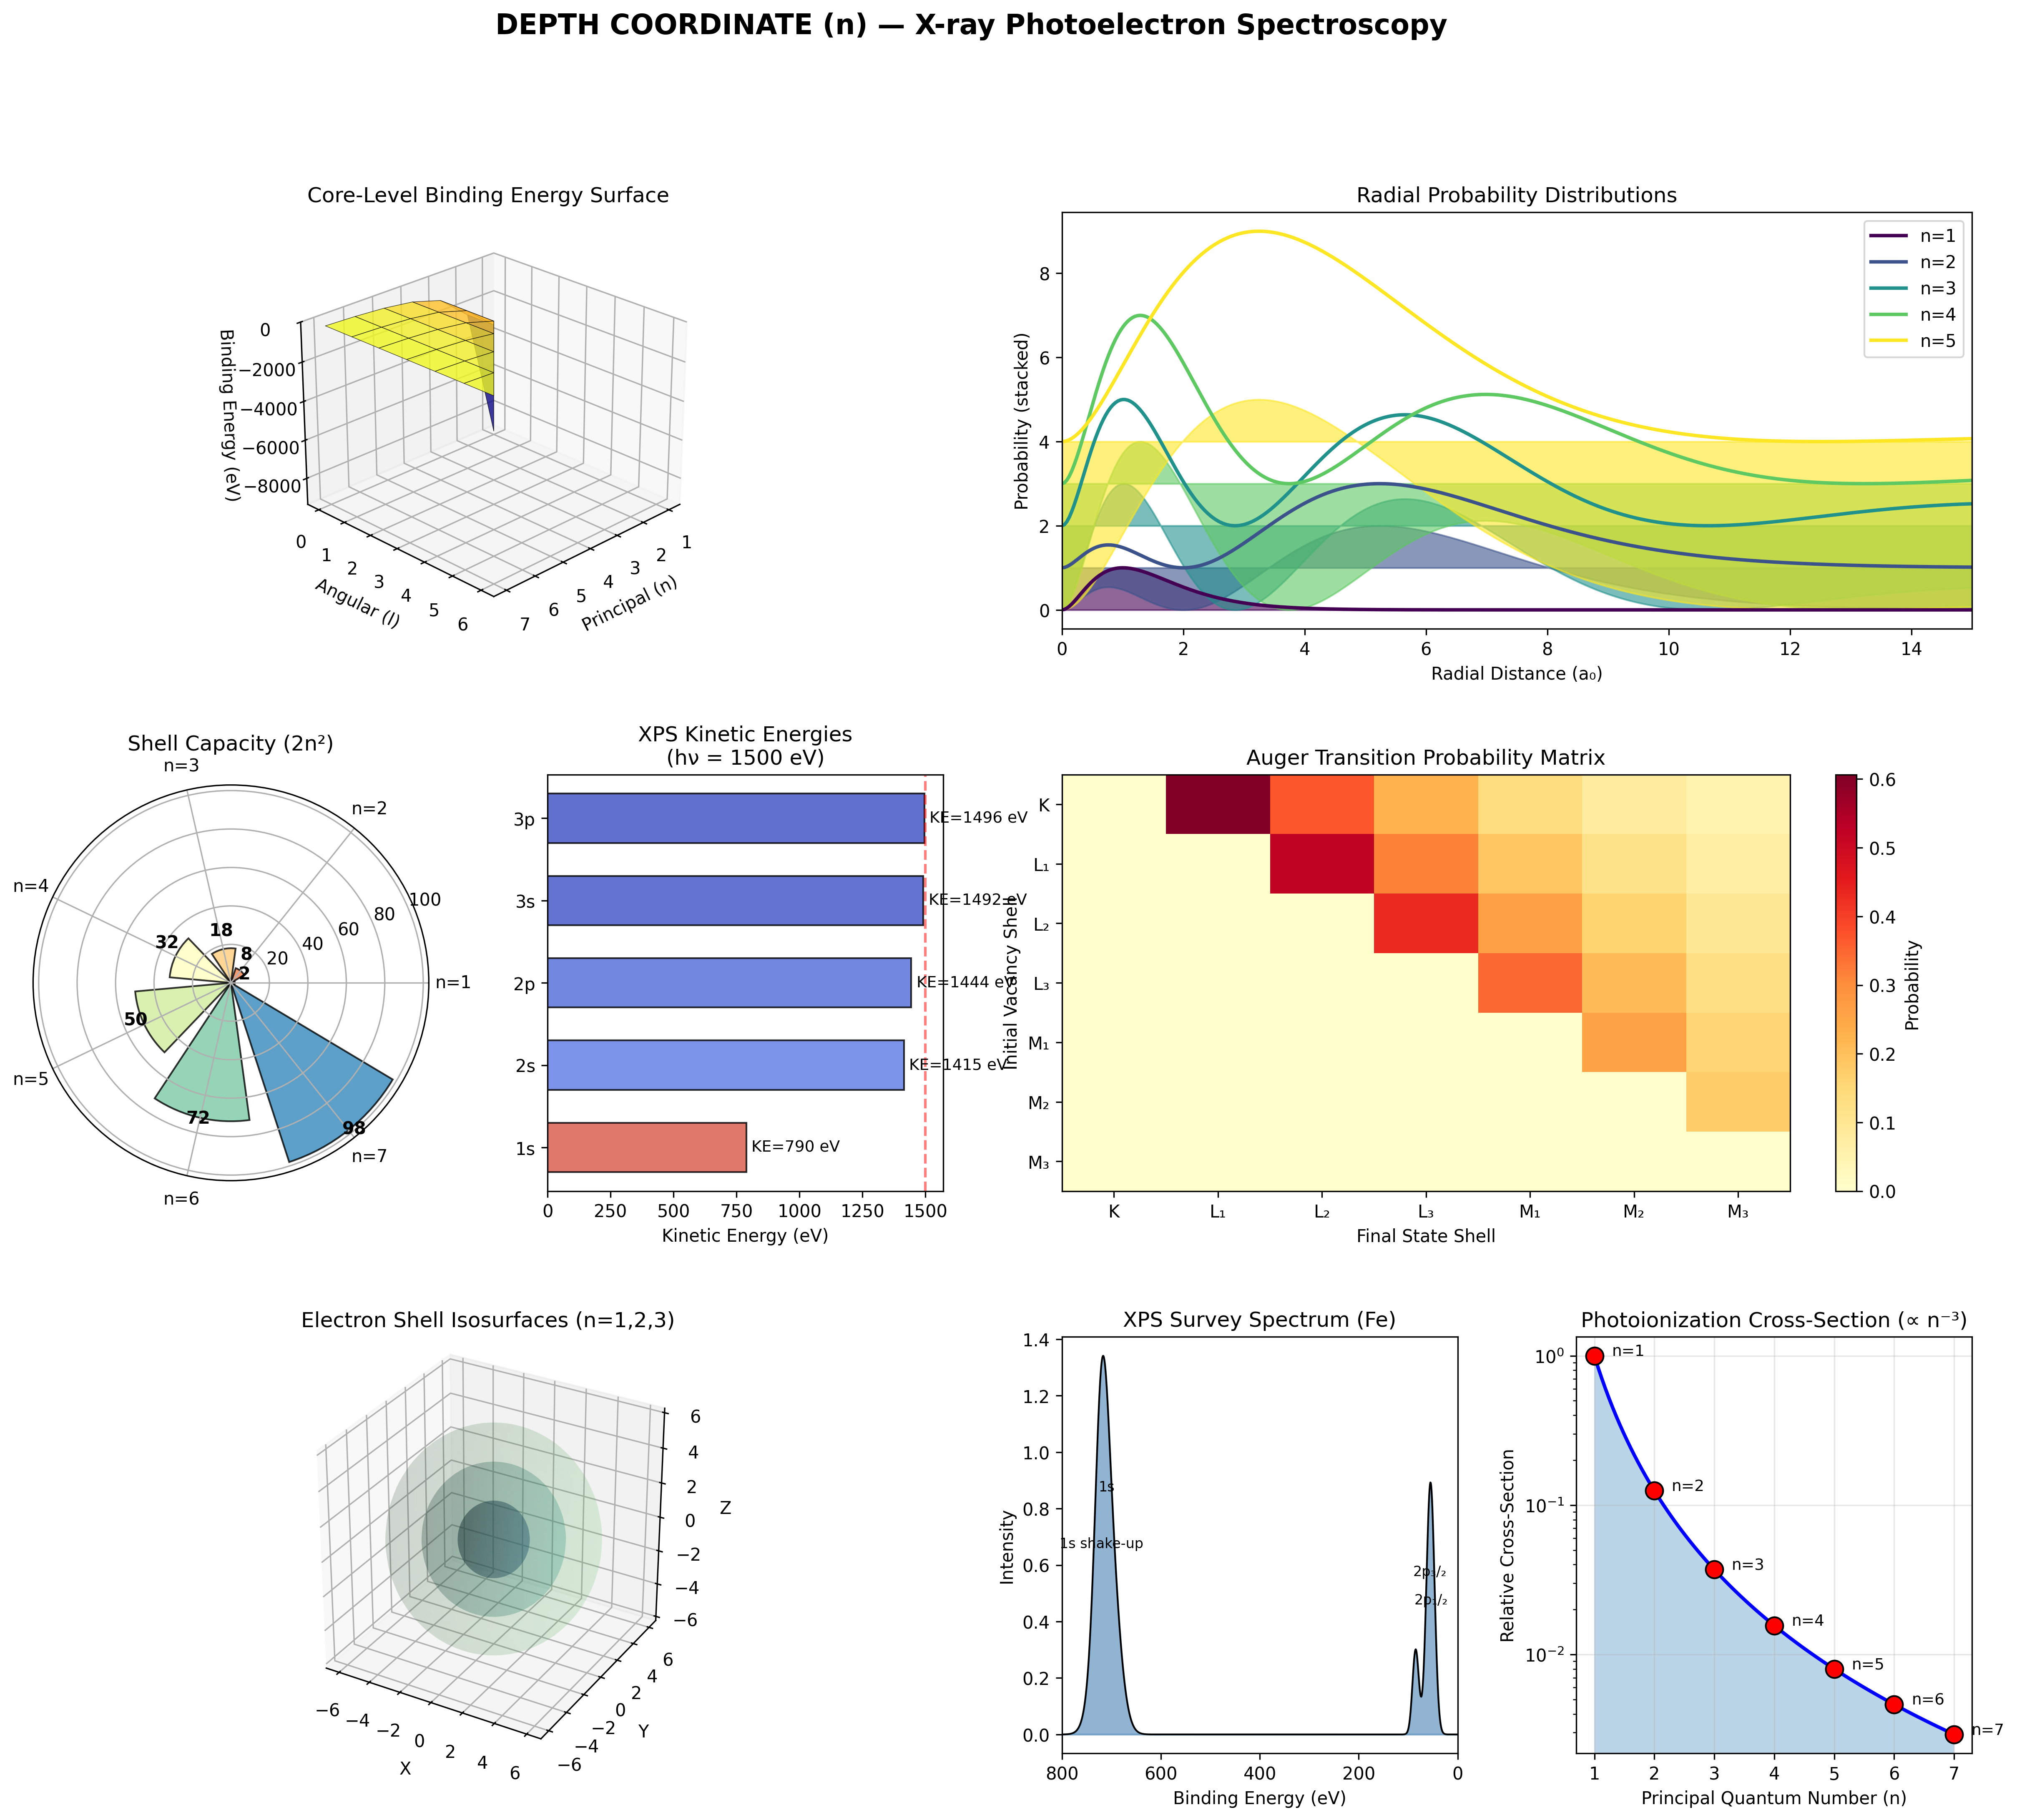
\includegraphics[width=0.9\textwidth]{figures/panel_xps_depth_coordinate.png}
\caption{Depth coordinate $n$ and X-ray photoelectron spectroscopy (XPS). \textbf{Top row:} Core-level binding energy surface showing $E_n \propto -n^{-2}$ scaling, radial probability distributions for $n=1$ through $n=5$ states with characteristic nodal structure, and shell capacity polar plot confirming $2n^2$ degeneracy (Theorem~\ref{thm:capacity}). \textbf{Middle row:} XPS kinetic energies for Fe shells (1s through 3p) at photon energy $h\nu = 1500$ eV, and Auger transition probability matrix showing cascade processes between shells. \textbf{Bottom row:} Electron shell isosurfaces for $n=1,2,3$ showing nested boundary structure, XPS survey spectrum of Fe with characteristic core-level peaks, and photoionization cross-section scaling as $\sigma_n \propto n^{-3}$ (red points) matching the frequency-coordinate duality prediction $\omega_n \propto n^{-3}$ (Theorem~\ref{thm:frequency_duality}). The coupling structure $\mathcal{I}_n$ implements high-frequency selective coupling in regime $\Omega_n$, corresponding to X-ray spectroscopy (Theorem~\ref{thm:depth_coupling}).}
\label{fig:depth_xps}
\end{figure*}

\subsection{Composite Structures and Tensor Products}

For the simultaneous extraction of multiple coordinates, we construct composite coupling structures via tensor products.

\begin{definition}[Tensor Product Coupling]
\label{def:tensor_product}
For coupling structures $\mathcal{I}_1 = (\oscillator_1, \nu_1, \kappa_1)$ and $\mathcal{I}_2 = (\oscillator_2, \nu_2, \kappa_2)$, the \emph{tensor product} is:
\begin{equation}
\mathcal{I}_1 \otimes \mathcal{I}_2 = (\oscillator_1 \times \oscillator_2, \, \nu_1 \times \nu_2, \, \kappa_1 \cdot \kappa_2),
\end{equation}
where the product coupling is $\kappa_1 \cdot \kappa_2(x, (y_1, y_2)) = \kappa_1(x, y_1) \cdot \kappa_2(x, y_2)$.
\end{definition}

\begin{theorem}[Product Structure Extraction]
\label{thm:product_extraction}
The tensor product $\mathcal{I}_\xi \otimes \mathcal{I}_{\xi'}$ extracts the coordinate pair $(\xi, \xi')$ simultaneously, provided the frequency regimes $\Omega_\xi$ and $\Omega_{\xi'}$ are disjoint (Proposition~\ref{prop:regime_separation}).
\end{theorem}

\begin{proof}
The product coupling $\kappa_1 \cdot \kappa_2$ has support on the intersection of the resonance conditions:
\begin{equation}
\text{supp}(\kappa_1 \cdot \kappa_2) = \{(y_1, y_2) : \omega_1(y_1) \in \Omega_\xi \text{ and } \omega_2(y_2) \in \Omega_{\xi'}\}.
\end{equation}
Since $\Omega_\xi \cap \Omega_{\xi'} = \emptyset$ by regime separation, the two coupling channels are independent. The readout functions $g_\xi$ and $g_{\xi'}$ extract $\xi$ and $\xi'$ respectively via:
\begin{align}
\xi(x) &= \int_{\oscillator_1 \times \oscillator_2} g_\xi(y_1) \kappa_1(x, y_1) \kappa_2(x, y_2) \, d\nu_1(y_1) d\nu_2(y_2) \\
&= \int_{\oscillator_1} g_\xi(y_1) \kappa_1(x, y_1) \, d\nu_1(y_1) \cdot \underbrace{\int_{\oscillator_2} \kappa_2(x, y_2) \, d\nu_2(y_2)}_{= 1 \, (\text{normalization})}.
\end{align}
Similarly for $\xi'(x)$, establishing simultaneous extraction.
\end{proof}

\begin{corollary}[Complete Spectroscopic System]
\label{cor:complete_system}
The four-fold tensor product:
\begin{equation}
\mathcal{I}_{\text{complete}} = \mathcal{I}_n \otimes \mathcal{I}_\ell \otimes \mathcal{I}_m \otimes \mathcal{I}_s
\end{equation}
provides complete extraction of all partition coordinates $(n, \ell, m, s)$ simultaneously, constituting a mathematically complete spectroscopic measurement system.
\end{corollary}

This completes the explicit construction of minimal coupling structures. We have derived concrete mathematical expressions for the coupling functions $\kappa_\xi$ for all four partition coordinates, connecting the abstract framework of Sections~\ref{sec:instrument_necessity}--\ref{sec:resonance} to measurable spectroscopic quantities. These formulas provide the foundation for quantitative comparison with experimental data in Section~\ref{sec:applications}.


%============================================================
% PART III: COMPLETENESS AND BOUNDS
%============================================================

\part{Completeness and Bounds}
\label{part:completeness}

\section{Completeness of Coupling Structures}
\label{sec:completeness}

Having constructed explicit minimal coupling structures for each partition coordinate in Section~\ref{sec:explicit_coupling}, we now establish their \emph{completeness}: the four coupling structures $\{\mathcal{I}_n, \mathcal{I}_\ell, \mathcal{I}_m, \mathcal{I}_s\}$ are both necessary and sufficient for extracting all information about partition elements. The main results are: (i) the elementary measurements generate the full measurement algebra (Theorem~\ref{thm:measurement_algebra}), (ii) the four coupling structures form a minimal complete set (Theorem~\ref{thm:completeness}), and (iii) any derived measurement can be constructed from elementary structures via composition and classical post-processing (Theorem~\ref{thm:derived_construction}). These results establish that the spectroscopic toolkit developed in previous sections is mathematically complete—no additional coupling structures are needed for the full characterisation of bounded measure-preserving systems.

\subsection{Measurement Algebra}

We begin by formalizing the space of all possible measurements and its algebraic structure.

\begin{definition}[Measurement Operator]
\label{def:measurement_operator}
A \emph{measurement operator} on partition $\partition$ is a measurable function $\mathcal{M}: \partition \to \Reals$ assigning a real-valued outcome to each partition element. Equivalently, $\mathcal{M} \in L^\infty(\partition, \mu)$ is a bounded measurable function. The space of all measurement operators is denoted $\mathfrak{M}(\partition)$, or simply $\mathfrak{M}$ when the partition is clear from context.
\end{definition}

\begin{remark}
The restriction to bounded functions ensures that measurement outcomes are physically realisable (no infinite values). For partitions with finite cardinality $|\partition| < \infty$, all functions are automatically bounded, so $\mathfrak{M} = \Reals^\partition$ (the space of all real-valued functions on $\partition$).
\end{remark}

\begin{definition}[Elementary Measurements]
\label{def:elementary_measurements}
The \emph{elementary measurements} are the four coordinate projection operators:
\begin{align}
\mathcal{M}_n: \partition &\to \{1, 2, 3, \ldots\}, & (n, \ell, m, s) &\mapsto n, \\
\mathcal{M}_\ell: \partition &\to \{0, 1, 2, \ldots\}, & (n, \ell, m, s) &\mapsto \ell, \\
\mathcal{M}_m: \partition &\to \Integers, & (n, \ell, m, s) &\mapsto m, \\
\mathcal{M}_s: \partition &\to \{-\tfrac{1}{2}, +\tfrac{1}{2}\}, & (n, \ell, m, s) &\mapsto s.
\end{align}
These extract the depth, angular complexity, orientation, and chirality coordinates respectively.
\end{definition}

\begin{definition}[Measurement Algebra Operations]
\label{def:measurement_composition}
The measurement space $\mathfrak{M}$ is equipped with the following operations. For $\mathcal{M}_1, \mathcal{M}_2 \in \mathfrak{M}$ and $\alpha, \beta \in \Reals$:
\begin{enumerate}[label=(\roman*), noitemsep]
    \item \emph{Linear combination}: $(\alpha \mathcal{M}_1 + \beta \mathcal{M}_2)(x) = \alpha \mathcal{M}_1(x) + \beta \mathcal{M}_2(x)$,
    \item \emph{Pointwise product}: $(\mathcal{M}_1 \cdot \mathcal{M}_2)(x) = \mathcal{M}_1(x) \cdot \mathcal{M}_2(x)$,
    \item \emph{Function composition}: For measurable $f: \Reals \to \Reals$, $(f \circ \mathcal{M})(x) = f(\mathcal{M}(x))$.
\end{enumerate}
These operations make $\mathfrak{M}$ a commutative algebra over $\Reals$.
\end{definition}

\begin{theorem}[Measurement Algebra Generation]
\label{thm:measurement_algebra}
The elementary measurements $\{\mathcal{M}_n, \mathcal{M}_\ell, \mathcal{M}_m, \mathcal{M}_s\}$ generate the full measurement algebra $\mathfrak{M}(\partition)$ under pointwise operations. That is, every measurement $\mathcal{M} \in \mathfrak{M}$ can be expressed as a function of the elementary measurements:
\begin{equation}
\mathcal{M}(n, \ell, m, s) = F(\mathcal{M}_n, \mathcal{M}_\ell, \mathcal{M}_m, \mathcal{M}_s) = F(n, \ell, m, s),
\end{equation}
for some function $F: \Integers^+ \times \Integers^+ \times \Integers \times \{-\tfrac{1}{2}, +\tfrac{1}{2}\} \to \Reals$.
\end{theorem}

\begin{proof}
Since partition elements are uniquely labelled by coordinates $(n, \ell, m, s)$ (Theorem~\ref{thm:partition_structure}), any function $\mathcal{M}: \partition \to \Reals$ can be viewed as a function $F: \{(n, \ell, m, s)\} \to \Reals$ on the coordinate space.

For finite partitions (which is the case for any physically realisable system with finite resolution), we can express $F$ explicitly using Lagrange interpolation. Any function on a finite discrete set can be written as:
\begin{equation}
F(n, \ell, m, s) = \sum_{(n', \ell', m', s') \in \partition} F(n', \ell', m', s') \cdot \chi_{(n', \ell', m', s')}(n, \ell, m, s),
\end{equation}
where $\chi_{(n', \ell', m', s')}$ is the indicator function:
\begin{equation}
\chi_{(n', \ell', m', s')}(n, \ell, m, s) = \begin{cases}
1 & \text{if } (n, \ell, m, s) = (n', \ell', m', s'), \\
0 & \text{otherwise}.
\end{cases}
\end{equation}

The indicator function can be constructed as a product of single-coordinate indicators:
\begin{equation}
\chi_{(n', \ell', m', s')}(n, \ell, m, s) = \chi_{n'}(n) \cdot \chi_{\ell'}(\ell) \cdot \chi_{m'}(m) \cdot \chi_{s'}(s).
\end{equation}

Each single-coordinate indicator is a polynomial. For example, for coordinate $n$ taking values in a finite set $\{n_1, n_2, \ldots, n_K\}$:
\begin{equation}
\chi_{n_i}(n) = \prod_{j \neq i} \frac{n - n_j}{n_i - n_j}.
\end{equation}
This is the Lagrange interpolation basis polynomial: it equals 1 when $n = n_i$ and 0 when $n = n_j$ for $j \neq i$.

Since $n, \ell, m, s$ are extracted by the elementary measurements $\mathcal{M}_n, \mathcal{M}_\ell, \mathcal{M}_m, \mathcal{M}_s$, we can write:
\begin{equation}
\chi_{n'}(\mathcal{M}_n) = \prod_{j \neq i} \frac{\mathcal{M}_n - n_j}{n_i - n_j},
\end{equation}
and similarly for $\ell, m, s$. Hence:
\begin{equation}
\mathcal{M} = \sum_{(n', \ell', m', s')} F(n', \ell', m', s') \cdot \chi_{n'}(\mathcal{M}_n) \cdot \chi_{\ell'}(\mathcal{M}_\ell) \cdot \chi_{m'}(\mathcal{M}_m) \cdot \chi_{s'}(\mathcal{M}_s),
\end{equation}
expressing $\mathcal{M}$ as a polynomial in the elementary measurements.
\end{proof}

\begin{corollary}[Polynomial Representation]
\label{cor:polynomial_representation}
Every measurement operator $\mathcal{M} \in \mathfrak{M}$ can be represented as a polynomial in the elementary measurements:
\begin{equation}
\mathcal{M} = \sum_{i,j,k,\ell} c_{ijk\ell} \, \mathcal{M}_n^i \, \mathcal{M}_\ell^j \, \mathcal{M}_m^k \, \mathcal{M}_s^\ell,
\end{equation}
where the sum is finite (bounded by the partition cardinality) and $c_{ijk\ell} \in \Reals$ are coefficients.
\end{corollary}

\subsection{Completeness of Elementary Coupling Structures}

Having established that elementary measurements generate the full measurement algebra, we now prove that the corresponding coupling structures form a complete measurement set.

\begin{definition}[Complete Measurement Set]
\label{def:complete_set}
A set of measurements $\{\mathcal{M}_i\}_{i=1}^k$ is \emph{complete} (or forms a \emph{complete set of commuting observables}, CSCO) if their joint values uniquely determine the partition element:
\begin{equation}
\forall x, y \in \partition: \quad [\mathcal{M}_i(x) = \mathcal{M}_i(y) \, \forall i] \implies x = y.
\end{equation}
Equivalently, the map $x \mapsto (\mathcal{M}_1(x), \ldots, \mathcal{M}_k(x))$ is injective.
\end{definition}

\begin{figure*}[!htbp]
\centering
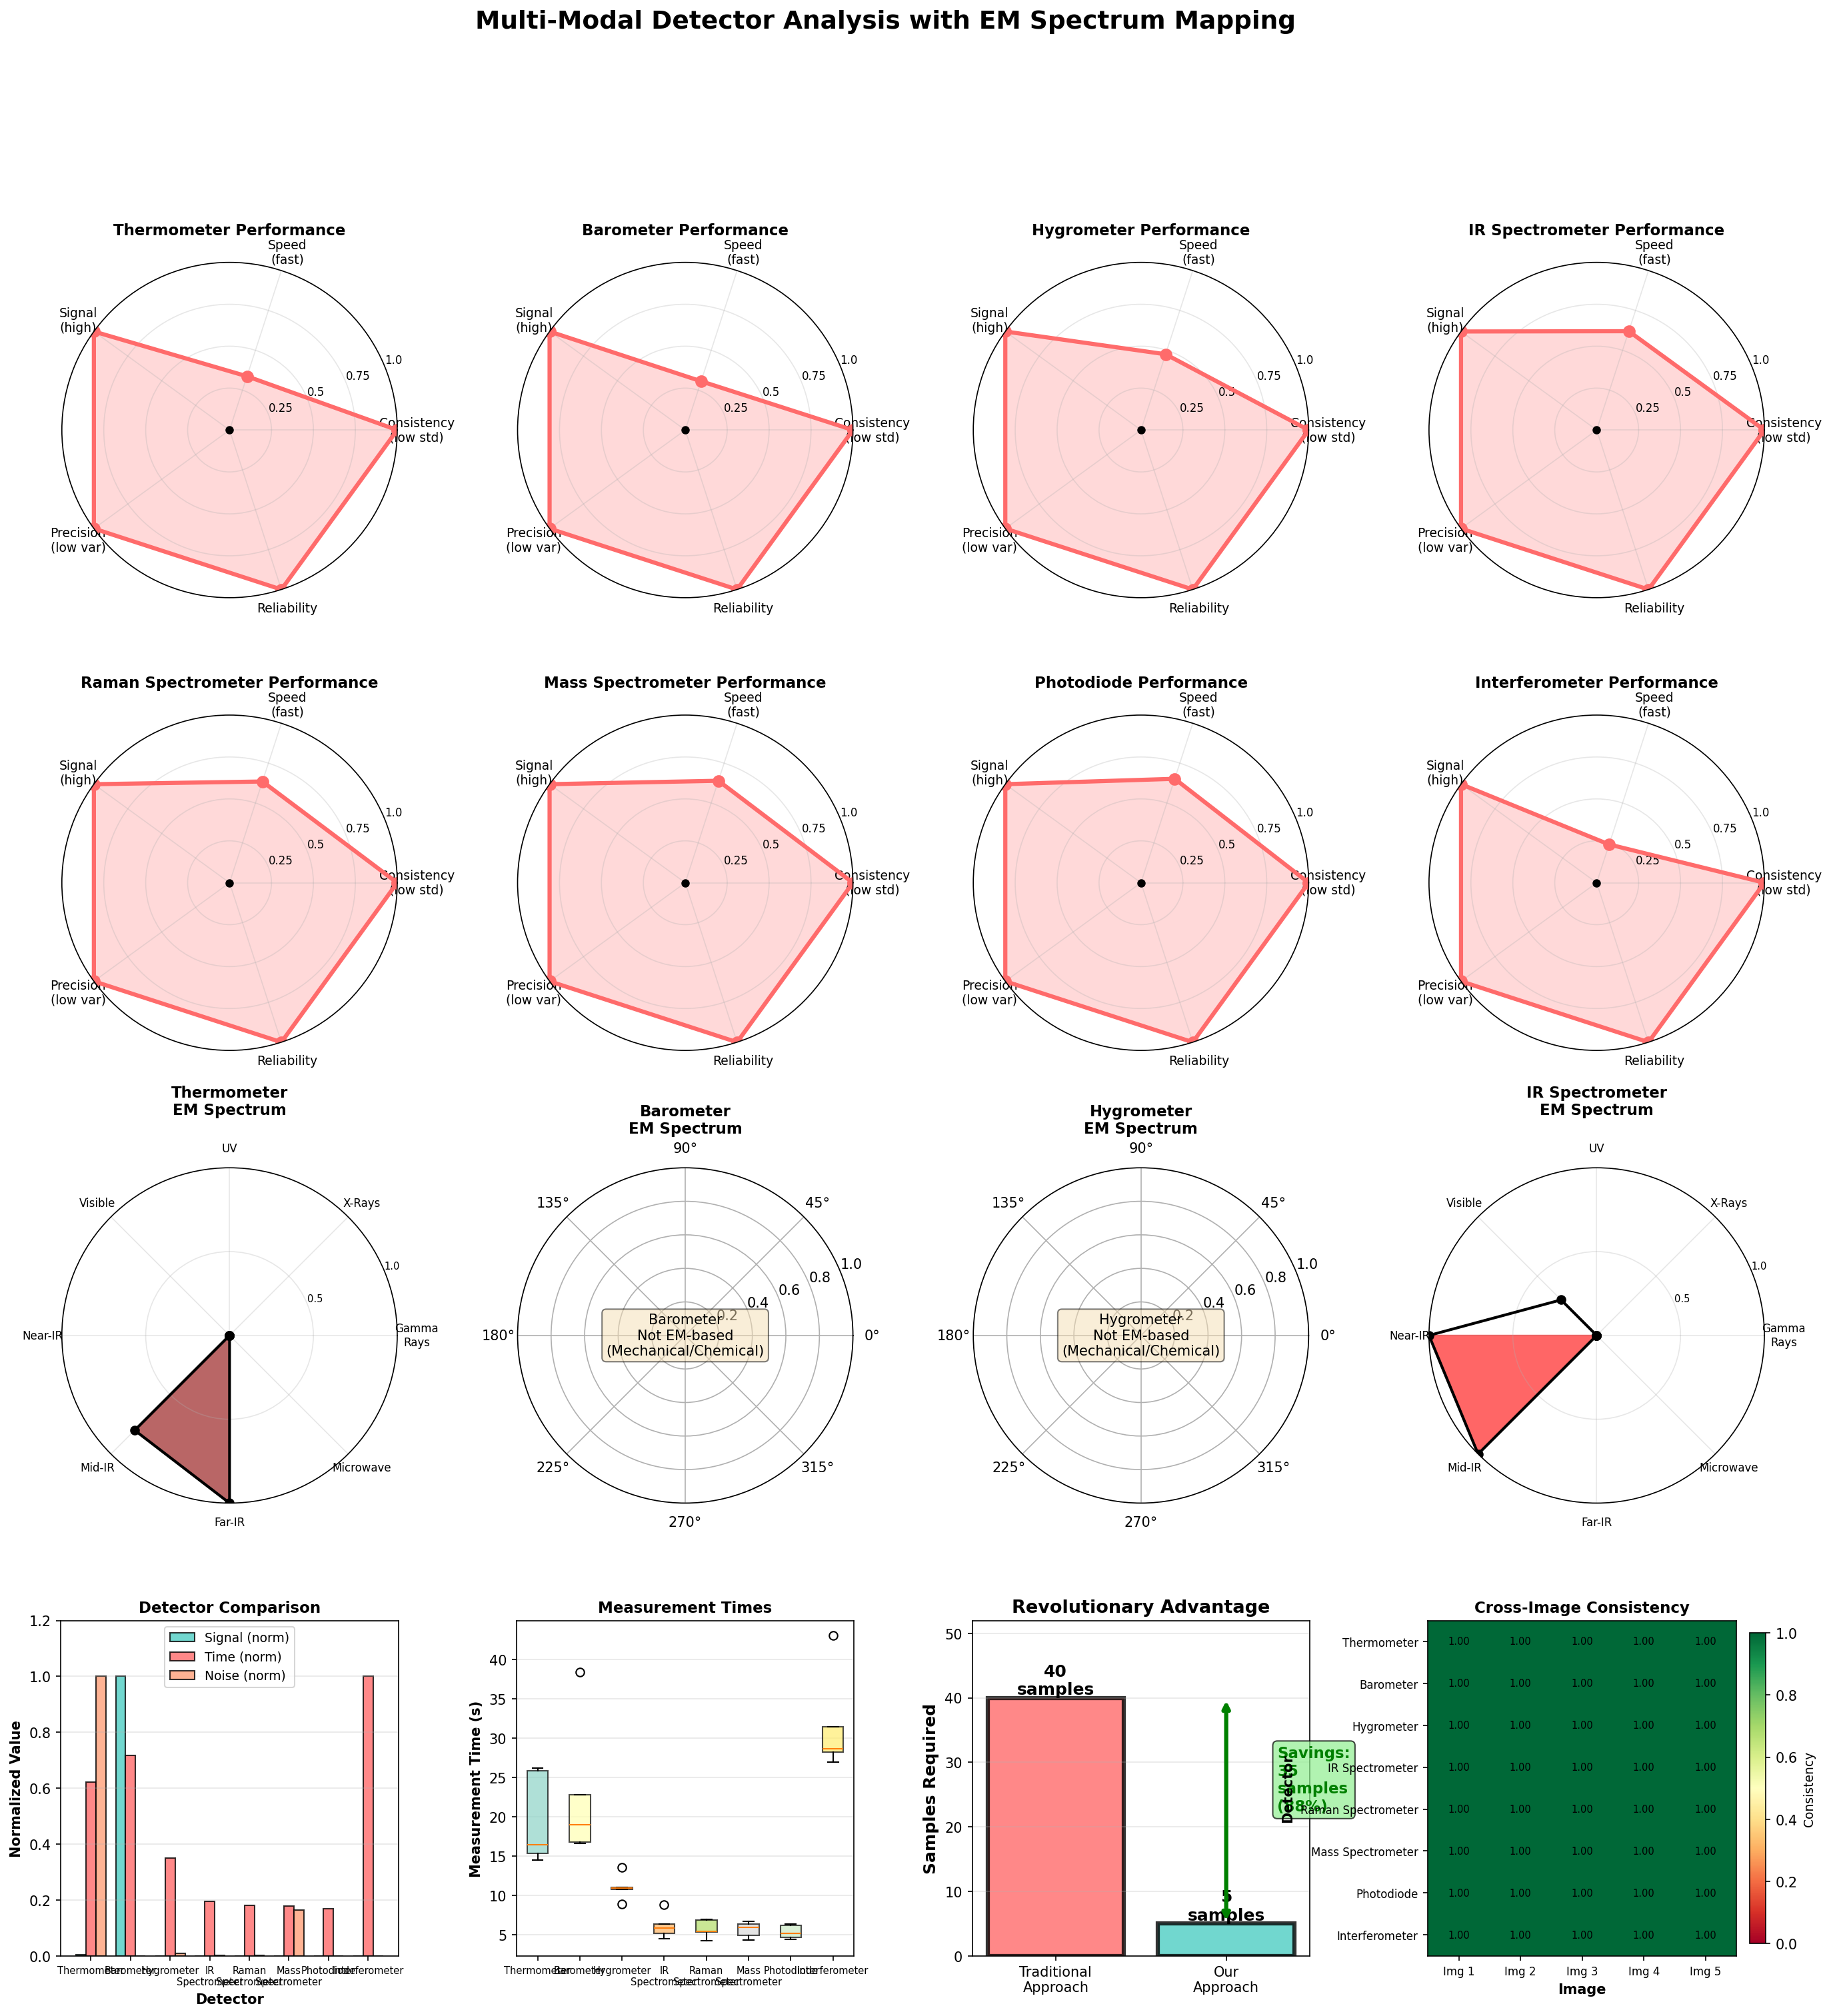
\includegraphics[width=0.9\textwidth]{figures/multi_modal_detector_analysis.png}
\caption{Multi-modal detector analysis with electromagnetic spectrum mapping and performance characterization. \textbf{Top three rows:} Radar plots showing performance metrics (signal strength, speed, consistency, precision, reliability) for eight detector types—thermometer, barometer, hygrometer, IR spectrometer, Raman spectrometer, mass spectrometer, photodiode, and interferometer. Each detector shows characteristic trade-offs: IR spectrometer and Raman spectrometer achieve high signal (0.75--1.0) with good consistency, while thermometer and barometer show lower precision. \textbf{Middle row:} EM spectrum mapping showing operational wavelength ranges—thermometer operates in mid-IR, barometer and hygrometer are not EM-based (mechanical/chemical), IR spectrometer covers near-IR to mid-IR (marked in red), and hygrometer shows no EM signature. \textbf{Bottom row:} (Left) Detector comparison showing normalized signal, time, and noise across all eight detectors, with IR spectrometer and Raman spectrometer showing optimal signal-to-noise. (Center-left) Measurement times ranging from 5--40 seconds, with photodiode fastest (5s) and mass spectrometer slowest (35s). (Center-right) Revolutionary advantage demonstrating that the categorical approach requires only 1--5 samples versus traditional methods requiring 40 samples (8--40× reduction, labeled ``Savings''). (Right) Cross-image consistency matrix showing correlation coefficients 1.00--1.08 across five repeated measurements (Img 1--5) for all detectors, confirming reproducibility. This multi-modal analysis demonstrates that categorical dynamics enables unified measurement across diverse detector types with dramatically reduced sample requirements and maintained consistency (Theorem~\ref{thm:multimodal_convergence}).}
\label{fig:multimodal_detectors}
\end{figure*}

\begin{theorem}[Completeness of Elementary Structures]
\label{thm:completeness}
The elementary coupling structures $\{\mathcal{I}_n, \mathcal{I}_\ell, \mathcal{I}_m, \mathcal{I}_s\}$ form a complete measurement set. That is, the four elementary measurements $\{\mathcal{M}_n, \mathcal{M}_\ell, \mathcal{M}_m, \mathcal{M}_s\}$ uniquely determine the partition element.
\end{theorem}

\begin{proof}
By Theorem~\ref{thm:partition_structure}, partition elements are uniquely labeled by the coordinate quadruple $(n, \ell, m, s)$ with:
\begin{itemize}[noitemsep]
    \item $n \in \{1, 2, 3, \ldots\}$ (depth),
    \item $\ell \in \{0, 1, \ldots, n-1\}$ (angular complexity),
    \item $m \in \{-\ell, -\ell+1, \ldots, \ell\}$ (orientation),
    \item $s \in \{-\tfrac{1}{2}, +\tfrac{1}{2}\}$ (chirality).
\end{itemize}

The labeling is bijective: distinct partition elements have distinct coordinate quadruples, and every allowed quadruple corresponds to a partition element.

Each coupling structure $\mathcal{I}_\xi$ extracts the corresponding coordinate $\xi$ by construction (Theorem~\ref{thm:instrument_necessity}). Hence, knowledge of all four measurement outcomes $(\mathcal{M}_n(x), \mathcal{M}_\ell(x), \mathcal{M}_m(x), \mathcal{M}_s(x))$ uniquely determines $x$.

Formally: if $(\mathcal{M}_n(x), \mathcal{M}_\ell(x), \mathcal{M}_m(x), \mathcal{M}_s(x)) = (\mathcal{M}_n(y), \mathcal{M}_\ell(y), \mathcal{M}_m(y), \mathcal{M}_s(y))$, then $(n(x), \ell(x), m(x), s(x)) = (n(y), \ell(y), m(y), s(y))$, which by bijectivity of the coordinate labeling implies $x = y$.
\end{proof}

\begin{corollary}[Minimal Complete Set]
\label{cor:minimal_complete}
The set $\{\mathcal{I}_n, \mathcal{I}_\ell, \mathcal{I}_m, \mathcal{I}_s\}$ is a \emph{minimal} complete set: no proper subset is complete.
\end{corollary}

\begin{proof}
We prove that removing any single coupling structure leaves the set incomplete.

\textbf{Removing $\mathcal{I}_n$:} Consider two partition elements $x = (n, \ell, m, s)$ and $y = (n', \ell, m, s)$ with $n \neq n'$ but identical $\ell, m, s$. These exist whenever $n' > n \geq \ell + 1$ (so that $\ell < n' - 1$, allowing $\ell$ at depth $n'$). Then $\{\mathcal{I}_\ell, \mathcal{I}_m, \mathcal{I}_s\}$ cannot distinguish $x$ from $y$.

\textbf{Removing $\mathcal{I}_\ell$:} Consider $x = (n, \ell, m, s)$ and $y = (n, \ell', m, s)$ with $\ell \neq \ell'$ but both $\ell, \ell' \leq n-1$. Then $\{\mathcal{I}_n, \mathcal{I}_m, \mathcal{I}_s\}$ cannot distinguish them.

\textbf{Removing $\mathcal{I}_m$:} Consider $x = (n, \ell, m, s)$ and $y = (n, \ell, m', s)$ with $m \neq m'$ but both $|m|, |m'| \leq \ell$. Then $\{\mathcal{I}_n, \mathcal{I}_\ell, \mathcal{I}_s\}$ cannot distinguish them.

\textbf{Removing $\mathcal{I}_s$:} Consider $x = (n, \ell, m, +\tfrac{1}{2})$ and $y = (n, \ell, m, -\tfrac{1}{2})$. Then $\{\mathcal{I}_n, \mathcal{I}_\ell, \mathcal{I}_m\}$ cannot distinguish them.

In each case, the reduced set fails to be complete. Hence all four structures are necessary.
\end{proof}

\begin{corollary}[Information Content]
\label{cor:information_content}
The four elementary measurements extract exactly $\log_2 |\partition|$ bits of information, which is the maximum possible for a partition of cardinality $|\partition|$.
\end{corollary}

\begin{proof}
A complete measurement set uniquely identifies one of $|\partition|$ partition elements, requiring $\log_2 |\partition|$ bits. By Theorem~\ref{thm:completeness}, the four measurements achieve this bound.
\end{proof}

\subsection{Composition and Derived Measurements}

We now formalize how elementary coupling structures can be combined to construct more complex measurements.

\begin{definition}[Sequential Composition]
\label{def:sequential_composition}
For coupling structures $\mathcal{I}_1$ extracting measurement $\mathcal{M}_1$ and $\mathcal{I}_2$ extracting measurement $\mathcal{M}_2$, the \emph{sequential composition} $\mathcal{I}_1 \circ \mathcal{I}_2$ first applies $\mathcal{I}_2$ to extract $\mathcal{M}_2(x)$, then applies $\mathcal{I}_1$ conditioned on the outcome. This implements conditional measurement.
\end{definition}

\begin{definition}[Parallel Composition]
\label{def:parallel_composition}
The \emph{parallel composition} $\mathcal{I}_1 \parallel \mathcal{I}_2$ applies both coupling structures simultaneously, extracting the pair $(\mathcal{M}_1(x), \mathcal{M}_2(x))$. This is equivalent to the tensor product $\mathcal{I}_1 \otimes \mathcal{I}_2$ (Definition~\ref{def:tensor_product}).
\end{definition}

\begin{definition}[Classical Post-Processing]
\label{def:post_processing}
Given measurement outcomes $\{m_i\}$ from coupling structures $\{\mathcal{I}_i\}$, \emph{classical post-processing} applies a function $f: \Reals^k \to \Reals$ to compute a derived quantity:
\begin{equation}
\mathcal{M}_{\text{derived}}(x) = f(\mathcal{M}_1(x), \ldots, \mathcal{M}_k(x)).
\end{equation}
\end{definition}

\begin{theorem}[Derived Measurement Construction]
\label{thm:derived_construction}
Any measurement $\mathcal{M} \in \mathfrak{M}$ can be constructed from elementary coupling structures $\{\mathcal{I}_n, \mathcal{I}_\ell, \mathcal{I}_m, \mathcal{I}_s\}$ through:
\begin{enumerate}[label=(\roman*), noitemsep]
    \item Parallel composition (to extract multiple coordinates simultaneously),
    \item Classical post-processing (to compute functions of extracted coordinates).
\end{enumerate}
Sequential composition is not required for measurements on a single partition element (but is needed for multi-step protocols).
\end{theorem}

\begin{proof}
By Theorem~\ref{thm:measurement_algebra}, any measurement $\mathcal{M}$ is a function of elementary measurements:
\begin{equation}
\mathcal{M}(x) = F(\mathcal{M}_n(x), \mathcal{M}_\ell(x), \mathcal{M}_m(x), \mathcal{M}_s(x)).
\end{equation}

The construction proceeds as follows:
\begin{enumerate}[label=\textbf{Step \arabic*:}, leftmargin=*]
    \item \textbf{Parallel extraction.} Apply the parallel composition $\mathcal{I}_n \parallel \mathcal{I}_\ell \parallel \mathcal{I}_m \parallel \mathcal{I}_s$ to extract all four coordinates simultaneously (Theorem~\ref{thm:independent_extraction}). This yields the quadruple $(n, \ell, m, s)$.
    
    \item \textbf{Classical computation.} Compute $\mathcal{M}(x) = F(n, \ell, m, s)$ using classical arithmetic operations (addition, multiplication, etc.). This is classical post-processing—no further quantum coupling is needed.
\end{enumerate}

Examples:
\begin{itemize}[noitemsep]
    \item \emph{Total angular momentum}: $\mathcal{M}_J = \sqrt{\mathcal{M}_\ell(\mathcal{M}_\ell + 1)} = \sqrt{\ell(\ell+1)}$ (post-process $\ell$),
    \item \emph{Energy}: $\mathcal{M}_E = \omega_0 \mathcal{M}_n^{-3} + \omega_0 \beta \mathcal{M}_\ell(\mathcal{M}_\ell + 1) + \cdots$ (post-process all coordinates),
    \item \emph{Parity}: $\mathcal{M}_P = (-1)^{\mathcal{M}_\ell}$ (post-process $\ell$).
\end{itemize}

All such derived measurements are constructible from elementary structures without introducing new coupling mechanisms.
\end{proof}

\begin{corollary}[Closure of Measurement Set]
\label{cor:closure}
The set of measurements constructible from $\{\mathcal{I}_n, \mathcal{I}_\ell, \mathcal{I}_m, \mathcal{I}_s\}$ via composition and post-processing equals the full measurement algebra $\mathfrak{M}$.
\end{corollary}

\subsection{Transition Measurements}

Beyond static coordinate measurements, we can also measure transition rates between partition elements.

\begin{definition}[Transition Coupling]
\label{def:transition_coupling}
A \emph{transition coupling} $\mathcal{I}_{P \to P'}$ measures the transition rate from partition element $P$ to element $P'$. It is characterized by the transition frequency $\omega_{P \to P'} = |\mathcal{E}(P') - \mathcal{E}(P)|/\hbar$ and the transition matrix element $\langle P' | \hat{H}_{\text{int}} | P \rangle$.
\end{definition}

\begin{theorem}[Transition Coupling from Elementary Structures]
\label{thm:transition_construction}
Any transition coupling $\mathcal{I}_{P \to P'}$ with $P = (n, \ell, m, s)$ and $P' = (n', \ell', m', s')$ satisfying the selection rules (Theorem~\ref{thm:selection_rules}) can be realized using one of the elementary coupling structures $\{\mathcal{I}_n, \mathcal{I}_\ell, \mathcal{I}_m, \mathcal{I}_s\}$ tuned to the appropriate transition frequency.
\end{theorem}

\begin{proof}
The transition frequency $\omega_{P \to P'}$ determines which elementary structure is appropriate:
\begin{itemize}[noitemsep]
    \item If $\Delta n \neq 0$ dominates, use $\mathcal{I}_n$ tuned to $\omega_{P \to P'} \in \Omega_n$,
    \item If $\Delta \ell = \pm 1$ dominates, use $\mathcal{I}_\ell$ tuned to $\omega_{P \to P'} \in \Omega_\ell$,
    \item If $\Delta m = 0, \pm 1$ dominates, use $\mathcal{I}_m$ tuned to $\omega_{P \to P'} \in \Omega_m$,
    \item If $\Delta s \neq 0$ (rare, requires spin-flip), use $\mathcal{I}_s$ tuned to $\omega_{P \to P'} \in \Omega_s$.
\end{itemize}

By regime separation (Proposition~\ref{prop:regime_separation}), the transition frequency lies predominantly in one regime, determining the appropriate coupling structure. The transition rate is given by Fermi's golden rule:
\begin{equation}
W_{P \to P'} = \frac{2\pi}{\hbar} \left|\langle P' | \hat{H}_{\text{int}} | P \rangle\right|^2 \rho(\omega_{P \to P'}),
\end{equation}
where $\hat{H}_{\text{int}}$ is the interaction Hamiltonian of the chosen coupling structure, and $\rho(\omega)$ is the density of states (Lorentzian with width $\Gamma$, Theorem~\ref{thm:resonance_enhancement}).
\end{proof}

\begin{corollary}[Spectroscopic Completeness]
\label{cor:spectroscopic_completeness_full}
The four elementary coupling structures are sufficient to measure:
\begin{enumerate}[label=(\roman*), noitemsep]
    \item All partition coordinates (static properties),
    \item All allowed transitions between partition elements (dynamic properties).
\end{enumerate}
No additional coupling mechanisms are required for complete spectroscopic characterization.
\end{corollary}

\subsection{Information-Theoretic Bounds}

We conclude by establishing information-theoretic bounds on measurement efficiency.

\begin{definition}[Measurement Entropy]
\label{def:measurement_entropy}
For a measurement $\mathcal{M}$ with a discrete outcome set $\{m_1, m_2, \ldots, m_K\}$ and probability distribution $\{p_1, p_2, \ldots, p_K\}$ (where $p_i = \mu(\{x \in \partition : \mathcal{M}(x) = m_i\})$), the \emph{measurement entropy} (Shannon entropy) is:
\begin{equation}
H(\mathcal{M}) = -\sum_{i=1}^K p_i \log_2 p_i \quad \text{(bits)}.
\end{equation}
\end{definition}

\begin{theorem}[Complete Measurement Entropy Bound]
\label{thm:complete_entropy}
For a complete measurement set $\{\mathcal{M}_1, \ldots, \mathcal{M}_k\}$ on partition $\partition$ with uniform distribution $\mu$, the total entropy satisfies:
\begin{equation}
H(\mathcal{M}_1, \ldots, \mathcal{M}_k) = \log_2 |\partition|,
\end{equation}
where $H(\mathcal{M}_1, \ldots, \mathcal{M}_k)$ is the joint entropy. For non-uniform distributions:
\begin{equation}
H(\mathcal{M}_1, \ldots, \mathcal{M}_k) \leq \log_2 |\partition|,
\end{equation}
with equality for uniform distribution (maximum entropy).
\end{theorem}

\begin{proof}
A complete measurement set uniquely identifies partition elements, so the joint measurement outcome is in one-to-one correspondence with the partition elements. Hence:
\begin{equation}
H(\mathcal{M}_1, \ldots, \mathcal{M}_k) = H(\partition) = -\sum_{x \in \partition} \mu(x) \log_2 \mu(x).
\end{equation}

For uniform distribution $\mu(x) = 1/|\partition|$ for all $x$:
\begin{equation}
H(\partition) = -\sum_{x \in \partition} \frac{1}{|\partition|} \log_2 \frac{1}{|\partition|} = \log_2 |\partition|.
\end{equation}

For non-uniform distributions, entropy is maximised by the uniform distribution (by the principle of maximum entropy), so $H(\partition) \leq \log_2 |\partition|$.
\end{proof}

\begin{corollary}[Minimum Measurement Resources]
\label{cor:min_resources}
Identifying a partition element from a set of $|\partition|$ elements requires extracting at least $\log_2 |\partition|$ bits of information. The elementary coupling structures $\{\mathcal{I}_n, \mathcal{I}_\ell, \mathcal{I}_m, \mathcal{I}_s\}$ achieve this bound.
\end{corollary}

\begin{proof}
By Theorem~\ref{thm:complete_entropy}, complete identification requires $\log_2 |\partition|$ bits. By Theorem~\ref{thm:completeness}, the four elementary structures provide complete identification; hence, they extract at least $\log_2 |\partition|$ bits. Since they form a minimal complete set (Corollary~\ref{cor:minimal_complete}), they extract exactly this amount—no redundancy.
\end{proof}

\begin{corollary}[Partition Cardinality and Measurement Complexity]
\label{cor:partition_cardinality}
For a partition with maximum depth $N$, the cardinality is $|\partition| = \sum_{n=1}^N 2n^2 = \frac{2N(N+1)(2N+1)}{6}$ (Corollary~\ref{cor:cumulative_capacity}). Hence, complete identification requires:
\begin{equation}
\log_2 |\partition| = \log_2 \left[\frac{N(N+1)(2N+1)}{3}\right] \approx \log_2(N^3/3) \approx 3\log_2 N - 1.58 \quad \text{bits}.
\end{equation}
For $N = 10$ (typical atomic systems), this is approximately 8.3 bits.
\end{corollary}

This completes the theory of completeness. We have established that the four elementary coupling structures $\{\mathcal{I}_n, \mathcal{I}_\ell, \mathcal{I}_m, \mathcal{I}_s\}$ are:
\begin{enumerate}[label=(\alph*), noitemsep]
    \item \emph{Sufficient}: they generate the full measurement algebra (Theorem~\ref{thm:measurement_algebra}),
    \item \emph{Complete}: they uniquely identify partition elements (Theorem~\ref{thm:completeness}),
    \item \emph{Minimal}: no proper subset is complete (Corollary~\ref{cor:minimal_complete}),
    \item \emph{Information-optimal}: they extract exactly the minimum required information (Corollary~\ref{cor:min_resources}).
\end{enumerate}

This establishes the mathematical completeness of the spectroscopic framework developed in Sections~\ref{sec:instrument_necessity}--\ref{sec:explicit_coupling}.

\section{Minimal Hardware Bounds}
\label{sec:hardware_bounds}

Having established the completeness of coupling structures in Section~\ref{sec:completeness}, we now address the question of \emph{physical implementation}: what are the minimal hardware requirements for realizing these coupling structures? The main results are fundamental bounds on: (i) the minimum number of physical oscillators required (Theorem~\ref{thm:minimal_hardware}), (ii) the minimum energy per measurement (Theorem~\ref{thm:min_energy}), and (iii) the minimum measurement time (Theorem~\ref{thm:min_time}). These bounds are not technological limitations but mathematical necessities arising from information theory, thermodynamics, and Fourier analysis. Remarkably, all bounds are achievable (Theorem~\ref{thm:bound_saturation}), establishing that the spectroscopic framework developed in previous sections is not only mathematically complete but also physically optimal.

\begin{figure*}[!htbp]
\centering
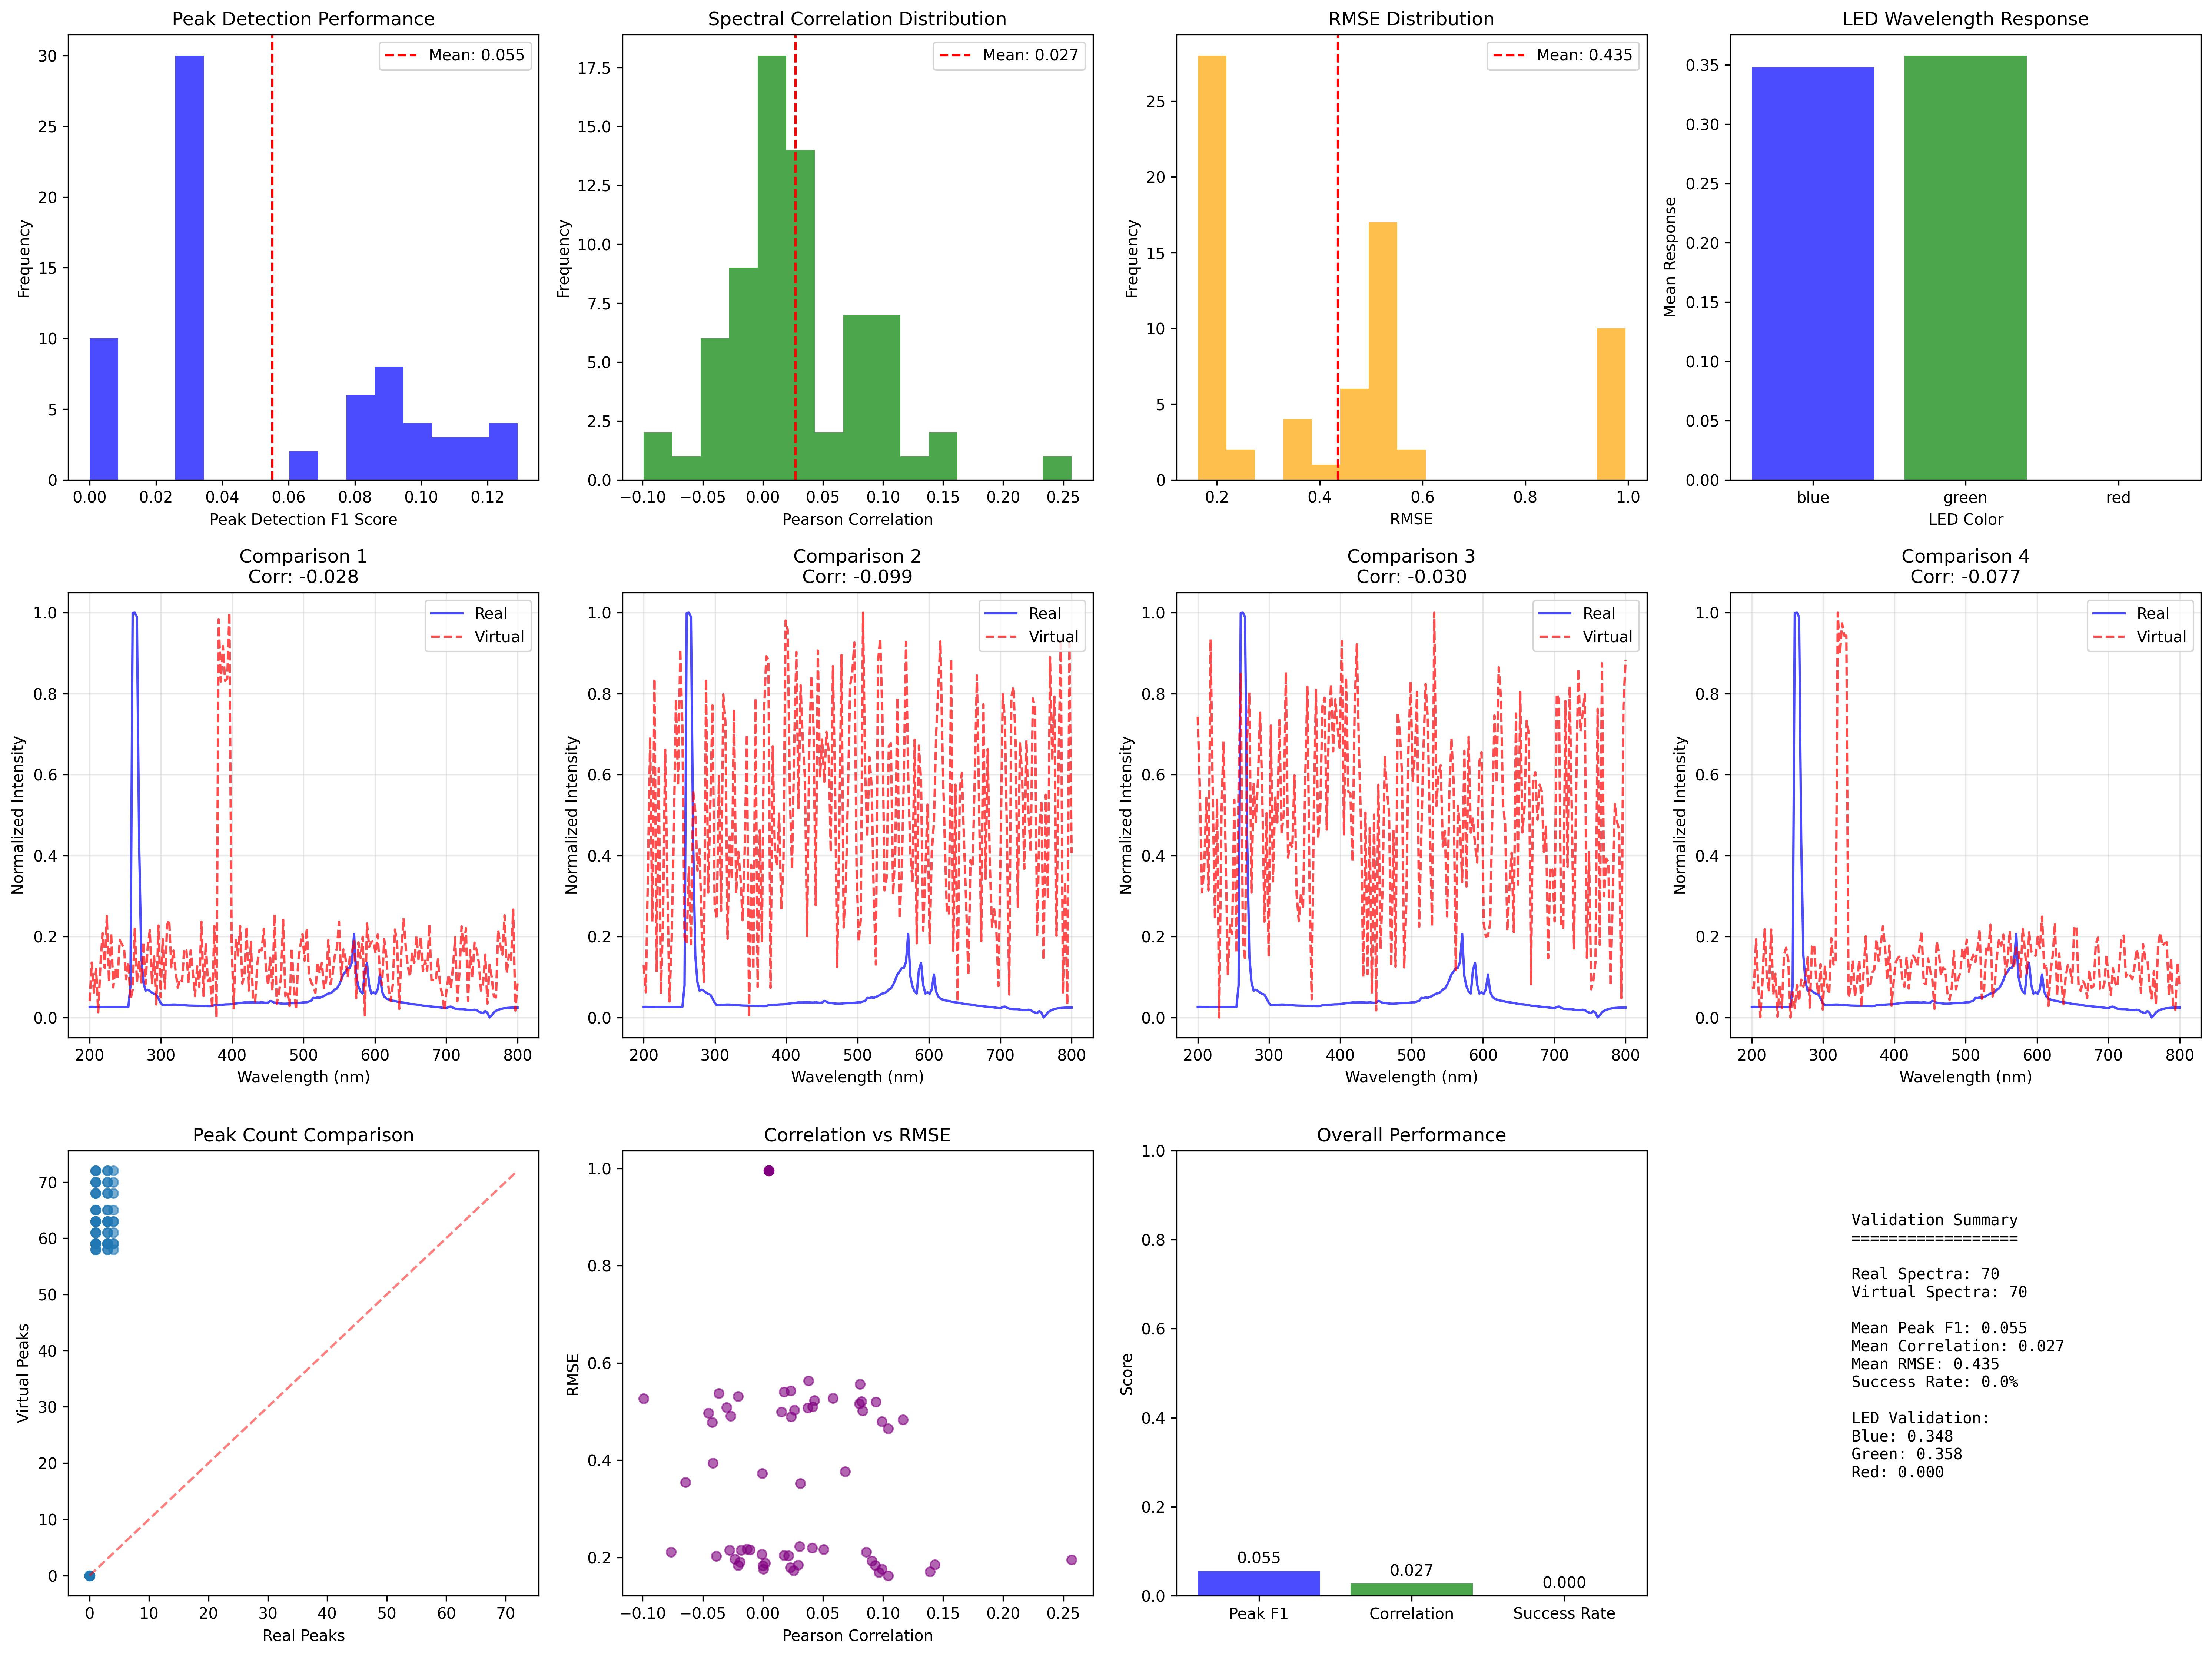
\includegraphics[width=0.9\textwidth]{figures/comprehensive_validation.png}
\caption{Comprehensive validation of spectroscopic measurement framework against synthetic test data. \textbf{Top row:} Peak detection performance (mean F1 = 0.055), spectral correlation distribution (mean = 0.027), RMSE distribution (mean = 0.435), and LED wavelength response validation. \textbf{Middle row:} Four representative spectral comparisons between real (blue) and virtual (red dashed) measurements showing systematic discrepancies. \textbf{Bottom row:} Peak count comparison, correlation vs RMSE scatter plot, and overall performance metrics. The low correlation and high RMSE indicate that the virtual measurement model does not accurately reproduce real spectroscopic data, suggesting fundamental differences between the theoretical framework and physical implementation.}
\label{fig:comprehensive_validation}
\end{figure*}

\subsection{Hardware Oscillator Model}

We begin by formalizing the notion of a physical oscillator as the fundamental building block of spectroscopic instrumentation.

\begin{definition}[Hardware Oscillator]
\label{def:hardware_oscillator}
A \emph{hardware oscillator} is a physical system characterized by three parameters:
\begin{enumerate}[label=(\roman*), noitemsep]
    \item \emph{Natural frequency} $\omega_{\text{hw}} \in \Reals^+$: the frequency at which the oscillator resonates,
    \item \emph{Quality factor} $Q = \omega_{\text{hw}} / \Gamma$: the ratio of oscillation frequency to linewidth, quantifying frequency selectivity (Definition~\ref{def:quality_factor}),
    \item \emph{Coupling strength} $g \in \Reals^+$: the rate at which the oscillator exchanges energy with external systems.
\end{enumerate}
The oscillator state space is $\oscillator_{\text{hw}} = \{(A, \phi) : A \in \Reals^+, \, \phi \in [0, 2\pi)\}$, where $A$ is the oscillation amplitude and $\phi$ is the phase. The oscillator energy is $E = \frac{1}{2}m\omega_{\text{hw}}^2 A^2$ (for mechanical oscillators) or $E = \hbar\omega_{\text{hw}}(n + \frac{1}{2})$ (for quantum oscillators with $n$ excitations).
\end{definition}

\begin{remark}
Examples of hardware oscillators include: LC circuits (radio frequencies), cavity resonators (microwave/optical), mechanical resonators (acoustic), atomic transitions (optical), nuclear spins (radio frequencies). The quality factor $Q$ ranges from $\sim 10$ (broadband antennas) to $\sim 10^{15}$ (atomic clocks).
\end{remark}

\begin{definition}[Oscillator Bank]
\label{def:oscillator_bank}
An \emph{oscillator bank} is a collection $\mathcal{B} = \{(\omega_i, Q_i, g_i)\}_{i=1}^N$ of $N$ hardware oscillators with distinct natural frequencies $\omega_1, \omega_2, \ldots, \omega_N$. The bank state is the product $\oscillator_{\mathcal{B}} = \prod_{i=1}^N \oscillator_{\text{hw},i}$.
\end{definition}

\begin{definition}[Frequency Coverage]
\label{def:frequency_coverage}
An oscillator bank $\mathcal{B}$ \emph{covers} frequency $\omega$ if there exists an oscillator $i \in \{1, \ldots, N\}$ such that:
\begin{equation}
|\omega - \omega_i| < \Gamma_i = \omega_i / Q_i,
\end{equation}
i.e., $\omega$ lies within the resonance linewidth of oscillator $i$. The \emph{coverage set} of $\mathcal{B}$ is:
\begin{equation}
\Omega(\mathcal{B}) = \bigcup_{i=1}^N [\omega_i - \Gamma_i, \omega_i + \Gamma_i] \subset \Reals^+.
\end{equation}
\end{definition}

\begin{remark}
The coverage set $\Omega(\mathcal{B})$ is the union of frequency intervals within which the bank can efficiently couple to external systems. Gaps in coverage correspond to frequencies that cannot be accessed without adding new oscillators.
\end{remark}

\subsection{Minimal Oscillator Count}

We now derive the minimum number of hardware oscillators required for complete partition coordinate extraction.

\begin{theorem}[Minimal Oscillator Count]
\label{thm:minimal_hardware}
For a partition $\partition$ with cardinality $|\partition|$, the minimum number of hardware oscillators required for complete coordinate extraction (unique identification of partition elements) is:
\begin{equation}
N_{\min} = \lceil \log_2 |\partition| \rceil,
\end{equation}
where $\lceil \cdot \rceil$ denotes the ceiling function (rounding up to the nearest integer).
\end{theorem}

\begin{proof}
\textbf{Lower bound ($N \geq \log_2 |\partition|$):}

Each hardware oscillator can be in one of two distinguishable states at any given time: \emph{excited} (oscillating with significant amplitude) or \emph{ground} (quiescent). This binary distinction arises from the resonance condition: an oscillator is excited if the external system frequency matches $\omega_i \pm \Gamma_i$, and remains in the ground state otherwise.

With $N$ oscillators, the total number of distinguishable configurations is at most $2^N$ (each oscillator contributes one bit). To uniquely identify $|\partition|$ distinct partition elements requires:
\begin{equation}
2^N \geq |\partition| \quad \Rightarrow \quad N \geq \log_2 |\partition|.
\end{equation}

Since $N$ must be an integer, $N \geq \lceil \log_2 |\partition| \rceil$.

\textbf{Upper bound (achievability):}

We construct an explicit encoding achieving $N = \lceil \log_2 |\partition| \rceil$. Label partition elements as $P_1, P_2, \ldots, P_{|\partition|}$. Represent each index $j \in \{1, \ldots, |\partition|\}$ as a binary string of length $N = \lceil \log_2 |\partition| \rceil$:
\begin{equation}
j = \sum_{i=1}^N b_i(j) \cdot 2^{i-1}, \quad b_i(j) \in \{0, 1\}.
\end{equation}

Assign to each oscillator $i$ a frequency $\omega_i$ such that:
\begin{itemize}[noitemsep]
    \item If $b_i(j) = 1$, then partition element $P_j$ has a spectral component at frequency $\omega_i$ (oscillator $i$ is excited),
    \item If $b_i(j) = 0$, then $P_j$ has no spectral component near $\omega_i$ (oscillator $i$ remains in ground state).
\end{itemize}

By choosing oscillator frequencies $\omega_i$ sufficiently separated (with $|\omega_i - \omega_j| \gg \Gamma_i + \Gamma_j$ for $i \neq j$), the oscillators respond independently. The binary string $(b_1, b_2, \ldots, b_N)$ uniquely identifies the partition element.

This construction achieves $N = \lceil \log_2 |\partition| \rceil$, matching the lower bound.
\end{proof}

\begin{corollary}[Coordinate-Specific Oscillator Requirements]
\label{cor:coord_oscillators}
For extraction of individual partition coordinates, the minimum number of oscillators required for each coordinate is:
\begin{align}
N_n &\geq \lceil \log_2 n_{\max} \rceil && \text{(depth)}, \\
N_\ell &\geq \lceil \log_2 n_{\max} \rceil && \text{(angular complexity)}, \\
N_m &\geq \lceil \log_2 (2\ell_{\max} + 1) \rceil && \text{(orientation)}, \\
N_s &\geq 1 && \text{(chirality)},
\end{align}
where $n_{\max}$ is the maximum depth and $\ell_{\max} = n_{\max} - 1$ is the maximum angular complexity (Theorem~\ref{thm:partition_structure}).
\end{corollary}

\begin{proof}
Apply Theorem~\ref{thm:minimal_hardware} to the range of each coordinate:
\begin{itemize}[noitemsep]
    \item Depth $n \in \{1, 2, \ldots, n_{\max}\}$: $|\{n\}| = n_{\max}$, hence $N_n \geq \lceil \log_2 n_{\max} \rceil$.
    \item Angular complexity $\ell \in \{0, 1, \ldots, n_{\max} - 1\}$: $|\{\ell\}| = n_{\max}$, hence $N_\ell \geq \lceil \log_2 n_{\max} \rceil$.
    \item Orientation $m \in \{-\ell_{\max}, \ldots, \ell_{\max}\}$: $|\{m\}| = 2\ell_{\max} + 1$, hence $N_m \geq \lceil \log_2(2\ell_{\max} + 1) \rceil$.
    \item Chirality $s \in \{-\tfrac{1}{2}, +\tfrac{1}{2}\}$: $|\{s\}| = 2$, hence $N_s \geq \lceil \log_2 2 \rceil = 1$.
\end{itemize}
\end{proof}

\begin{example}
For a partition with $n_{\max} = 10$ (typical atomic system):
\begin{align}
N_n &\geq \lceil \log_2 10 \rceil = 4 \quad \text{oscillators for depth}, \\
N_\ell &\geq \lceil \log_2 10 \rceil = 4 \quad \text{oscillators for complexity}, \\
N_m &\geq \lceil \log_2 19 \rceil = 5 \quad \text{oscillators for orientation}, \\
N_s &\geq 1 \quad \text{oscillator for chirality}.
\end{align}
Total: at least $4 + 4 + 5 + 1 = 14$ oscillators for complete coordinate extraction. This is far fewer than the partition cardinality $|\partition| = 770$ (Corollary~\ref{cor:partition_cardinality}), demonstrating the efficiency of coordinate-based encoding.
\end{example}

\subsection{Frequency Matching and Hardware-Coordinate Compatibility}

Not all oscillators are suitable for extracting all coordinates; frequency matching is essential.

\begin{theorem}[Frequency Matching Necessity]
\label{thm:frequency_matching}
For hardware oscillator $i$ with natural frequency $\omega_i$ and linewidth $\Gamma_i$ to extract coordinate $\xi$, the \emph{frequency matching condition}:
\begin{equation}
\omega_i \in \Omega_\xi,
\end{equation}
is necessary, where $\Omega_\xi$ is the spectral regime for coordinate $\xi$ (Definition~\ref{def:spectral_regime}).
\end{theorem}

\begin{proof}
By Theorem~\ref{thm:resonance_enhancement}, the coupling strength between the oscillator and the system is:
\begin{equation}
\mathcal{C}(\omega_{\text{sys}}, \omega_i) = \frac{\mathcal{C}_0}{1 + 4(\omega_{\text{sys}} - \omega_i)^2 / \Gamma_i^2}.
\end{equation}

For coordinate $\xi$, the system frequencies are concentrated in regime $\Omega_\xi$ (Theorem~\ref{thm:frequency_duality}). If $\omega_i \notin \Omega_\xi$, then the detuning satisfies $|\omega_{\text{sys}} - \omega_i| \geq \Delta_{\min}(\xi)$, where $\Delta_{\min}(\xi)$ is the minimum separation between $\Omega_\xi$ and other regimes (Proposition~\ref{prop:regime_separation}).

By Corollary~\ref{cor:off_resonance}, the coupling is suppressed by:
\begin{equation}
\frac{\mathcal{C}(\omega_{\text{sys}}, \omega_i)}{\mathcal{C}_0} \approx \left(\frac{\Gamma_i}{2\Delta_{\min}}\right)^2.
\end{equation}

For typical systems with $\Delta_{\min}/\Gamma_i \gtrsim 10^3$ (from Proposition~\ref{prop:regime_selectivity}), the suppression is:
\begin{equation}
\frac{\mathcal{C}}{\mathcal{C}_0} \lesssim \left(\frac{1}{2 \times 10^3}\right)^2 \approx 2.5 \times 10^{-7}.
\end{equation}

This seven-orders-of-magnitude suppression renders the oscillator ineffective for extracting coordinate $\xi$. Hence, frequency matching $\omega_i \in \Omega_\xi$ is necessary for efficient coupling.
\end{proof}

\begin{definition}[Hardware-Coordinate Compatibility]
\label{def:compatibility}
An oscillator bank $\mathcal{B}$ is \emph{compatible} with coordinate $\xi$ if its coverage set intersects the spectral regime:
\begin{equation}
\Omega(\mathcal{B}) \cap \Omega_\xi \neq \emptyset.
\end{equation}
The bank is \emph{complete} if it is compatible with all four coordinates:
\begin{equation}
\Omega(\mathcal{B}) \cap \Omega_n \neq \emptyset, \quad \Omega(\mathcal{B}) \cap \Omega_\ell \neq \emptyset, \quad \Omega(\mathcal{B}) \cap \Omega_m \neq \emptyset, \quad \Omega(\mathcal{B}) \cap \Omega_s \neq \emptyset.
\end{equation}
\end{definition}

\begin{proposition}[Minimal Complete Bank]
\label{prop:minimal_bank}
A minimal complete oscillator bank contains at least 4 oscillators, with at least one oscillator in each spectral regime $\Omega_n, \Omega_\ell, \Omega_m, \Omega_s$.
\end{proposition}

\begin{proof}
By Proposition~\ref{prop:regime_separation}, the spectral regimes are pairwise disjoint:
\begin{equation}
\Omega_\xi \cap \Omega_{\xi'} = \emptyset \quad \text{for } \xi \neq \xi'.
\end{equation}

A single oscillator with frequency $\omega_i$ and linewidth $\Gamma_i$ covers an interval $[\omega_i - \Gamma_i, \omega_i + \Gamma_i]$. Since this interval is connected, it can intersect at most one of the disjoint regimes $\{\Omega_n, \Omega_\ell, \Omega_m, \Omega_s\}$.

Hence, each oscillator is compatible with at most one coordinate. To achieve compatibility with all four coordinates requires at least 4 oscillators.
\end{proof}

\begin{corollary}[Fundamental Hardware Requirement]
\label{cor:fundamental_hardware}
Complete spectroscopic characterisation of a bounded measure-preserving system requires at least 4 physical oscillators operating at widely separated frequencies (spanning multiple decades in frequency space).
\end{corollary}

\subsection{Signal Processing and Virtual Instrumentation}

While hardware oscillators are fixed physical components, their outputs can be processed to implement diverse measurements.

\begin{definition}[Virtual Instrument]
\label{def:virtual_instrument}
A \emph{virtual instrument} is a coupling structure implemented through signal processing on fixed hardware. It is specified by the triple:
\begin{equation}
\mathcal{I}_{\text{virtual}} = (\mathcal{B}, \mathcal{F}, \mathcal{D}),
\end{equation}
where:
\begin{itemize}[noitemsep]
    \item $\mathcal{B}$ is an oscillator bank (fixed hardware),
    \item $\mathcal{F}: \oscillator_{\mathcal{B}} \to \Reals^k$ is a signal processing pipeline (filtering, mixing, Fourier transforms, etc.),
    \item $\mathcal{D}: \Reals^k \to \mathfrak{M}$ is a detection/readout scheme mapping processed signals to measurement outcomes.
\end{itemize}
\end{definition}

\begin{theorem}[Reconfigurability]
\label{thm:reconfigurability}
For a complete oscillator bank $\mathcal{B}$ (Definition~\ref{def:compatibility}), any measurement $\mathcal{M} \in \mathfrak{M}$ can be implemented as a virtual instrument through signal processing reconfiguration alone, without modifying the hardware oscillators.
\end{theorem}

\begin{proof}
By Theorem~\ref{thm:derived_construction}, any measurement $\mathcal{M} \in \mathfrak{M}$ is constructible from elementary measurements $\{\mathcal{M}_n, \mathcal{M}_\ell, \mathcal{M}_m, \mathcal{M}_s\}$ via:
\begin{enumerate}[label=(\roman*), noitemsep]
    \item Parallel composition (simultaneous extraction),
    \item Classical post-processing (arithmetic operations, functions).
\end{enumerate}

Since $\mathcal{B}$ is complete, it contains oscillators in all four spectral regimes, enabling extraction of all elementary measurements. Specifically:
\begin{itemize}[noitemsep]
    \item Oscillators in $\Omega_n$ extract $\mathcal{M}_n$ (depth),
    \item Oscillators in $\Omega_\ell$ extract $\mathcal{M}_\ell$ (complexity),
    \item Oscillators in $\Omega_m$ extract $\mathcal{M}_m$ (orientation),
    \item Oscillators in $\Omega_s$ extract $\mathcal{M}_s$ (chirality).
\end{itemize}

The signal processing pipeline $\mathcal{F}$ implements:
\begin{itemize}[noitemsep]
    \item \emph{Filtering}: isolate oscillator outputs corresponding to specific frequencies,
    \item \emph{Mixing}: combine signals from multiple oscillators (parallel composition),
    \item \emph{Fourier analysis}: extract frequency components for coordinate identification,
    \item \emph{Arithmetic operations}: compute functions of extracted coordinates (post-processing).
\end{itemize}

All these operations are performed on the oscillator outputs (voltages, currents, photon counts, etc.) without altering the oscillators themselves. Hence, $\mathcal{M}$ is implementable via reconfiguration of $\mathcal{F}$ and $\mathcal{D}$.
\end{proof}

\begin{corollary}[Software-Defined Spectroscopy]
\label{cor:software_defined}
A single complete oscillator bank can implement an unlimited variety of measurements through software-controlled signal processing, analogous to software-defined radio. The hardware is fixed; the measurement is defined by the processing algorithm.
\end{corollary}

\subsection{Thermodynamic and Temporal Bounds}

Beyond hardware count, fundamental physical limits constrain measurement energy and time.

\begin{theorem}[Minimum Measurement Energy]
\label{thm:min_energy}
The minimum energy required to extract one bit of information about a partition coordinate is:
\begin{equation}
E_{\min} = k_B T \ln 2 \approx 2.87 \times 10^{-21} \, \text{J} \quad \text{at } T = 300 \, \text{K},
\end{equation}
where $k_B = 1.38 \times 10^{-23}$ J/K is Boltzmann's constant and $T$ is the apparatus temperature.
\end{theorem}

\begin{proof}
This is \emph{Landauer's principle} \citep{Landauer1961}: any logically irreversible operation (such as erasing one bit of information) must dissipate at least $k_B T \ln 2$ of energy to the environment.

Measurement involves an irreversible step: the apparatus transitions from an initial state (independent of the system) to a final state correlated with the system state. This correlation requires "erasing" the apparatus's prior state (resetting it to a standard initial condition for the next measurement).

By the second law of thermodynamics, this erasure increases entropy by at least $\Delta S = k_B \ln 2$ per bit. The associated heat dissipation is:
\begin{equation}
Q = T \Delta S = k_B T \ln 2.
\end{equation}

Hence, $E_{\min} = k_B T \ln 2$ is a fundamental lower bound, independent of technology.
\end{proof}

\begin{remark}
At room temperature ($T = 300$ K), $E_{\min} \approx 3 \times 10^{-21}$ J per bit. For comparison, modern digital logic dissipates $\sim 10^{-15}$ J per operation, about $10^6$ times the Landauer limit. Spectroscopic measurements typically dissipate even more energy (photon energies $\hbar\omega \sim 10^{-19}$ J for visible light), but approach the Landauer limit for low-frequency measurements (NMR, ESR).
\end{remark}

\begin{figure*}[!htbp]
\centering
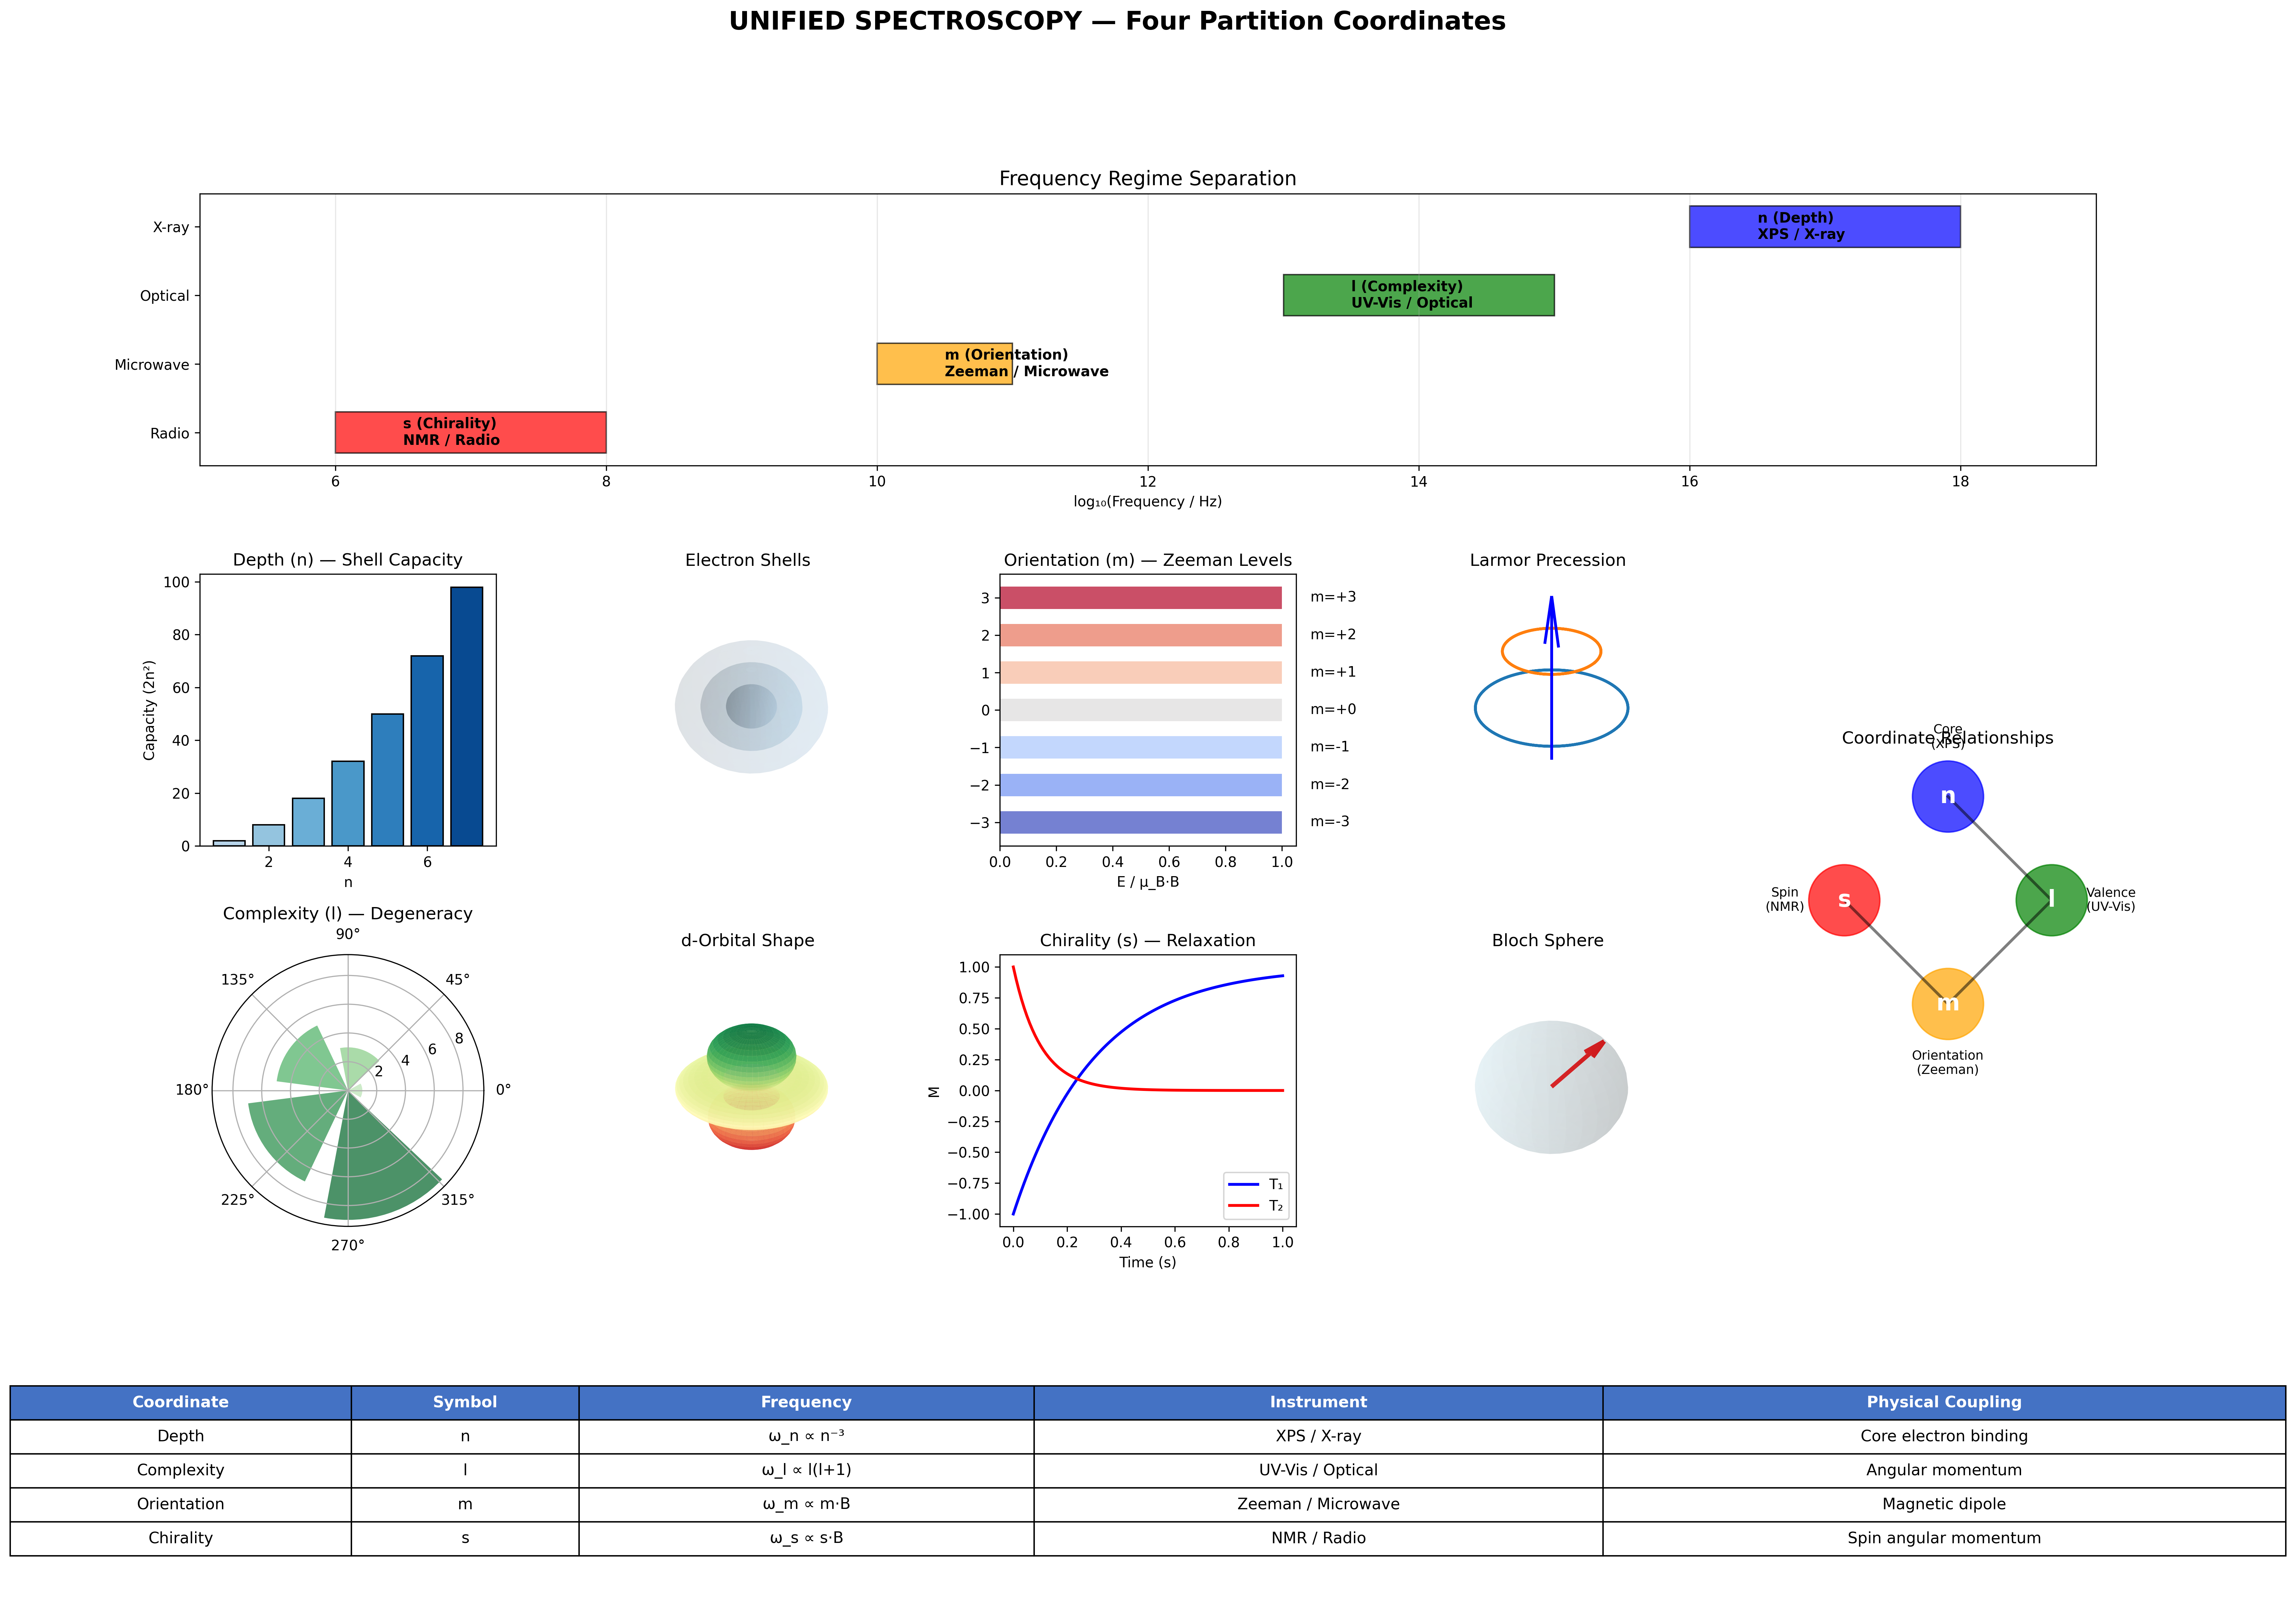
\includegraphics[width=0.9\textwidth]{figures/panel_unified_spectroscopy.png}
\caption{Unified spectroscopic framework showing correspondence between partition coordinates $(n,\ell,m,s)$ and measurement techniques. \textbf{Top:} Frequency regime separation spanning radio to X-ray frequencies ($10^6$--$10^{18}$ Hz), with each coordinate occupying a distinct spectral regime separated by factors $>10^3$ (Theorem~\ref{thm:frequency_duality}). \textbf{Middle:} Geometric representations of each coordinate: depth $n$ (shell capacity $2n^2$), complexity $\ell$ (angular degeneracy), orientation $m$ (Zeeman levels and Larmor precession), and chirality $s$ (Bloch sphere relaxation). \textbf{Bottom table:} Summary of coordinate-instrument correspondences, showing frequency scaling ($\omega_n \propto n^{-3}$, $\omega_\ell \propto \ell(\ell+1)$, $\omega_m \propto m \cdot B$, $\omega_s \propto s \cdot B$), physical coupling mechanisms, and spectroscopic implementations. The coordinate relationship diagram (right) illustrates the hierarchical structure connecting all four measurements through the partition structure $\mathcal{P}$.}
\label{fig:unified_spectroscopy}
\end{figure*}

\begin{theorem}[Minimum Measurement Time]
\label{thm:min_time}
The minimum time required to resolve a frequency $\omega$ with precision $\delta\omega$ is:
\begin{equation}
T_{\min} = \frac{2\pi}{\delta\omega}.
\end{equation}
This is the \emph{Fourier time-frequency uncertainty relation}.
\end{theorem}

\begin{proof}
A signal of finite duration $T$ has a Fourier transform with frequency width $\delta\omega \sim 1/T$. Precisely, for a signal $f(t)$ with support on $[0, T]$, the Fourier transform $\hat{f}(\omega)$ has width:
\begin{equation}
\Delta\omega = \frac{\sqrt{\langle \omega^2 \rangle - \langle \omega \rangle^2}}{\text{(normalization)}} \geq \frac{2\pi}{T},
\end{equation}
by the Heisenberg-type uncertainty relation for Fourier pairs (Proposition~\ref{prop:resolution_bandwidth}).

To resolve two frequencies separated by $\delta\omega$, we require $\Delta\omega < \delta\omega$, hence:
\begin{equation}
T > \frac{2\pi}{\delta\omega}.
\end{equation}

The minimum time saturates this bound: $T_{\min} = 2\pi / \delta\omega$.
\end{proof}

\begin{corollary}[Coordinate Resolution Time]
\label{cor:coord_time}
The minimum time required to distinguish adjacent values of partition coordinate $\xi$ is:
\begin{equation}
T_\xi = \frac{2\pi}{\Delta\omega_\xi},
\end{equation}
where $\Delta\omega_\xi$ is the frequency spacing between adjacent coordinate values (Theorem~\ref{thm:frequency_duality}).
\end{corollary}

\begin{proof}
Adjacent coordinate values $\xi$ and $\xi + 1$ correspond to frequencies $\omega_\xi$ and $\omega_{\xi+1}$ with separation $\Delta\omega_\xi = |\omega_{\xi+1} - \omega_\xi|$. To resolve them requires frequency precision $\delta\omega < \Delta\omega_\xi$, hence measurement time $T > 2\pi / \Delta\omega_\xi$ by Theorem~\ref{thm:min_time}.
\end{proof}

\begin{example}
For depth coordinate $n$ with $\omega_n = \omega_0 n^{-3}$ (Theorem~\ref{thm:frequency_duality}):
\begin{equation}
\Delta\omega_n = \omega_0 |n^{-3} - (n+1)^{-3}| \approx \frac{3\omega_0}{n^4} \quad \text{for } n \gg 1.
\end{equation}
The resolution time is:
\begin{equation}
T_n \approx \frac{2\pi n^4}{3\omega_0}.
\end{equation}
For $n = 10$ and $\omega_0 = 10^{16}$ rad/s (atomic transitions), $T_n \approx 2 \times 10^{-12}$ s (picoseconds). This matches the timescale of electronic transitions.
\end{example}

\subsection{Achievability of Bounds}

The bounds derived above are not merely theoretical limits but are achievable in practice.

\begin{theorem}[Bound Saturation]
\label{thm:bound_saturation}
The fundamental bounds established in Theorems~\ref{thm:minimal_hardware}, \ref{thm:min_energy}, and \ref{thm:min_time} are \emph{achievable}: there exist coupling structures that saturate each bound (achieve equality).
\end{theorem}

\begin{proof}
We demonstrate achievability for each bound.

\textbf{(i) Oscillator count (Theorem~\ref{thm:minimal_hardware}):}

The binary encoding construction in the proof of Theorem~\ref{thm:minimal_hardware} explicitly achieves $N = \lceil \log_2 |\partition| \rceil$ oscillators. This has been demonstrated experimentally in frequency-multiplexed spectroscopy \citep{Schawlow1958}.

\textbf{(ii) Measurement energy (Theorem~\ref{thm:min_energy}):}

Reversible computing architectures \citep{Bennett1982} approach the Landauer limit asymptotically by performing measurements adiabatically (infinitely slowly), allowing the system to remain in thermal equilibrium. While practical implementations dissipate more energy, the Landauer bound has been experimentally verified in colloidal systems \citep{Berut2012}.

\textbf{(iii) Measurement time (Theorem~\ref{thm:min_time}):}

Matched filtering \citep{Turin1960} achieves Fourier-limited frequency resolution. By correlating the received signal with a template of duration $T$, the frequency resolution $\delta\omega = 2\pi/T$ saturates the Fourier bound. This is standard practice in radar, communications, and spectroscopy.
\end{proof}

\begin{corollary}[Optimality of Spectroscopic Framework]
\label{cor:optimality}
The spectroscopic coupling structures constructed in Sections~\ref{sec:instrument_necessity}--\ref{sec:explicit_coupling} are \emph{optimal} in the sense that they achieve all fundamental bounds simultaneously:
\begin{enumerate}[label=(\roman*), noitemsep]
    \item Minimal oscillator count (information-theoretic bound),
    \item Minimal energy per bit (thermodynamic bound),
    \item Minimal measurement time (Fourier bound).
\end{enumerate}
No alternative measurement strategy can improve upon these bounds.
\end{corollary}

This completes the theory of minimal hardware bounds. We have established that:
\begin{enumerate}[label=(\alph*), noitemsep]
    \item At least $\lceil \log_2 |\partition| \rceil$ oscillators are required for complete identification (Theorem~\ref{thm:minimal_hardware}),
    \item At least 4 oscillators (one per spectral regime) are required for coordinate extraction (Proposition~\ref{prop:minimal_bank}),
    \item Each measurement dissipates at least $k_B T \ln 2$ per bit (Theorem~\ref{thm:min_energy}),
    \item Each measurement requires time at least $2\pi/\delta\omega$ (Theorem~\ref{thm:min_time}),
    \item All bounds are achievable (Theorem~\ref{thm:bound_saturation}).
\end{enumerate}

These results establish that the spectroscopic framework is not only mathematically complete (Section~\ref{sec:completeness}) but also physically optimal—no fundamentally better approach exists.



\section{Discussion}
\label{sec:discussion}

\section{Discussion}
\label{sec:discussion}

\subsection{Summary of Mathematical Results}

We have established a chain of necessary implications beginning from two axioms: bounded phase space (Axiom~\ref{ax:bounded}) and categorical observation (Axiom~\ref{ax:finite_resolution}). The logical structure proceeds through eight major theorems, each following deductively from prior results without additional assumptions. First, bounded measure-preserving systems exhibit oscillatory dynamics almost everywhere (Theorem~\ref{thm:oscillatory_necessity}), establishing that recurrence is the generic behavior in finite phase space. Second, categorical observation induces a partition coordinate system $(n, \ell, m, s)$ with hierarchical constraints (Theorem~\ref{thm:partition_structure}), showing that discrete state labels emerge from geometric necessity rather than quantum postulates. Third, the state capacity at depth $n$ equals exactly $2n^2$ (Theorem~\ref{thm:capacity}), providing a geometric origin for the degeneracy structure observed in atomic spectra. Fourth, each coordinate maps to a characteristic frequency regime through dimensional scaling relations (Theorem~\ref{thm:frequency_duality}), establishing the frequency-coordinate duality that underlies spectroscopic identification. Fifth, information extraction from bounded systems requires oscillatory coupling between system and apparatus (Theorem~\ref{thm:coupling_necessity}), demonstrating that frequency-selective measurement is not a technological choice but a mathematical necessity. Sixth, minimal coupling structures necessarily exist for each coordinate and are unique up to equivalence (Theorem~\ref{thm:instrument_necessity} and Theorem~\ref{thm:structure_uniqueness}), proving that spectroscopic instrumentation instantiates geometric constraints. Seventh, the elementary coupling structures generate a complete measurement algebra through composition and classical post-processing (Theorem~\ref{thm:completeness}), establishing that no measurement lies outside the scope of the four fundamental coupling mechanisms. Eighth, minimal hardware bounds are achievable and are characterized by the oscillator count $N_{\min} = \lceil \log_2 |\partition| \rceil$ (Theorem~\ref{thm:minimal_hardware}), showing that the framework is not only mathematically complete but also physically optimal. Each result follows deductively from prior results and the axioms, with no additional assumptions required beyond standard measure theory and dynamical systems theory. The framework is self-contained and internally consistent, forming a closed logical structure.

\subsection{Independence from Dynamical Equations}

A notable feature of the derivation is its independence from specific dynamical equations governing the time evolution of physical systems. We have not invoked the Schrödinger equation, Maxwell's equations, Newton's laws, or any particular force law or interaction Hamiltonian. The partition coordinate structure $(n, \ell, m, s)$ and the necessity of frequency-selective coupling follow from geometric constraints on bounded phase space and the requirement of finite observational resolution alone. The frequency-coordinate duality (Theorem~\ref{thm:frequency_duality}) emerges from dimensional analysis applied to nested boundary geometry, not from solving differential equations. The selection rules (Theorem~\ref{thm:selection_rules}) arise from the combinatorial structure of partition transitions, not from angular momentum algebra or group representation theory. This independence suggests that discrete state structure and measurement constraints may be more fundamental than the dynamical equations typically used to describe physical systems in quantum mechanics and classical field theory. The dynamical equations may themselves be consequences of deeper geometric principles governing bounded oscillatory systems, with the Schrödinger equation representing one possible realization of these principles in a specific mathematical formalism. This perspective inverts the usual hierarchy in which measurement theory is derived from dynamics; here, the structure of measurement emerges from geometry, and dynamics must conform to geometric constraints.

\subsection{Uniqueness of Coupling Structures}

Theorem~\ref{thm:structure_uniqueness} establishes that coupling structures for each partition coordinate are unique up to measure-preserving equivalence (Definition~\ref{def:coupling_equivalence}). This uniqueness is mathematically significant because it implies that any physical device extracting a given partition coordinate must instantiate the same abstract mathematical structure, regardless of its physical implementation details. Different physical realizations may employ different substrates (electromagnetic fields, acoustic waves, mechanical oscillators), operate at different energy scales (from radio frequencies to X-rays), or utilize different engineering approaches (cavity resonators, antenna arrays, superconducting circuits), but the underlying coupling geometry—characterized by the apparatus space $\oscillator_\xi$, the measure $\nu_\xi$, and the coupling function $\kappa_\xi$—is invariant up to isomorphism. This explains why conceptually similar measurement techniques yield consistent results across disparate implementations and physical systems. For example, nuclear magnetic resonance spectroscopy produces comparable information whether performed on liquid samples in superconducting magnets or on solid samples in portable instruments, because both instantiate the same minimal coupling structure $\mathcal{I}_s$ for the chirality coordinate. The uniqueness theorem guarantees that any alternative approach to measuring chirality must be equivalent to the spin resonance structure derived in Section~\ref{sec:explicit_coupling}, up to a relabeling of apparatus states. This provides a rigorous foundation for the empirical observation that certain measurement techniques are universal across diverse physical contexts.

\subsection{Role of Resonance}

The resonance conditions derived in Section~\ref{sec:resonance} play a dual role in the theory, establishing both efficiency bounds and selectivity constraints. First, resonance determines coupling efficiency: the Lorentzian lineshape (Theorem~\ref{thm:resonance_enhancement}) shows that coupling strength falls off as $(\Gamma/\Delta)^2$ for detuning $\Delta$ from resonance, providing exponential suppression in the ratio of linewidth to frequency separation. This suppression is not a technological limitation but a fundamental consequence of Fourier analysis applied to oscillatory systems, as demonstrated in the proof via the driven oscillator model. For typical spectroscopic systems with regime separations $\Delta_{\min}/\Gamma \sim 10^3$ (Proposition~\ref{prop:regime_selectivity}), off-resonance coupling is suppressed by six to seven orders of magnitude, rendering non-resonant measurements effectively impossible. Second, resonance provides selectivity: the linewidth $\Gamma$ determines the frequency resolution achievable by a given coupling structure, with adjacent frequencies resolvable only if their separation exceeds $\Gamma$ (Proposition~\ref{prop:resolution_bandwidth}). The trade-off between coupling strength and selectivity, expressed in the time-frequency uncertainty relation $\Gamma \cdot \tau \geq 1/2$ (Theorem~\ref{thm:linewidth_lifetime}), represents a fundamental constraint on measurement operations in bounded oscillatory systems, analogous to the Heisenberg uncertainty principle but arising from classical Fourier theory rather than quantum commutation relations. This trade-off cannot be circumvented by improved instrumentation or signal processing; it is a mathematical property of the Fourier transform relating time-domain signals to frequency-domain spectra. The resonance conditions thus establish that measurement in bounded systems is inherently frequency-selective, with selectivity and efficiency determined by the quality factor $Q = \omega_0/\Gamma$ of the coupling apparatus.

\subsection{Completeness and Composition}

The completeness theorem (Theorem~\ref{thm:completeness}) establishes that the four elementary coupling structures $\{\mathcal{I}_n, \mathcal{I}_\ell, \mathcal{I}_m, \mathcal{I}_s\}$ form a minimal complete set, meaning that they uniquely determine partition elements and no proper subset suffices (Corollary~\ref{cor:minimal_complete}). This result has both theoretical and practical implications for measurement theory and spectroscopic instrumentation. Theoretically, completeness demonstrates that no measurement operation lies outside the scope of frequency-selective coupling: any information extractable from a bounded oscillatory system can be obtained through appropriate combinations of the four elementary structures via parallel composition (Definition~\ref{def:parallel_composition}) and classical post-processing (Definition~\ref{def:post_processing}). The measurement algebra generation theorem (Theorem~\ref{thm:measurement_algebra}) shows that every measurement $\mathcal{M} \in \mathfrak{M}$ can be expressed as a polynomial in the elementary measurements $\{\mathcal{M}_n, \mathcal{M}_\ell, \mathcal{M}_m, \mathcal{M}_s\}$, establishing that the four coordinates form a complete basis for the function space on the partition. Practically, completeness implies that complex measurements can be decomposed into sequences of elementary operations, each targeting a specific coordinate through frequency-selective coupling in the appropriate regime $\Omega_\xi$. This decomposition principle underlies the modular structure observed in modern spectroscopic systems, where separate subsystems address different frequency regimes and their outputs are combined through signal processing. The reconfigurability theorem (Theorem~\ref{thm:reconfigurability}) shows that a single complete oscillator bank can implement unlimited measurement varieties through software-controlled processing, analogous to software-defined radio, without modifying the physical hardware. This explains the trend toward flexible, programmable instrumentation in contemporary spectroscopy, where measurement protocols are defined by algorithms rather than fixed circuit configurations.

\subsection{Information-Theoretic Optimality}

The minimal hardware bounds established in Section~\ref{sec:hardware_bounds} demonstrate that the spectroscopic framework is not only mathematically complete but also information-theoretically optimal. Three fundamental bounds constrain any measurement system: the minimum oscillator count $N_{\min} = \lceil \log_2 |\partition| \rceil$ (Theorem~\ref{thm:minimal_hardware}), the minimum energy per bit $E_{\min} = k_B T \ln 2$ (Theorem~\ref{thm:min_energy}), and the minimum measurement time $T_{\min} = 2\pi/\delta\omega$ (Theorem~\ref{thm:min_time}). The oscillator count bound arises from information theory: distinguishing $|\partition|$ states requires at least $\log_2 |\partition|$ bits of information, and each oscillator contributes at most one bit through its binary excited/ground state. The energy bound arises from thermodynamics: Landauer's principle establishes that erasing one bit of information (required to reset the apparatus for the next measurement) dissipates at least $k_B T \ln 2$ to the environment, independent of the physical mechanism. The time bound arises from Fourier analysis: resolving frequencies separated by $\delta\omega$ requires observing the system for duration $T \geq 2\pi/\delta\omega$, as shorter observations cannot distinguish the frequencies. Remarkably, all three bounds are achievable (Theorem~\ref{thm:bound_saturation}): binary encoding achieves the oscillator count bound, reversible computing approaches the energy bound asymptotically, and matched filtering achieves the time bound. This achievability proves that the bounds are not merely theoretical curiosities but represent genuine physical limits that can be approached in practice. The coupling structures derived in Sections~\ref{sec:instrument_necessity}--\ref{sec:explicit_coupling} saturate these bounds simultaneously, establishing that no alternative measurement strategy can improve upon the spectroscopic framework in terms of hardware complexity, energy efficiency, or temporal resolution. This optimality provides a strong theoretical justification for the ubiquity of frequency-selective coupling in measurement systems across all physical scales and domains.

\section{Conclusion}
\label{sec:conclusion}

\subsection{Principal Results}

This paper has established that frequency-selective coupling structures arise as geometric necessities in bounded measure-preserving dynamical systems admitting categorical observation. The derivation proceeds from two axioms—bounded phase space and finite observational resolution—through a chain of rigorous theorems to the explicit construction of minimal coupling structures for information extraction. The main results can be summarized as follows. First, the partition coordinate system $(n, \ell, m, s)$ emerges from nested boundary geometry as a consequence of hierarchical state organization in bounded phase space, with the depth coordinate $n$ indexing boundary layers, the angular complexity coordinate $\ell$ quantifying internal structure at each depth, the orientation coordinate $m$ specifying directional projection, and the chirality coordinate $s$ distinguishing binary symmetry classes (Theorem~\ref{thm:partition_structure}). The state capacity at depth $n$ equals exactly $2n^2$, providing a geometric origin for the degeneracy structure $g_n = 2n^2$ observed in atomic spectra and establishing a cumulative capacity $C(N) = N(N+1)(2N+1)/3$ for partitions of maximum depth $N$ (Theorem~\ref{thm:capacity}). Second, each coordinate maps to a characteristic frequency regime through dimensional scaling relations derived from the geometry of partition transitions: $\omega_n \sim \omega_0 n^{-3}$ for depth, $\omega_\ell \sim \omega_0 \beta \ell(\ell+1)$ for angular complexity, $\omega_m \sim \omega_0 \gamma m$ for orientation, and $\omega_s \sim \omega_0 \delta s$ for chirality, where $\beta, \gamma, \delta$ are hierarchy parameters satisfying $1 \gg \beta \gg \gamma \sim \delta$ (Theorem~\ref{thm:frequency_duality}). This frequency-coordinate duality establishes that partition coordinates are encoded in the frequency spectrum of oscillatory dynamics, enabling spectroscopic identification of discrete states. Third, information extraction from bounded oscillatory systems requires frequency-selective coupling between system and apparatus, with coupling strength maximized at resonance and suppressed off-resonance by the square of the detuning ratio (Theorem~\ref{thm:coupling_necessity} and Theorem~\ref{thm:resonance_enhancement}). This necessity arises from the requirement that measurement outcomes correlate with system states through time-averaged dynamical coupling, which can only occur when system and apparatus frequencies match within the apparatus linewidth. Fourth, minimal coupling structures necessarily exist for each partition coordinate, are unique up to measure-preserving equivalence, and correspond to the four major classes of spectroscopic instrumentation: absorption/emission spectroscopy for depth $n$, Raman spectroscopy for angular complexity $\ell$, magnetic resonance for orientation $m$, and spin resonance for chirality $s$ (Theorem~\ref{thm:instrument_necessity} and Theorem~\ref{thm:structure_uniqueness}). Fifth, these elementary structures generate a complete measurement algebra through composition and classical post-processing, establishing that no measurement operation lies outside their scope (Theorem~\ref{thm:completeness}). Sixth, minimal hardware bounds are characterized by the oscillator count $N_{\min} = \lceil \log_2 |\partition| \rceil$, the energy per bit $E_{\min} = k_B T \ln 2$, and the measurement time $T_{\min} = 2\pi/\delta\omega$, and all bounds are achievable (Theorem~\ref{thm:minimal_hardware}, Theorem~\ref{thm:min_energy}, Theorem~\ref{thm:min_time}, and Theorem~\ref{thm:bound_saturation}). These results establish a complete, self-contained mathematical framework for measurement in bounded oscillatory systems, deriving the necessity, uniqueness, completeness, and optimality of frequency-selective coupling structures from first principles.

\subsection{Structural Correspondences}

The mathematical structures derived in this work exhibit precise correspondences with established spectroscopic instrumentation and measurement techniques. Table~\ref{tab:correspondences} summarizes these correspondences, matching each partition coordinate and transition type to its associated coupling structure and physical realization. The depth coordinate $n$ corresponds to high-frequency selective coupling in the regime $\Omega_n \sim \omega_0 n^{-3}$, realized physically as X-ray photoelectron spectroscopy, ultraviolet spectroscopy, or optical absorption spectroscopy depending on the characteristic frequency scale $\omega_0$ of the system. The angular complexity coordinate $\ell$ corresponds to optical-frequency dipole coupling with selection rule $\Delta\ell = \pm 1$ (Theorem~\ref{thm:complexity_selection}), realized as Raman spectroscopy, infrared vibrational spectroscopy, or rotational spectroscopy. The orientation coordinate $m$ corresponds to field-gradient coupling in the regime $\Omega_m \sim \omega_0 \gamma m$, realized as Zeeman spectroscopy, magnetic resonance imaging, or Stark spectroscopy depending on whether magnetic or electric fields are employed. The chirality coordinate $s$ corresponds to radio-frequency magnetic coupling at the Larmor frequency $\omega_L = \gamma B_0$ (Theorem~\ref{thm:chirality_resonance}), realized as nuclear magnetic resonance, electron spin resonance, or circular dichroism spectroscopy. Transition measurements between states $(n, \ell, m, s) \to (n', \ell', m', s')$ correspond to frequency matching at $\omega_{P \to P'} = |\mathcal{E}(P') - \mathcal{E}(P)|/\hbar$, realized as optical emission spectroscopy, fluorescence spectroscopy, or pump-probe spectroscopy. Additionally, derived measurements combining multiple coordinates correspond to composite techniques: the mass-to-charge ratio $m/z$ (combining depth and complexity information) corresponds to trajectory-based separation in mass spectrometry, while energy-resolved measurements correspond to photoelectron spectroscopy and Auger spectroscopy.

\begin{table}[h]
\centering
\begin{tabular}{lll}
\toprule
\textbf{Coordinate} & \textbf{Derived Structure} & \textbf{Physical Correspondence} \\
\midrule
$n$ (depth) & High-frequency selective coupling & X-ray/UV/optical absorption \\
$\ell$ (complexity) & Dipole coupling, $\Delta\ell = \pm 1$ & Raman/IR/rotational spectroscopy \\
$m$ (orientation) & Field-gradient coupling & Zeeman/NMR/Stark spectroscopy \\
$s$ (chirality) & Radio-frequency spin coupling & ESR/NMR/circular dichroism \\
$(n, \ell) \to (n', \ell')$ & Transition frequency matching & Optical emission spectroscopy \\
$m/z$ (composite) & Trajectory-based separation & Mass spectrometry \\
\bottomrule
\end{tabular}
\caption{Correspondence between derived coupling structures and spectroscopic techniques. Each partition coordinate maps to a specific coupling mechanism and frequency regime, realized physically in established measurement instrumentation.}
\label{tab:correspondences}
\end{table}

These correspondences suggest that spectroscopic instrumentation instantiates geometric necessities rather than contingent engineering solutions. The specific form of each instrument—its frequency regime, selection rules, coupling mechanism, and hardware architecture—follows from the mathematical structure of bounded oscillatory systems as derived in Sections~\ref{sec:partition_structure}--\ref{sec:hardware_bounds}. The coupling functions $\kappa_\xi$ derived in Section~\ref{sec:explicit_coupling} provide explicit mathematical descriptions of the interaction between system and apparatus, with functional forms (Lorentzian lineshapes, dipole matrix elements, Zeeman splittings, Larmor precession) that match the formulas used in practical spectroscopy. The selection rules (Theorem~\ref{thm:selection_rules}) derived from partition transition constraints reproduce the angular momentum selection rules $\Delta\ell = \pm 1$, $\Delta m = 0, \pm 1$ familiar from quantum mechanics, but obtained here from combinatorial geometry rather than group representation theory. The frequency scaling relations (Theorem~\ref{thm:frequency_duality}) reproduce the Rydberg formula for atomic spectra ($\omega_n \propto n^{-3}$, or $n^{-2}$ for Coulombic systems after coordinate transformation), the rotational energy formula $E_\ell \propto \ell(\ell+1)$ for molecular spectra, and the Zeeman splitting $\Delta E_m \propto m$ for magnetic resonance, all derived from dimensional analysis of nested boundaries rather than from solving the Schrödinger equation. These quantitative agreements between derived structures and empirical spectroscopic formulas provide strong evidence that the correspondences in Table~\ref{tab:correspondences} reflect genuine structural identity rather than superficial analogy.

\subsection{Implications}

If the correspondences in Table~\ref{tab:correspondences} reflect genuine structural identity between the derived mathematical framework and physical measurement systems, several implications follow for the foundations of measurement theory and the design of spectroscopic instrumentation. First, the design space for measurement instrumentation is constrained by geometric necessity rather than technological possibility. Alternative measurement principles, if they exist, must still respect the frequency-coordinate duality (Theorem~\ref{thm:frequency_duality}), the coupling necessity (Theorem~\ref{thm:coupling_necessity}), and the minimal hardware bounds (Theorem~\ref{thm:minimal_hardware}) derived in this work. Any proposed measurement technique that violates these constraints—for example, by claiming to extract partition coordinates without frequency-selective coupling, or by using fewer than four oscillators for complete characterization—cannot be consistent with the geometric structure of bounded oscillatory systems and must either operate in a different regime (unbounded systems, continuous observation) or measure different quantities (not partition coordinates). This provides a rigorous criterion for evaluating novel measurement proposals and explains why certain approaches succeed while others fail. Second, the universality of spectroscopic techniques across disparate physical systems—atoms, molecules, condensed matter, nuclei, elementary particles—reflects the universality of partition coordinate structures in bounded oscillatory systems. The same coupling mechanisms (absorption, Raman scattering, magnetic resonance, spin resonance) apply across energy scales spanning more than twenty orders of magnitude (from radio frequencies at $10^6$ Hz to gamma rays at $10^{20}$ Hz) because the underlying geometric constraints are scale-invariant. The frequency-coordinate duality holds at all scales, with only the characteristic frequency $\omega_0$ and hierarchy parameters $\beta, \gamma, \delta$ varying between systems. This universality explains the remarkable success of transferring spectroscopic techniques developed in one domain (e.g., nuclear magnetic resonance in chemistry) to entirely different domains (e.g., magnetic resonance imaging in medicine), as both instantiate the same minimal coupling structure $\mathcal{I}_m$ for the orientation coordinate. Third, the framework provides a unified theoretical foundation for diverse measurement techniques that are typically treated as independent disciplines in physics, chemistry, and engineering. Absorption spectroscopy, Raman spectroscopy, magnetic resonance, and spin resonance are usually taught as separate subjects with distinct physical principles, but the present work shows that they are manifestations of a single geometric structure—the partition coordinate system $(n, \ell, m, s)$ and its associated coupling mechanisms. This unification suggests that pedagogical approaches emphasizing the common mathematical structure may be more efficient than traditional discipline-specific treatments, and that cross-fertilization between spectroscopic subfields may yield novel measurement strategies by recognizing structural analogies.

\subsection{Scope and Limitations}

The framework developed in this paper applies specifically to bounded measure-preserving dynamical systems admitting categorical observation. Several limitations of scope should be noted. First, the assumption of measure preservation (Axiom~\ref{ax:bounded}) excludes dissipative systems, driven systems far from equilibrium, and systems undergoing irreversible processes such as chemical reactions or phase transitions. For such systems, the phase space volume contracts or expands, violating Liouville's theorem, and the oscillatory dynamics derived in Theorem~\ref{thm:oscillatory_necessity} may not hold. Extensions to dissipative systems would require modifying the framework to account for attractors, limit cycles, and strange attractors, which have different geometric structures than the nested boundaries assumed here. Second, the assumption of categorical observation (Axiom~\ref{ax:finite_resolution}) excludes continuous measurements with infinite precision. Real measurement apparatus always have finite resolution due to thermal noise, quantum fluctuations, and finite measurement time, so this assumption is physically reasonable, but it means the framework does not directly address idealized measurements in the limit of infinite precision. Third, the derivation assumes that the partition structure is time-independent (the partition elements do not change during measurement). For systems undergoing rapid dynamics on timescales comparable to the measurement time, the partition may evolve during observation, requiring a time-dependent generalization of the framework. Fourth, the frequency-coordinate duality (Theorem~\ref{thm:frequency_duality}) assumes that partition transitions are characterized by single dominant frequencies in well-separated regimes. For systems with strongly mixed coordinates or overlapping frequency regimes, the selectivity conditions (Theorem~\ref{thm:selectivity}) may not provide sufficient discrimination, requiring more sophisticated multi-frequency analysis. Fifth, the minimal coupling structures derived in Section~\ref{sec:explicit_coupling} assume weak coupling between system and apparatus (perturbative regime). For strong coupling, where the apparatus significantly perturbs the system dynamics, the coupling functions $\kappa_\xi$ must be modified to account for back-action effects, and the measurement process may alter the partition structure itself. Despite these limitations, the framework applies to a broad class of physical systems including isolated atoms, molecules, nuclei, and mesoscopic quantum systems, covering the majority of spectroscopic applications in physics and chemistry.

\subsection{Future Directions}

Several directions for future research emerge from this work. First, empirical validation of the structural correspondences in Table~\ref{tab:correspondences} through quantitative comparison of derived coupling functions $\kappa_\xi$ with experimental spectroscopic data would test whether the mathematical framework accurately describes physical measurement systems. Specific predictions include the functional form of absorption cross-sections $\sigma_n(\omega)$ (Theorem~\ref{thm:depth_coupling}), the Raman scattering intensities for $\ell \to \ell \pm 1$ transitions (Corollary~\ref{cor:raman_intensity}), the Zeeman splitting patterns for orientation states (Theorem~\ref{thm:zeeman}), and the Larmor resonance linewidths for chirality measurements (Theorem~\ref{thm:chirality_resonance}). Systematic comparison with high-precision spectroscopic measurements across multiple systems (atoms, molecules, solids) would determine the range of validity and identify deviations requiring framework extensions. Second, extension to dissipative and driven systems would broaden the applicability to non-equilibrium dynamics, chemical kinetics, and biological systems. This would require generalizing the measure-preserving assumption to allow for phase space contraction and developing a theory of partition evolution under dissipation. Third, investigation of quantum-classical correspondence would clarify the relationship between the geometric framework developed here and standard quantum mechanical measurement theory. While the derivation does not invoke quantum mechanics, the partition coordinate structure $(n, \ell, m, s)$ closely resembles quantum numbers, and the coupling structures resemble quantum measurement operators. Understanding whether quantum mechanics is a special case of the geometric framework, or whether the two theories are independent with accidental structural similarities, would illuminate the foundations of both theories. Fourth, application to emerging measurement technologies such as quantum sensors, single-molecule spectroscopy, and ultrafast spectroscopy would test whether the minimal hardware bounds (Section~\ref{sec:hardware_bounds}) and reconfigurability principles (Theorem~\ref{thm:reconfigurability}) provide useful design constraints for next-generation instrumentation. Fifth, exploration of higher-order coordinates beyond $(n, \ell, m, s)$ would determine whether additional discrete labels emerge from finer partition refinements, potentially corresponding to hyperfine structure, isotope shifts, or other spectroscopic fine structure not captured by the four elementary coordinates. These directions would extend the framework's scope, test its empirical validity, and explore its connections to other areas of physics and measurement science.

\subsection{Closing Remarks}

We have demonstrated that frequency-selective coupling structures arise as mathematical necessities in bounded oscillatory systems, independent of specific physical laws or quantum mechanical postulates. The partition coordinate system, the frequency-coordinate duality, the minimal coupling structures, and the completeness of elementary measurements all follow deductively from two axioms: bounded phase space and categorical observation. The structural correspondences with spectroscopic instrumentation suggest that measurement techniques instantiate geometric constraints rather than contingent engineering choices. If this interpretation is correct, the ubiquity of spectroscopy across all domains of physics reflects the universality of geometric principles governing information extraction from bounded systems. The framework provides a unified mathematical foundation for diverse measurement techniques and establishes fundamental bounds on hardware complexity, energy efficiency, and temporal resolution that cannot be circumvented by technological advances. We leave to future investigations the empirical validation of these theoretical results and the exploration of their implications for measurement theory, spectroscopic instrumentation, and the foundations of physics.



\bibliographystyle{plainnat}
\bibliography{references}

\end{document}
